%%%%%%%%%%%%%%%%%%%%%%%%%%%%%%%%%%%%
% Header                           %
%%%%%%%%%%%%%%%%%%%%%%%%%%%%%%%%%%%%
% 
% Revisions: 2017-04-10 Martin R�del <martin.raedel@dlr.de>
%                       Initial draft
%               
% Contact:   Martin R�del,  martin.raedel@dlr.de
%            DLR Composite Structures and Adaptive Systems
%          
%                                 __/|__
%                                /_/_/_/  
%            www.dlr.de/fa/en      |/ DLR
% 
%%%%%%%%%%%%%%%%%%%%%%%%%%%%%%%%%%%%
% Content                          %
%%%%%%%%%%%%%%%%%%%%%%%%%%%%%%%%%%%%

\chapter{\texorpdfstring{\protect\marktool{\toolnameshort}}{\toolnameshort{}} - Quick reference guide}
\setcounter{currentlevel}{6}
\label{sec:Peridigm:QRG}

% \newpage
%%%%%%%%%%%%%%%%%%%%%%%%%%%%%%%%%%%%
% Header                           %
%%%%%%%%%%%%%%%%%%%%%%%%%%%%%%%%%%%%
%
% Revisions: 2017-04-10 Martin R�del <martin.raedel@dlr.de>
%                       Initial draft
%
% Contact:   Martin R�del,  martin.raedel@dlr.de
%            DLR Composite Structures and Adaptive Systems
%
%                                 __/|__
%                                /_/_/_/
%            www.dlr.de/fa/en      |/ DLR
%
%%%%%%%%%%%%%%%%%%%%%%%%%%%%%%%%%%%%
% Content                          %
%%%%%%%%%%%%%%%%%%%%%%%%%%%%%%%%%%%%

\leveldown{\idxPDKwDiscretization}
\label{sec:Peridigm:QRG:Discretization}
\myindex[\idxPDKeywordName]{\idxPDKwDiscretization}

%%%%%%%%%%%%%%%%%%%%%%%%%%%%%%%%%%%%
% Header                           %
%%%%%%%%%%%%%%%%%%%%%%%%%%%%%%%%%%%%
% 
% Relative sectioning with coseoul locally suppressed to be able to not have entries in the TOC
% 
% Revisions: 2017-04-10 Martin R�del <martin.raedel@dlr.de>
%                       Initial draft
%               
% Contact:   Martin R�del,  martin.raedel@dlr.de
%            DLR Composite Structures and Adaptive Systems
%          
%                                 __/|__
%                                /_/_/_/  
%            www.dlr.de/fa/en      |/ DLR
% 
%%%%%%%%%%%%%%%%%%%%%%%%%%%%%%%%%%%%
% Content                          %
%%%%%%%%%%%%%%%%%%%%%%%%%%%%%%%%%%%%

% \leveldown{Description}
% \subsection*{Description}
% \subsection*{\refstepcounter{subsection}\label{mylabel}\thesubsection\quad Description}
\subsection*{\refstepcounter{subsection}\thesubsection\quad Description}

Specify the discretization. Different types of discretization are supported, see section \ref{sec:Peridigm:Basics:InputFileFormat:Discretization}.

% \levelstay{Common information}
% \label{sec:Peridigm:QRG:Discretization:Common}

% \levelstay{Literature}
% \subsection*{Literature}
\subsection*{\refstepcounter{subsection}\thesubsection\quad Literature}

\begin{itemize}[noitemsep]
  \item \cite{SillingSA2005}
\end{itemize}

% \levelstay{Code}
% \subsection*{Code}
\subsection*{\refstepcounter{subsection}\thesubsection\quad Code}

% \leveldown{Release version}
% \subsubsection*{Release version}
% \subsection*{\refstepcounter{subsubsection}\thesubsubsection\quad Release version}
\paragraph{Release version}

Available from \href{\toolrepoversiononetwo}{version 1.2}.

% \levelstay{Required compiler options}
% \subsubsection*{Required compiler options}
% \subsection*{\refstepcounter{subsubsection}\thesubsubsection\quad Required compiler options}
\paragraph{Required compiler options}

-

% \levelstay{Routines}
% \subsubsection*{Routines}
% \subsection*{\refstepcounter{subsubsection}\thesubsubsection\quad Routines}
\paragraph{Routines}


\begin{itemize}[noitemsep]
  \item from \texttt{src/io/discretization/}:
  \begin{itemize}[noitemsep]
    \item Basically all classes
  \end{itemize}
%   \item from \texttt{src/core/}:
%   \begin{itemize}[noitemsep]
%     \item \texttt{Peridigm\_InfluenceFunction.cpp}
%     \item \texttt{Peridigm\_InfluenceFunction.hpp}
%   \end{itemize}
\end{itemize}

% \levelup{Input parameters}
% \subsection*{Input parameters}
\subsection*{\refstepcounter{subsection}\label{sec:Peridigm:QRG:Discretization:Common:Parameters}\thesubsection\quad Input parameters}
% \label{sec:Peridigm:QRG:Discretization:Common:Parameters}

% \leveldown{List}
% \subsubsection*{List}
% \subsection*{\refstepcounter{subsubsection}\thesubsubsection\quad List}
\paragraph{List}

\begin{tabularx}{\linewidth}{lcccX}
\toprule
Name            & Type          & Required      & Default       & Description           \\
\midrule
Type\textsuperscript{\ref{enm:Peridigm:QRG:Discretization:Remark:Type}}            & string        & \checkmark    & -             & Mesh key: 
``\idxPDKwExodus''\myindex[\idxPDKeywordName]{\idxPDKwExodus} | 
``\idxPDKwTextFile''\myindex[\idxPDKeywordName]{\idxPDKwTextFile} | 
``\idxPDKwAlbany''\myindex[\idxPDKeywordName]{\idxPDKwAlbany} | 
``\idxPDKwPdQuickGrid''\myindex[\idxPDKeywordName]{\idxPDKwPdQuickGrid}       \\
\idxPDKwInputMeshFile\myindex[\idxPDKeywordName]{\idxPDKwInputMeshFile} & string        & \checkmark    & -             & Name of the mesh file in the same folder\\
\idxPDKwInfluenceFunction\myindex[\idxPDKeywordName]{\idxPDKwInfluenceFunction}\textsuperscript{\ref{enm:Peridigm:QRG:Discretization:Remark:InfluenceFunction}} & string     & -             & ``\idxPDKwOne''       &
``\idxPDKwOne''\myindex[\idxPDKeywordName]{\idxPDKwOne} | 
``\idxPDKwParabolicDecay''\myindex[\idxPDKeywordName]{\idxPDKwParabolicDecay} | 
``\idxPDKwGaussian''\myindex[\idxPDKeywordName]{\idxPDKwGaussian} | 
User defined\\
Omit Bonds Between Blocks\textsuperscript{\ref{enm:Peridigm:QRG:Discretization:Remark:OmitBondsBetweenBlocks}}   & string        & -     & -     & ``All'' | ``None'' | List of blocks to ignore bonds between        \\
\idxPDKwBondFilters\textsuperscript{\ref{enm:Peridigm:QRG:Discretization:Remark:BondFilters}}  & List & -     & -     & List of \idxPDKwBondFilters\\
\bottomrule
\end{tabularx}

% \levelstay{Remarks}
% \subsubsection*{Remarks}
% \subsection*{\refstepcounter{subsubsection}\thesubsubsection\quad Remarks}
\paragraph{Remarks}

\begin{enumerate}[noitemsep]
  \item \label{enm:Peridigm:QRG:Discretization:Remark:Type} Discretization type:
    \begin{description}[noitemsep,labelindent=0pt,style=multiline,leftmargin=0.2\linewidth]
      \item[Text File:] ASCII text file mesh input, see \ref{sec:Peridigm:Basics:InputFileFormat:Discretization:Textfile}
      \item[Exodus:] Binary Exodus mesh input, see \ref{sec:Peridigm:Basics:InputFileFormat:Discretization:Exodus}
      \item[Albany:] Mesh from Albany multiphyisics code, see \ref{sec:Peridigm:Basics:InputFileFormat:Discretization:Albany}
      \item[PdQuickGrid:] Mesh creation inside \marktool{\toolname} for simple cubical geometries, see \ref{sec:Peridigm:Basics:InputFileFormat:Discretization:PdQuickGrid}
    \end{description}
  \item \label{enm:Peridigm:QRG:Discretization:Remark:InfluenceFunction} See section \ref{sec:Peridigm:QRG:Discretization:Tools:InfluenceFunction}
  \item \label{enm:Peridigm:QRG:Discretization:Remark:OmitBondsBetweenBlocks} Possible values for keyword \textit{Omit Bonds Between Blocks}:
    \begin{itemize}[noitemsep]
      \item ``All''
      \item ``None''
      \item Discrete definition of individual block pairs seems to be not possible at the moment (see \texttt{src/io/discretization/Peridigm\_ExodusDiscretization.cpp} lines 744-762)
    \end{itemize}
  \item\label{enm:Peridigm:QRG:Discretization:Remark:BondFilters} Additional lines might be added by the use of the discretization tools described in section \ref{sec:Peridigm:QRG:DiscretizationTools}.
\end{enumerate}

% \levelup{Exemplary input section}
% \subsection*{Exemplary input section}
\subsection*{\refstepcounter{subsection}\thesubsection\quad Exemplary input section}

% \leveldown{\protect\nameref{sec:Peridigm:Basics:InputFileFormat:Discretization:Textfile}}
% \subsubsection*{\protect\nameref{sec:Peridigm:Basics:InputFileFormat:Discretization:Textfile}}
% \subsection*{\refstepcounter{subsubsection}\thesubsubsection\quad \protect\nameref{sec:Peridigm:Basics:InputFileFormat:Discretization:Textfile}}
\paragraph{\nameref{sec:Peridigm:Basics:InputFileFormat:Discretization:Textfile}}

% \leveldown{XML format}
\subparagraph*{XML format}

\begingroup
\lstset{breaklines=true}
\begin{code}
<ParameterList name="Discretization">
  <Parameter name="Type" type="string" value="Text File" />
  <Parameter name="Input Mesh File" type="string" value="Compression_QS_3x2x2_TextFile.txt"/>
</ParameterList>
\end{code}
\endgroup

% \levelstay{Free format}
\subparagraph*{Free format}

-

% \levelstay{YAML format}
\subparagraph*{YAML format}

-

% \levelup{\nameref{sec:Peridigm:Basics:InputFileFormat:Discretization:Exodus}}
% \subsubsection*{\protect\nameref{sec:Peridigm:Basics:InputFileFormat:Discretization:Exodus}}
% \subsection*{\refstepcounter{subsubsection}\thesubsubsection\quad \protect\nameref{sec:Peridigm:Basics:InputFileFormat:Discretization:Exodus}}
\paragraph{\nameref{sec:Peridigm:Basics:InputFileFormat:Discretization:Exodus}}

% \leveldown{XML format}
\subparagraph*{XML format}

\begingroup
\lstset{breaklines=true}
\begin{code}
<ParameterList name="Discretization">
  <Parameter name="Type" type="string" value="Exodus" />
  <Parameter name="Input Mesh File" type="string" value="Bar.g"/>
  <Parameter name="Omit Bonds Between Blocks" type="string" value="All" />
</ParameterList>
\end{code}
\endgroup

% \levelstay{Free format}
\subparagraph*{Free format}

\begingroup
\lstset{breaklines=true}
\begin{code}
Discretization
  Type "Exodus"
  Input Mesh File "mesh.g"
  Influence Function "One"
\end{code}
\endgroup

% \levelstay{YAML format}
\subparagraph*{YAML format}

-

% \levelup{\nameref{sec:Peridigm:Basics:InputFileFormat:Discretization:Albany}}
% \subsubsection*{\protect\nameref{sec:Peridigm:Basics:InputFileFormat:Discretization:Albany}}
% \subsection*{\refstepcounter{subsubsection}\thesubsubsection\quad \protect\nameref{sec:Peridigm:Basics:InputFileFormat:Discretization:Albany}}
\paragraph{\nameref{sec:Peridigm:Basics:InputFileFormat:Discretization:Albany}}

% \leveldown{XML format}
\subparagraph*{XML format}

-

% \levelstay{Free format}
\subparagraph*{Free format}

-

% \levelstay{YAML format}
\subparagraph*{YAML format}

-

% \levelup{\nameref{sec:Peridigm:Basics:InputFileFormat:Discretization:PdQuickGrid}}
% \subsubsection*{\protect\nameref{sec:Peridigm:Basics:InputFileFormat:Discretization:PdQuickGrid}}
% \subsection*{\refstepcounter{subsubsection}\thesubsubsection\quad \protect\nameref{sec:Peridigm:Basics:InputFileFormat:Discretization:PdQuickGrid}}
\paragraph{\nameref{sec:Peridigm:Basics:InputFileFormat:Discretization:PdQuickGrid}}

% \leveldown{XML format}
\subparagraph*{XML format}

-

% \levelstay{Free format}
\subparagraph*{Free format}

-

% \levelstay{YAML format}
\subparagraph*{YAML format}

-

% \levelmultiup{List of examples}{2}
% \subsection*{List of examples}
\subsection*{\refstepcounter{subsection}\thesubsection\quad List of examples}

% \leveldown{\nameref{sec:Peridigm:Basics:InputFileFormat:Discretization:Textfile}}
% \subsubsection*{\protect\nameref{sec:Peridigm:Basics:InputFileFormat:Discretization:Textfile}}
% \subsubsection*{\refstepcounter{subsubsection}\thesubsubsection\quad \protect\nameref{sec:Peridigm:Basics:InputFileFormat:Discretization:Textfile}}
\paragraph{\nameref{sec:Peridigm:Basics:InputFileFormat:Discretization:Textfile}}

\begin{itemize}[noitemsep]
%   \item From \texttt{examples/}:
%   \begin{itemize}[noitemsep]
%     \item \texttt{examples/tensile\_test/tensile\_test.peridigm}
%   \end{itemize}
  \item From \texttt{test/regression/}:
  \begin{itemize}[noitemsep]
    \item \texttt{Compression\_QS\_3x2x2\_TextFile/Compression\_QS\_3x2x2\_TextFile.xml}
  \end{itemize}
  \item From \texttt{test/verification/}:
  \begin{itemize}[noitemsep]
    \item \texttt{MultipleHorizons/MultipleHorizons.xml}
  \end{itemize}
\end{itemize}

% \levelstay{\nameref{sec:Peridigm:Basics:InputFileFormat:Discretization:Exodus}}
% \subsubsection*{\protect\nameref{sec:Peridigm:Basics:InputFileFormat:Discretization:Exodus}}
% \subsubsection*{\refstepcounter{subsubsection}\thesubsubsection\quad \protect\nameref{sec:Peridigm:Basics:InputFileFormat:Discretization:Exodus}}
\paragraph{\nameref{sec:Peridigm:Basics:InputFileFormat:Discretization:Exodus}}

\begin{itemize}[noitemsep]
  \item For input parameter \textit{Influence Function}:
    \begin{itemize}[noitemsep]
    \item \verb+/test/verification/Compression_3x1x1_InfluenceFunction/Compression_3x1x1_InfluenceFunction.xml+
    \end{itemize}
  \item For input parameter \textit{Omit Bonds Between Blocks}:
    \begin{itemize}[noitemsep]
    \item \verb+/test/regression/Bar_TwoDisconnectedPieces_QS/Bar.xml+
    \end{itemize}
\end{itemize}

% \levelstay{\nameref{sec:Peridigm:Basics:InputFileFormat:Discretization:Albany}}
% \subsubsection*{\protect\nameref{sec:Peridigm:Basics:InputFileFormat:Discretization:Albany}}
% \subsubsection*{\refstepcounter{subsubsection}\thesubsubsection\quad \protect\nameref{sec:Peridigm:Basics:InputFileFormat:Discretization:Albany}}
\paragraph{\nameref{sec:Peridigm:Basics:InputFileFormat:Discretization:Albany}}

% \levelstay{\nameref{sec:Peridigm:Basics:InputFileFormat:Discretization:PdQuickGrid}}
% \subsubsection*{\protect\nameref{sec:Peridigm:Basics:InputFileFormat:Discretization:PdQuickGrid}}
% \subsubsection*{\refstepcounter{subsubsection}\thesubsubsection\quad \protect\nameref{sec:Peridigm:Basics:InputFileFormat:Discretization:PdQuickGrid}}
\paragraph{\nameref{sec:Peridigm:Basics:InputFileFormat:Discretization:PdQuickGrid}}

% Set the counter to get the following things right
\setcounter{currentlevel}{3}


\newpage
%%%%%%%%%%%%%%%%%%%%%%%%%%%%%%%%%%%%
% Header                           %
%%%%%%%%%%%%%%%%%%%%%%%%%%%%%%%%%%%%
%
% Revisions: 2017-04-10 Martin R�del <martin.raedel@dlr.de>
%                       Initial draft
%
% Contact:   Martin R�del,  martin.raedel@dlr.de
%            DLR Composite Structures and Adaptive Systems
%
%                                 __/|__
%                                /_/_/_/
%            www.dlr.de/fa/en      |/ DLR
%
%%%%%%%%%%%%%%%%%%%%%%%%%%%%%%%%%%%%
% Content                          %
%%%%%%%%%%%%%%%%%%%%%%%%%%%%%%%%%%%%

\levelmultiup{Discretization tools}{2}
\label{sec:Peridigm:QRG:DiscretizationTools}

\leveldown{Preliminaries}

Tools to modify the discretization behavior.

% \newpage
%%%%%%%%%%%%%%%%%%%%%%%%%%%%%%%%%%%%
% Header                           %
%%%%%%%%%%%%%%%%%%%%%%%%%%%%%%%%%%%%
% 
% Revisions: 2017-04-10 Martin R�del <martin.raedel@dlr.de>
%                       Initial draft
%               
% Contact:   Martin R�del,  martin.raedel@dlr.de
%            DLR Composite Structures and Adaptive Systems
%          
%                                 __/|__
%                                /_/_/_/  
%            www.dlr.de/fa/en      |/ DLR
% 
%%%%%%%%%%%%%%%%%%%%%%%%%%%%%%%%%%%%
% Content                          %
%%%%%%%%%%%%%%%%%%%%%%%%%%%%%%%%%%%%

\levelstay{\idxPDKwBondFilters}
\label{sec:Peridigm:QRG:Discretization:Tools:BondFilters}
\myindex[\idxPDKeywordName]{\idxPDKwBondFilters}

\leveldown{Description}

A method to omit bonds in the discretization.

\levelstay{Code}

Dependent on the type of discretization the following classes are used:

\begin{itemize}[noitemsep]
  \item from \texttt{src/io/discretization/}:
  \begin{itemize}[noitemsep]
    \item \texttt{Peridigm\_AlbanyDiscretization.cpp}
    \item \texttt{Peridigm\_AlbanyDiscretization.hpp}
    \item \texttt{Peridigm\_ExodusDiscretization.cpp}
    \item \texttt{Peridigm\_ExodusDiscretization.hpp}
    \item \texttt{Peridigm\_PdQuickGridDiscretization.hpp}
    \item \texttt{Peridigm\_PdQuickGridDiscretization.cpp}
    \item \texttt{Peridigm\_TextFileDiscretization.hpp}
    \item \texttt{Peridigm\_TextFileDiscretization.cpp}
  \end{itemize}
\end{itemize}

All extend the super-class

\begin{itemize}[noitemsep]
  \item \verb+/src/io/discretization/Peridigm_Discretization.cpp+
  \item \verb+/src/io/discretization/Peridigm_Discretization.hpp+
\end{itemize}

Each class uses the method from the super-class :

\verb+PeridigmNS::Discretization::createBondFilters+

\levelstay{Input parameters}

\leveldown{List}

\begin{tabularx}{\linewidth}{lcccX}
\toprule
Name                    & Type   & Required   & Default & Description           \\
\midrule
Type                    & string & \checkmark & - & ``\idxPDKwRectangularPlane'' \\
Normal\_X               & double & \checkmark & - & $\glssymbol{symb:scalar:coord:global:x}$-component of the cutting plane normal vector\\
Normal\_Y               & double & \checkmark & - & $\glssymbol{symb:scalar:coord:global:y}$-component of the cutting plane normal vector\\
Normal\_Z               & double & \checkmark & - & $\glssymbol{symb:scalar:coord:global:z}$-component of the cutting plane normal vector\\
Lower\_Left\_Corner\_X  & double & \checkmark & - & $\glssymbol{symb:scalar:coord:global:x}$ component of lower left rectangle corner\\
Lower\_Left\_Corner\_Y  & double & \checkmark & - & $\glssymbol{symb:scalar:coord:global:y}$ component of lower left rectangle corner\\
Lower\_Left\_Corner\_Z  & double & \checkmark & - & $\glssymbol{symb:scalar:coord:global:z}$ component of lower left rectangle corner\\
Bottom\_Unit\_Vector\_X & double & \checkmark & - & $\glssymbol{symb:scalar:coord:global:x}$ component of rectangle bottom edge direction vector\\
Bottom\_Unit\_Vector\_Y & double & \checkmark & - & $\glssymbol{symb:scalar:coord:global:y}$ component of rectangle bottom edge direction vector\\
Bottom\_Unit\_Vector\_Z & double & \checkmark & - & $\glssymbol{symb:scalar:coord:global:z}$ component of rectangle bottom edge direction vector\\
Bottom\_Length          & double & \checkmark & - & Length of rectangle bottom and top edges\\
Side\_Length            & double & \checkmark & - & Length of rectangle left and right edges\\
\bottomrule
\end{tabularx}

\levelstay{Remarks}

\begin{enumerate}[noitemsep]
  \item \idxPDKwBondFilters{} cause the bonds to not be created in the first place
  \item For type ``\idxPDKwRectangularPlane'':
  \begin{itemize}[noitemsep]
    \item Define a rectangular cut plane where all bonds are released prior to the simulation.
  \end{itemize}
  \item It is suggested to define the output variable Number\_Of\_Neighbors in order to confirm that the bond filter is in the right place. It always seems to take me multiple tries to get it right.
\end{enumerate}

\levelstay{Usage}

The input parameters form a 2D rectangle in 3D space. Bonds that would pass through the rectangle are not formed, which creates a pre-crack.

\begin{figure}[htbp]
  \centering
  %%%%%%%%%%%%%%%%%%%%%%%%%%%%%%%%%%%%
% Header                           %
%%%%%%%%%%%%%%%%%%%%%%%%%%%%%%%%%%%%
% 
% This file handles all things considering the pgfplots package
% 
% Revisions: 2017-04-10 Martin Raedel <martin.raedel@dlr.de>
%                       Initial draft
%               
% Contact:   Martin Raedel,  martin.raedel@dlr.de
%            DLR Composite Structures and Adaptive Systems
%          
%                                 __/|__
%                                /_/_/_/  
%            www.dlr.de/fa/en      |/ DLR
% 
%%%%%%%%%%%%%%%%%%%%%%%%%%%%%%%%%%%%
% Content                          %
%%%%%%%%%%%%%%%%%%%%%%%%%%%%%%%%%%%%

\begin{tikzpicture}
  % External figure
  \node[anchor=south west,inner sep=0] (image) at (0,0) {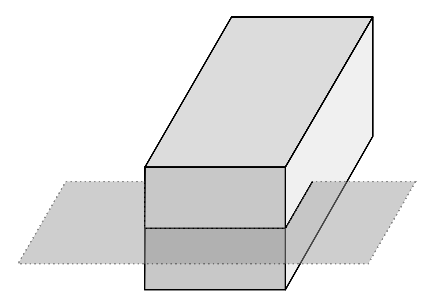
\includegraphics[width=0.7\linewidth]{Figures/Peridigm/Discretization_BondFilters_RectangularPlane}};
% Figure scope
  \begin{scope}[
    x={(image.south east)},
    y={(image.north west)},
  ]
    % Coordinates
    \coordinate (p1)  at (0.005,0.100);
    \coordinate (p2)  at (0.878,0.100);
    \coordinate (p3)  at (0.995,0.397);
    \coordinate (p4)  at (0.125,0.397);
    \coordinate (pn)  at (0.250,0.300);
    
    \coordinate (p1v) at ($(p1)-(0.0,9ex)$);
    \coordinate (p2v) at ($(p2)-(0.0,9ex)$);
    \coordinate (p2s) at ($(p2)+(1em,0.0)$);
    \coordinate (p3s) at ($(p3)+(1em,0.0)$);
    % Dots
    \draw[black,fill=black] (p1) circle (2pt);
    \draw[black]            (p2) circle (2pt);
    \draw[black]            (p3) circle (2pt);
    \draw[black]            (p4) circle (2pt);
    % Nodes
    \node[anchor=east,align=center]  at (p1) {Lower\_\\Left\_\\Corner}; 
    \node[anchor=north,xshift=0.5em] at (p1) {1}; 
    \node[anchor=north]              at (p2) {2};
    \node[anchor=south]              at (p3) {3};
    \node[anchor=south]              at (p4) {4};
    % Arrows
    \draw[-latex,very thick] (p1) -- ($(p1)+(5em,0.0)$) node [below,align=center] {Bottom\_\\Unit\_\\Vector};
    \draw[-latex,very thick] (pn) -- ($(pn)+(0.0,5em)$) node [above] {Normal};
    \draw[latex-latex,very thick] (p1v) -- (p2v) node [midway, anchor=north, align=center] {Bottom\_Length};
    \draw[latex-latex,very thick] (p2s) -- (p3s) node [midway, anchor=west, align=center,xshift=0.5em] {Side\_\\Length};
    % Labels
    \node[anchor=north east]         (modellabel) at (0.4,0.90) {Model};
    \node[anchor=north,align=center] (planelabel) at (0.8,0.03) {Rectangular\\Plane};
    \draw (modellabel) -- (0.55,0.8);
    \draw (planelabel) -- (0.82,0.2);
    % Help grid and labels
    %\pic{myimagegrid};
  \end{scope}
\end{tikzpicture}

  \caption{Bond Filter - Rectangular Plane}
  \label{fig:Peridigm:QRG:Discretization:Tools:BondFilter:RectangularPlane}
\end{figure}

\begin{tabularx}{\linewidth}{lX}
\textit{Lower\_Left\_Corner}  & Point in 3D which defines the origin of the rectangle in its lower left corner, here named ``1''.  \\
\textit{Bottom\_Unit\_Vector} & Vector of unit length in 3D defining the direction along the bottom of the rectangle, here from ``1'' to ``2''.  \\
\textit{Normal}               & Vector in 3D that defines the normal direction of the rectangle. From this and \textit{Bottom\_Unit\_Vector} the vector of the other side of the rectangle, here from ``1'' to ``4'', is calculated internally using the vector or cross product.  \\
\textit{Bottom\_Length}       & Length of the side along \textit{Bottom\_Unit\_Vector}, so the length between ``1'' to ``2'' and ``3'' to ``4''.  \\
\textit{Side\_Length}         & Length of the others two sides, here ``1'' to ``4'' and ``2'' to ``3''.
\end{tabularx}

\levelup{Exemplary input section}

\leveldown{XML-format}

from \verb+/test/regression/PrecrackedPlate/PrecrackedPlate.xml+:

\begingroup
\lstset{breaklines=true}
\begin{code}
<ParameterList name="Discretization">
  <Parameter name="Type" type="string" value="Exodus" />
  <Parameter name="Input Mesh File" type="string" value="Plate.g"/>
  <ParameterList name="Bond Filters">
    <ParameterList name="My First Bond Filter">
      <Parameter name="Type" type="string" value="Rectangular_Plane"/>
      <Parameter name="Normal_X" type="double" value="0.0"/>
      <Parameter name="Normal_Y" type="double" value="1.0"/>
      <Parameter name="Normal_Z" type="double" value="0.0"/>
      <Parameter name="Lower_Left_Corner_X" type="double" value="-10.0"/>
      <Parameter name="Lower_Left_Corner_Y" type="double" value="0.0"/>
      <Parameter name="Lower_Left_Corner_Z" type="double" value="-10.0"/>
      <Parameter name="Bottom_Unit_Vector_X" type="double" value="1.0"/>
      <Parameter name="Bottom_Unit_Vector_Y" type="double" value="0.0"/>
      <Parameter name="Bottom_Unit_Vector_Z" type="double" value="0.0"/>
      <Parameter name="Bottom_Length" type="double" value="10"/>
      <Parameter name="Side_Length" type="double" value="20"/>
    </ParameterList>
  </ParameterList>
</ParameterList>
\end{code}
\endgroup

\levelstay{Free format}

\begingroup
\lstset{breaklines=true}
\begin{code}
Discretization
  ...
  Bond Filters
    bond_filter-1
      Type "Rectangular_Plane"
      Normal_X 0.0
      Normal_Y -1.0
      Normal_Z 0.0
      Lower_Left_Corner_X -0.1
      Lower_Left_Corner_Y 0.0
      Lower_Left_Corner_Z -0.1
      Bottom_Unit_Vector_X 0.0
      Bottom_Unit_Vector_Y 0.0
      Bottom_Unit_Vector_Z 1.0
      Bottom_Length 0.2
      Side_Length 10.1
\end{code}
\endgroup

\levelstay{YAML format}

-

\levelup{List of examples}

\begin{itemize}[noitemsep]
%   \item From \texttt{examples/}:
%   \begin{itemize}[noitemsep]
%     \item \texttt{examples/tensile_test/tensile_test.peridigm}
%   \end{itemize}
  \item From \texttt{test/regression/}:
  \begin{itemize}[noitemsep]
    \item \texttt{PrecrackedPlate/PrecrackedPlate.xml}
    \item \texttt{PrecrackedPlateTwoCracks/PrecrackedPlateTwoCracks.xml}
  \end{itemize}
%   \item From \texttt{test/verification/}:
%   \begin{itemize}[noitemsep]
%     \item \texttt{Contact_Friction/Contact_Friction.xml}
%   \end{itemize}
\end{itemize}
% \begin{itemize}[noitemsep]
%   \item \texttt{/test/regression/PrecrackedPlate/PrecrackedPlate.xml}
%   \item \texttt{/test/regression/PrecrackedPlateTwoCracks/PrecrackedPlateTwoCracks.xml}
% \end{itemize}
 

\newpage
%%%%%%%%%%%%%%%%%%%%%%%%%%%%%%%%%%%%
% Header                           %
%%%%%%%%%%%%%%%%%%%%%%%%%%%%%%%%%%%%
%
% Revisions: 2017-04-10 Martin R�del <martin.raedel@dlr.de>
%                       Initial draft
%
% Contact:   Martin R�del,  martin.raedel@dlr.de
%            DLR Composite Structures and Adaptive Systems
%
%                                 __/|__
%                                /_/_/_/
%            www.dlr.de/fa/en      |/ DLR
%
%%%%%%%%%%%%%%%%%%%%%%%%%%%%%%%%%%%%
% Content                          %
%%%%%%%%%%%%%%%%%%%%%%%%%%%%%%%%%%%%

\levelup{\idxPDKwInfluenceFunction}
\label{sec:Peridigm:QRG:Discretization:Tools:InfluenceFunction}
\myindex[\idxPDKeywordName]{\idxPDKwInfluenceFunction}

\leveldown{Description}

The influence function in the peridynamic theory is used to weight the contribution of all the bonds participating in the computation of volume-dependent properties dependent of the distance to the family origin.

\levelstay{Literature}

\begin{itemize}[noitemsep]
  \item \cite{SelesonP2011}
  \item \cite{TupekMR2013}
\end{itemize}

\levelstay{Code}

\leveldown{Release version}

Available from \href{\toolrepoversiononetwo}{version 1.2}.

\levelstay{Required compiler options}

-

\levelstay{Routines}

\begin{itemize}[noitemsep]
  \item from \texttt{src/core/}:
  \begin{itemize}[noitemsep]
    \item \texttt{Peridigm\_Peridigm\_InfluenceFunction.cpp}
    \item \texttt{Peridigm\_Peridigm\_InfluenceFunction.hpp}
  \end{itemize}
\end{itemize}

% Each class uses the method as:
% \begin{itemize}[noitemsep]
% \item \verb+PeridigmNS::InfluenceFunction::functionPointer m_OMEGA;+
% 
% The function value can be obtained by
% \item \verb+omega = m_OMEGA(initialDistance, m_horizon);+
% \end{itemize}

\levelup{Input parameters}

\leveldown{List}

The influence function is not an individual object. Therefore, no parameter list is required here.

\levelstay{Remarks}

\begin{enumerate}[noitemsep]
  \item The influence function is defined for the whole model.
  \item Function values are dependent of the bond length $\lVert\glssymbol{symb:vector:pd:bond:undeformed}\rVert$ and the local horizon $\glssymbol{symb:scalar:pd:horizon}$
  \item The influence functions in \autoref{fig:Peridigm:QRG:Discretization:Common:InfluenceFunctions} are pre-implemented. Each unrecognized string is assumed to be an user-defined influence function. The default value is set to \textit{\idxPDKwOne} in case the keyword is not specified, see \texttt{Peridigm.cpp}.
    
  \begin{figure}[htbp]
    \def\figxlabel{$\frac{\lVert\glssymbol{symb:vector:pd:bond:undeformed}\rvert|}{\glssymbol{symb:scalar:pd:horizon}}$}
    \def\figylabel{$\glssymbol{symb:scalar:pd:function:influence:radial}\left(\glssymbol{symb:vector:pd:bond:undeformed}\right)$}
    %\def\figwidth{\linewidth}
    \setlength{\figwidth}{0.33\linewidth}
    \setlength{\figheight}{\figwidth}
    
    \begin{subfigure}{\figwidth}
      \centering
      \tikzexternalenable
      \tikzsetnextfilename{Discretization_InfluenceFunction_One}
      %%%%%%%%%%%%%%%%%%%%%%%%%%%%%%%%%%%%
% Header                           %
%%%%%%%%%%%%%%%%%%%%%%%%%%%%%%%%%%%%
% 
% Revisions: 2017-04-10 Martin R�del <martin.raedel@dlr.de>
%                       Initial draft
%               
% Contact:   Martin R�del,  martin.raedel@dlr.de
%            DLR Composite Structures and Adaptive Systems
%          
%                                 __/|__
%                                /_/_/_/  
%            www.dlr.de/fa/en      |/ DLR
% 
%%%%%%%%%%%%%%%%%%%%%%%%%%%%%%%%%%%%
% Content                          %
%%%%%%%%%%%%%%%%%%%%%%%%%%%%%%%%%%%%

\begin{tikzpicture}
  \begin{axis}[influencefunctionaxis style]
    \addplot[\plotcolor]{1.0};
  \end{axis}
\end{tikzpicture}
      \tikzexternaldisable
      \caption{\idxPDKwOne}
      \label{fig:Peridigm:QRG:Discretization:Common:InfluenceFunction:One}
    \end{subfigure}%
    \hfill
    \begin{subfigure}{\figwidth}
      \centering
      \tikzexternalenable
      \tikzsetnextfilename{Discretization_InfluenceFunction_ParabolicDecay}
      %%%%%%%%%%%%%%%%%%%%%%%%%%%%%%%%%%%%
% Header                           %
%%%%%%%%%%%%%%%%%%%%%%%%%%%%%%%%%%%%
% 
% Revisions: 2017-04-10 Martin R�del <martin.raedel@dlr.de>
%                       Initial draft
%               
% Contact:   Martin R�del,  martin.raedel@dlr.de
%            DLR Composite Structures and Adaptive Systems
%          
%                                 __/|__
%                                /_/_/_/  
%            www.dlr.de/fa/en      |/ DLR
% 
%%%%%%%%%%%%%%%%%%%%%%%%%%%%%%%%%%%%
% Content                          %
%%%%%%%%%%%%%%%%%%%%%%%%%%%%%%%%%%%%

\begin{tikzpicture}[
  declare function={
    parabolicdecay(\x) = (\x<=0.5) * (1.0)   +
                          (\x> 0.5) * (-4.0*\x*\x+4.0*\x);
  }
]
  \begin{axis}[influencefunctionaxis style]
    \addplot[\plotcolor]{parabolicdecay(x)};
  \end{axis}
\end{tikzpicture}
      \tikzexternaldisable
      \caption{\idxPDKwParabolicDecay}
      \label{fig:Peridigm:QRG:Discretization:Common:InfluenceFunction:ParabolicDecay}
    \end{subfigure}%
    \hfill
    \begin{subfigure}{\figwidth}
  %       \def\legendentrywithciteexpansion{\cite{SelesonP2014b}}
      \centering
  %       \tikzexternalenable
  %       \tikzsetnextfilename{Discretization_InfluenceFunction_Gaussian}
      %%%%%%%%%%%%%%%%%%%%%%%%%%%%%%%%%%%%
% Header                           %
%%%%%%%%%%%%%%%%%%%%%%%%%%%%%%%%%%%%
% 
% Revisions: 2017-04-10 Martin R�del <martin.raedel@dlr.de>
%                       Initial draft
%               
% Contact:   Martin R�del,  martin.raedel@dlr.de
%            DLR Composite Structures and Adaptive Systems
%          
%                                 __/|__
%                                /_/_/_/  
%            www.dlr.de/fa/en      |/ DLR
% 
%%%%%%%%%%%%%%%%%%%%%%%%%%%%%%%%%%%%
% Content                          %
%%%%%%%%%%%%%%%%%%%%%%%%%%%%%%%%%%%%

\begin{tikzpicture}
  \begin{axis}[
    influencefunctionaxis style,
    legend pos=south west,
  ]
    \addplot[\plotcolor]{e^(-x*x/(0.4*0.4))};
    \addlegendentry{\cite{SelesonP2014b}}
    \addplot[black,dashed]{e^(-x*x)};
    \addlegendentry{\cite{TupekMR2013}}
  \end{axis}
\end{tikzpicture}
  %       \tikzexternaldisable
      \caption{\idxPDKwGaussian}
      \label{fig:Peridigm:QRG:Discretization:Common:InfluenceFunction:Gaussian}
    \end{subfigure}%
    \caption{Influence functions}
    \label{fig:Peridigm:QRG:Discretization:Common:InfluenceFunctions}
  \end{figure}
  \item For further information on the effect of the influence function see: \cite{SelesonP2011} \& \cite{LittlewoodD2015}.
  \item Other Influence functions and their usage can be found in \cite{SelesonP2014b}.  The ``\idxPDKwParabolicDecay'' is used in \cite{LittlewoodD2013b}. Several different functions can be found in the literature for the ``\idxPDKwGaussian'' influence function:
  \begin{itemize}%[noitemsep]
    \item \cite{TupekMR2013,KilicB2009c}: \tab$\glssymbol{symb:scalar:pd:function:influence:radial}\left(\glssymbol{symb:vector:pd:bond:undeformed}\right)=e^{-\left(\frac{\lVert\glssymbol{symb:vector:pd:bond:undeformed}\rVert}{\glssymbol{symb:scalar:pd:horizon}}\right)^2}$
    \item \cite{SelesonP2014b}: \tab$\glssymbol{symb:scalar:pd:function:influence:radial}\left(\glssymbol{symb:vector:pd:bond:undeformed}\right)=e^{-\left(\frac{\lVert\glssymbol{symb:vector:pd:bond:undeformed}\rVert}{\num{0.4}\cdot\glssymbol{symb:scalar:pd:horizon}}\right)^2}$
  \end{itemize}
  Here, the version from \cite{SelesonP2014b} is used\footnote{see \href{https://github.com/peridigm/peridigm/issues/42}{https://github.com/peridigm/peridigm/issues/42}}.
\end{enumerate}

\levelup{Exemplary input section}

\leveldown{XML-format}

\begingroup
\lstset{breaklines=true}
\begin{code}
<ParameterList name="Discretization">
  <Parameter name="Type" type="string" value="Exodus" />
  <Parameter name="Input Mesh File" type="string" value="Plate.g"/>
  <Parameter name="Influence Function" type="string" value="Gaussian"/>
</ParameterList>
\end{code}
\endgroup

\levelstay{Free format}

-

\levelstay{YAML format}

-

\levelup{List of examples}

-


\newpage
%%%%%%%%%%%%%%%%%%%%%%%%%%%%%%%%%%%%
% Header                           %
%%%%%%%%%%%%%%%%%%%%%%%%%%%%%%%%%%%%
% 
% Revisions: 2017-04-10 Martin R�del <martin.raedel@dlr.de>
%                       Initial draft
%               
% Contact:   Martin R�del,  martin.raedel@dlr.de
%            DLR Composite Structures and Adaptive Systems
%          
%                                 __/|__
%                                /_/_/_/  
%            www.dlr.de/fa/en      |/ DLR
% 
%%%%%%%%%%%%%%%%%%%%%%%%%%%%%%%%%%%%
% Content                          %
%%%%%%%%%%%%%%%%%%%%%%%%%%%%%%%%%%%%

\levelmultiup{Material models}{2}
\label{sec:Peridigm:QRG:Materials}
\myindex[\idxPDKeywordName]{\idxPDKwMaterials}

%%%%%%%%%%%%%%%%%%%%%%%%%%%%%%%%%%%%
% Header                           %
%%%%%%%%%%%%%%%%%%%%%%%%%%%%%%%%%%%%
% 
% Revisions: 2017-04-10 Martin R�del <martin.raedel@dlr.de>
%                       Initial draft
%               
% Contact:   Martin R�del,  martin.raedel@dlr.de
%            DLR Composite Structures and Adaptive Systems
%          
%                                 __/|__
%                                /_/_/_/  
%            www.dlr.de/fa/en      |/ DLR
% 
%%%%%%%%%%%%%%%%%%%%%%%%%%%%%%%%%%%%
% Content                          %
%%%%%%%%%%%%%%%%%%%%%%%%%%%%%%%%%%%%

\leveldown{Preliminaries}

Generally, material models or more generelly peridynamic constitutive laws are divided by the underlying peridynamic formulation and can be grouped into two categories:

\begin{description}[noitemsep]
  \item[Bond-based] bond forces depend only on a single pair of material points
  \item[State-based] bond forces depend on deformations of all neighboring material points 
\end{description}

A rough classification of material models in \toolname{} can be found in \autoref{sec:Peridigm:QRG:Materials:Preliminaries:Classification}.

\begin{figure}[htbp]
\small
\footnotesize
\centering
%%%%%%%%%%%%%%%%%%%%%%%%%%%%%%%%%%%%
% Header                           %
%%%%%%%%%%%%%%%%%%%%%%%%%%%%%%%%%%%%
% 
% Revisions: 2017-04-10 Martin Raedel <martin.raedel@dlr.de>
%                       Initial draft
%               
% Contact:   Martin Raedel,  martin.raedel@dlr.de
%            DLR Composite Structures and Adaptive Systems
%          
%                                 __/|__
%                                /_/_/_/  
%            www.dlr.de/fa/en      |/ DLR
% 
%%%%%%%%%%%%%%%%%%%%%%%%%%%%%%%%%%%%
% Content                          %
%%%%%%%%%%%%%%%%%%%%%%%%%%%%%%%%%%%%

\begin{tikzpicture}[
% for small:
% for footnotesize:
  basic/.style = {anchor=north},
  level distance=1.5cm,
  level 1/.style={basic,sibling distance=8cm},
  %level 2/.style={basic,sibling distance=6cm},
  level 2/.style={basic,sibling distance=5cm},
  %level 3/.style={basic,sibling distance=5.0cm},
  level 3/.style={basic,sibling distance=4.0cm},
  level 4/.style={basic,sibling distance=1.75cm},
  level 5/.style={basic,sibling distance=1.0cm},
  %growth parent anchor = north,
]
  \node {Material models}
    child {node {Bond-based (BB)}
      %child {node {Peridynamic micro-brittle (PMB)}}
      child {node {PD micro-brittle (PMB)}}
    }
    child {node {State-based (SB)}
      child {node {Non-correspondence}
        child {node {Peridynamic solid (PS)}
          child {node[align=center] {%
            Linear PS (LPS) $\equiv$ Elastic\\%
            Elastic Plastic\\%
            Elastic Plastic Hardening\\%
            Viscoelastic\\%
            ...%
          }}
        }
        child {node {Position-Aware (PA)}
          child {node[align=center] {%
            %Position-Aware Linear Solid (PALS)\\%
            %\textcolor{gray}{Position-Aware ViscoElastic (PAVE)}%
            PA Linear Solid (PALS)\\%
            \textcolor{gray}{PA ViscoElastic (PAVE)}%
          }}
        }
      }
      child {node[align=center] {Correspondence\\(Non-ordinary SB)}
        child {%node {}
          child {node[align=center] {%
            Elastic Cp.\\%
            Elastic Plastic Cp.\\%
            ...%
          }}
        }
      }
    };
\end{tikzpicture}
\caption{Classification of peridynamic material models}
\label{sec:Peridigm:QRG:Materials:Preliminaries:Classification}
\end{figure}

Bond-based material models are not discussed here any further. Peridynamic state-based material models are further divided in two main classes, the 

\begin{itemize}[noitemsep]
  \item non-correspondence and
  \item correspondence
\end{itemize}

materials. The non-correspondence is material created directly in the peridynamic formulation. The correspondence material is formulated in the classical continuum mechanical way. Both material classes will/should evaluate the same result for the same material modeled if surface effects have no influence. However, the correspondence material gives additional outputs as Cauchy stresses. This makes the results more comparable to the standard formulation.

\leveldown{Comments on non-correspondence material models}
\label{sec:Peridigm:QRG:Materials:Preliminaries:NonCorrespondence}

\leveldown{Description}

There are sub-classes of non-correspondence material models. The first material model implementation is the peridynamic micro-brittle (PMB) material for bond-based peridynamics. Due to the limitations of bond-based peridynamics, this is not further discussed here.

State-based non-correspondence material models are the linear peridynamic solid (LPS) model and its extension to other types of material behaviour, like plasticity or viscoelasticity. These materials suffer from one large disadvantage, the underlying mathematical models assume that all points within are in the bulk. However, points near the surface are missing bonds. Missing bonds imply and induce incorrect material properties. Thus, these models are consistent.

To overcome this limitation, the so-called \textit{Position-Aware} class of material models was developed.

\levelstay{Remarks}

\begin{itemize}[noitemsep]
  \item If not stated otherwise, peridynamic solid non-correspondence (PS) materials in \toolname{} do not have surface correction implemented.
  \item Position-aware (PA) materials were developed to account for missing bonds on surfaces removing the need for auxiliary surface correction techniques.
\end{itemize}


\levelup{Comments on correspondence material models}
\label{sec:Peridigm:QRG:Materials:Preliminaries:Correspondence}

\begin{itemize}[noitemsep]
  \item Do not require surface correction
  \item Might suffer from zero-energy modes
  \item Each family needs at least 3 non-collinear bonds active, otherwise the deformation gradient can not be calculated and the solution fails.
  \item Therefore, the bond check algorithm included in the interface aware damage model (cf. section \ref{sec:Peridigm:QRG:Damage:InterfaceAware}) has to be included if a damage model should be used.
\end{itemize}

\newpage
%%%%%%%%%%%%%%%%%%%%%%%%%%%%%%%%%%%%
% Header                           %
%%%%%%%%%%%%%%%%%%%%%%%%%%%%%%%%%%%%
% 
% Revisions: 2017-04-10 Martin R�del <martin.raedel@dlr.de>
%                       Initial draft
%               
% Contact:   Martin R�del,  martin.raedel@dlr.de
%            DLR Composite Structures and Adaptive Systems
%          
%                                 __/|__
%                                /_/_/_/  
%            www.dlr.de/fa/en      |/ DLR
%
%%%%%%%%%%%%%%%%%%%%%%%%%%%%%%%%%%%%
% Content                          %
%%%%%%%%%%%%%%%%%%%%%%%%%%%%%%%%%%%%

\levelup{\idxPDKwElastic}
\label{sec:Peridigm:QRG:Materials:Elastic}
\myindex[\idxPDKeywordName]{\idxPDKwElastic}
\myindex[\idxPDKeywordName]{\idxPDKwMaterials!\idxPDKwElastic|see{\idxPDKwElastic}}

\leveldown{Description}

An isotropic, linear elastic material model. This material is also commonly known as the \gls{LPS} material model. The model does not support a flexible horizon, therefore a constant horizon for each block is assumed.

\levelstay{Literature}

\begin{itemize}[noitemsep]
  \item \cite{SillingSA2007}
\end{itemize}

\levelstay{Stiffness model sketch}

\begin{figure}[htbp]
  \begin{subfigure}{0.49\linewidth}
    \centering
    \tikzexternalenable
    \tikzsetnextfilename{Material_Model_Elastic-Linear-K}
    \begin{tikzpicture}
  % Variable
  \def\modulus{70000}
  \def\yieldstresst{350}
  \def\yieldstressc{350}
  \def\xlabel{$\glssymbol{symb:scalar:mech:strain:normal:engineering}$}
  \def\ylabel{$\glssymbol{symb:scalar:mech:stress:normal:engineering}$}
  \def\pinlabel{$\glssymbol{symb:scalar:mat:modulus:bulk}$}
  \newtoggle{tclabel}
  \toggletrue{tclabel}
  \input{Figures/Theory/Material_Model_Elastic-Linear_BasePicture}
\end{tikzpicture}
    \tikzexternaldisable
    \caption{Axial}
    \label{fig:Material_Models_Elastic-E}
  \end{subfigure}%
  \begin{subfigure}{0.49\linewidth}
    \centering
    \tikzexternalenable
    \tikzsetnextfilename{Material_Model_Elastic-Linear-G}
    \begin{tikzpicture}
  % Variable
  \def\modulus{70000}
  \def\yieldstresst{350}
  \def\yieldstressc{350}
  \def\xlabel{$\glssymbol{symb:scalar:mech:strain:shear:engineering}$}
  \def\ylabel{$\glssymbol{symb:scalar:mech:stress:shear:engineering}$}
  \def\pinlabel{$\glssymbol{symb:scalar:mat:modulus:shear}$}
  \newtoggle{tclabel}
  \togglefalse{tclabel}
  \input{Figures/Theory/Material_Model_Elastic-Linear_BasePicture}
\end{tikzpicture}
    \tikzexternaldisable
    \caption{Shear}
    \label{fig:Material_Models_Elastic-G}
  \end{subfigure}%
  \caption{Linear-elastic material model}
  \label{fig:Material_Models_Elastic}
\end{figure}

\levelstay{Code}

\leveldown{Release version}

Available from \href{\toolrepoversiononetwo}{version 1.2}.

\levelstay{Required compiler options}

-

\levelstay{Routines}

\begin{itemize}[noitemsep]
  \item IO:
  \begin{itemize}[noitemsep]
    \item \verb+/src/materials/Peridigm_ElasticMaterial.cpp+
    \item \verb+/src/materials/Peridigm_ElasticMaterial.hpp+
  \end{itemize}
  \item Computation:
  \begin{itemize}[noitemsep]
    \item \verb+/src/materials/elastic.cxx+
    \item \verb+/src/materials/elastic.h+
  \end{itemize}
\end{itemize}

\levelup{Input parameters}

\leveldown{List}

% \begin{tabularx}{\linewidth}{lcccX}
% \toprule
% Name            & Type          & Required      & Default       & Description           \\
% \midrule
\begin{filecontents}{\tabledir\jobname-parammatelasticltxtable.tex}
\begin{longtable}{@{}lcccX@{}}
% ---------------------------
% Header & Footer
% ---------------------------
%
% Header
% -----------------
% 1st head
\toprule
Name          & Type          & Required      & Default       & Description           \\
\midrule
\endfirsthead
% Last head
\multicolumn{5}{@{}l}{\ldots continued}\\
\toprule
Name          & Type          & Required      & Default       & Description           \\
\midrule
\endhead
%
% Footer
% -----------------
% n-th foot
\bottomrule
\multicolumn{5}{r@{}}{continued \ldots}\\
\endfoot
% last foot
\bottomrule
\endlastfoot
% ---------------------------
% Content
% ---------------------------
Material Model  & string & \checkmark & -        & Material type ``\idxPDKwElastic'' \\
Density         & double & \checkmark & -        & Material density \\
Bulk modulus    & double & \checkmark\textsuperscript{\ref{enm:Peridigm:QRG:Materials:Elastic:Remark:Modulus:One},\ref{enm:Peridigm:QRG:Materials:Elastic:Remark:Modulus:Two}} & - & Volumetric elasticity\\
Shear Modulus   & double & \checkmark\textsuperscript{\ref{enm:Peridigm:QRG:Materials:Elastic:Remark:Modulus:One},\ref{enm:Peridigm:QRG:Materials:Elastic:Remark:Modulus:Two}} & - & Shear elasticity or engineering constant for shear stiffness\\
% \lstinline[style=inlinetexstyle]+'+
Young\verb+'+s Modulus & double & \checkmark\textsuperscript{\ref{enm:Peridigm:QRG:Materials:Elastic:Remark:Modulus:One},\ref{enm:Peridigm:QRG:Materials:Elastic:Remark:Modulus:Two}} & - & Engineering constant for axial stiffness \\
Poisson\verb+'+s Ratio & double & \checkmark\textsuperscript{\ref{enm:Peridigm:QRG:Materials:Elastic:Remark:Modulus:One},\ref{enm:Peridigm:QRG:Materials:Elastic:Remark:Modulus:Two}} & - & Engineering constant for transverse contraction\\
Thermal Expansion Coefficient & double & - & -     & Thermal Expansion Coefficient \\
Apply Shear Correction Factor & bool   & - & true  & \\
Plane Strain\textsuperscript{\ref{enm:Peridigm:QRG:Materials:Elastic:Remark:PlaneStressStrain}} & bool   & - & false & Plane strain formulation\\
Plane Stress\textsuperscript{\ref{enm:Peridigm:QRG:Materials:Elastic:Remark:PlaneStressStrain}} & bool   & - & false & Plane stress formulation\\
\end{longtable}
\end{filecontents}
% \bottomrule
% \end{tabularx}

\begingroup
\LTXtable{\linewidth}{\tabledir\jobname-parammatelasticltxtable.tex}
\endgroup

\levelstay{Remarks}

\begin{enumerate}[noitemsep]
  \item \label{enm:Peridigm:QRG:Materials:Elastic:Remark:Modulus:One} The stiffness can be defined by either elastic modulus combination: Volumetric and shear elasticity ($\glssymbol{symb:scalar:mat:modulus:bulk}$,$\glssymbol{symb:scalar:mat:modulus:shear}$) or the engineering constants ($\glssymbol{symb:scalar:mat:modulus:young}$,$\glssymbol{symb:scalar:mat:poissonratio}$,$\glssymbol{symb:scalar:mat:modulus:shear}$)
  \item \label{enm:Peridigm:QRG:Materials:Elastic:Remark:Modulus:Two} In case engineering constants are used, only two of the three values \textit{Young's Modulus}, \textit{Poisson's Ratio} and \textit{Shear Modulus} have to be specified. The missing value is calculated from
  \begin{align*}
  \glssymbol{symb:scalar:mat:modulus:shear}&=\dfrac{\glssymbol{symb:scalar:mat:modulus:young}}{2\cdot\left(1+\glssymbol{symb:scalar:mat:poissonratio}\right)}
  \end{align*}
  Internally, the engineering constants are converted to ($\glssymbol{symb:scalar:mat:modulus:bulk}$,$\glssymbol{symb:scalar:mat:modulus:shear}$).
  \item Consider the general remarks on non-correspondence materials in section \ref{sec:Peridigm:QRG:Materials:Preliminaries:NonCorrespondence}
  \item \label{enm:Peridigm:QRG:Materials:Elastic:Remark:PlaneStressStrain} Activate plane strain or plane stress formulation for 2D analyses, cf. Equation (8) in \cite{DipasqualeD2017}. Both or mutually exclusive. If none of the two parameters is used, the default 3D formulation is applied.
\end{enumerate}

\levelup{Exemplary input section}

\leveldown{XML-format}

Using engineering constants:

\begingroup
\lstset{upquote=true}
\begin{code}
<ParameterList name="Materials">
  <ParameterList name="My Material">
    <Parameter name="Material Model" type="string" value="Elastic"/>
    <Parameter name="Density" type="double" value="8.0e-9"/>
    <Parameter name="Young's Modulus" type="double" value="192e3"/>
    <Parameter name="Poisson's Ratio" type="double" value="0.33333"/>
    <Parameter name="Plane Strain" type="bool" value="true"/>
    <Parameter name="Plane Stress" type="bool" value="false"/>
  </ParameterList>
</ParameterList>
\end{code}
\endgroup

Using volumetric and shear stiffness: from \href{https://github.com/gahansen/Albany/blob/master/examples/LCM/PeridigmCoupling/WaveInBarPD/WaveInBar.xml}{Link}

\begingroup
\lstset{breaklines=true}
\begin{code}
<ParameterList name="Materials">
  <ParameterList name="My Elastic Material">
    <Parameter name="Material Model" type="string" value="Elastic"/>
    <Parameter name="Apply Shear Correction Factor" type="bool" value="false"/>
    <Parameter name="Density" type="double" value="2200.0"/>
    <Parameter name="Bulk Modulus" type="double" value="14.90e9"/>
    <Parameter name="Shear Modulus" type="double" value="8.94e9"/>
     <Parameter name="Plane Strain" type="bool" value="true"/>
    <Parameter name="Plane Stress" type="bool" value="false"/>
  </ParameterList>
</ParameterList>
\end{code}
\endgroup

\begingroup
\lstset{breaklines=true}
\begin{code}
<ParameterList name="Materials">
  <ParameterList name="My Elastic Material">
    <Parameter name="Material Model" type="string" value="Elastic"/>
    <Parameter name="Density" type="double" value="7800.0"/>
    <Parameter name="Bulk Modulus" type="double" value="130.0e9"/>
    <Parameter name="Shear Modulus" type="double" value="78.0e9"/>
    <Parameter name="Thermal Expansion Coefficient" type="double" value="10.0e-6"/>
    <Parameter name="Plane Strain" type="bool" value="true"/>
    <Parameter name="Plane Stress" type="bool" value="false"/>
  </ParameterList>
</ParameterList>
\end{code}
\endgroup

from \verb+/test/examples/fragmenting_cylinder/fragmenting_cylinder.peridigm+

\levelstay{Free format}

-

\levelstay{YAML format}

-
  
\levelup{Possible output variables for the material model}

\begin{multicols}{2}
\begin{itemize}[noitemsep]
  \item Bond\_Damage
  \item Coordinates
  \item Damage
  \item Deviatoric\_Plastic\_Extension
  \item Dilatation
  \item Force\_Density
  \item Lambda
  \item Model\_Coordinates
  \item Partial\_Stress
  \item Surface\_Correction\_Factor
  \item Temperature\_Change
  \item Volume
  \item Weighted\_Volume
\end{itemize}
\end{multicols}

\levelstay{List of examples}

\begin{itemize}[noitemsep]
%   \item From \texttt{examples/}:
%   \begin{itemize}[noitemsep]
%     \item \texttt{fragmenting\_cylinder/fragmenting\_cylinder.peridigm}
%   \end{itemize}
  \item From \texttt{test/regression/}:
  \begin{itemize}[noitemsep]
    \item \texttt{Bar\_OneBlock\_OneMaterial\_QS/Bar.xml}
    \item \texttt{Body\_Force/Body\_Force\_Explicit.xml}
  \end{itemize}
%   \item From \texttt{test/verification/}:
%   \begin{itemize}[noitemsep]
%     \item \texttt{NeighborhoodVolume/NeighborhoodVolume.xml}
%     \item \texttt{IsotropicHardeningPlasticFullyPrescribedTension\_NoFlaw/IsotropicHardeningPlasticFullyPrescribedTension\_NoFlaw.xml}
%   \end{itemize}
\end{itemize}


\newpage
%%%%%%%%%%%%%%%%%%%%%%%%%%%%%%%%%%%%
% Header                           %
%%%%%%%%%%%%%%%%%%%%%%%%%%%%%%%%%%%%
% 
% Revisions: 2017-04-10 Martin R�del <martin.raedel@dlr.de>
%                       Initial draft
%               
% Contact:   Martin R�del,  martin.raedel@dlr.de
%            DLR Composite Structures and Adaptive Systems
%          
%                                 __/|__
%                                /_/_/_/  
%            www.dlr.de/fa/en      |/ DLR
% 
%%%%%%%%%%%%%%%%%%%%%%%%%%%%%%%%%%%%
% Content                          %
%%%%%%%%%%%%%%%%%%%%%%%%%%%%%%%%%%%%

\levelup{\idxPDKwElasticBondBased}
\label{sec:Peridigm:QRG:Materials:ElasticBondBased}
\myindex[\idxPDKeywordName]{\idxPDKwElasticBondBased}
\myindex[\idxPDKeywordName]{\idxPDKwMaterials!\idxPDKwElasticBondBased|see{\idxPDKwElasticBondBased}}

\leveldown{Description}

An isotropic, linear elastic bond-based material model.

\levelstay{Literature}

\begin{itemize}[noitemsep]
  \item \cite{SillingSA2000}
\end{itemize}

\levelstay{Stiffness model sketch}

\begin{figure}[htbp]
  \begin{subfigure}{0.49\linewidth}
    \centering
    \tikzexternalenable
    \tikzsetnextfilename{Material_Model_Elastic-Linear-K}
    \begin{tikzpicture}
  % Variable
  \def\modulus{70000}
  \def\yieldstresst{350}
  \def\yieldstressc{350}
  \def\xlabel{$\glssymbol{symb:scalar:mech:strain:normal:engineering}$}
  \def\ylabel{$\glssymbol{symb:scalar:mech:stress:normal:engineering}$}
  \def\pinlabel{$\glssymbol{symb:scalar:mat:modulus:bulk}$}
  \newtoggle{tclabel}
  \toggletrue{tclabel}
  \input{Figures/Theory/Material_Model_Elastic-Linear_BasePicture}
\end{tikzpicture}
    \tikzexternaldisable
    \caption{Axial}
    \label{fig:Material_Models_ElasticBondBased-E}
  \end{subfigure}%
  \begin{subfigure}{0.49\linewidth}
    \centering
    \tikzexternalenable
    \tikzsetnextfilename{Material_Model_Elastic-Linear-G}
    \begin{tikzpicture}
  % Variable
  \def\modulus{70000}
  \def\yieldstresst{350}
  \def\yieldstressc{350}
  \def\xlabel{$\glssymbol{symb:scalar:mech:strain:shear:engineering}$}
  \def\ylabel{$\glssymbol{symb:scalar:mech:stress:shear:engineering}$}
  \def\pinlabel{$\glssymbol{symb:scalar:mat:modulus:shear}$}
  \newtoggle{tclabel}
  \togglefalse{tclabel}
  \input{Figures/Theory/Material_Model_Elastic-Linear_BasePicture}
\end{tikzpicture}
    \tikzexternaldisable
    \caption{Shear}
    \label{fig:Material_Models_ElasticBondBased-G}
  \end{subfigure}%
  \caption{Linear-elastic material model}
  \label{fig:Material_Models_ElasticBondBased}
\end{figure}

\levelstay{Code}

\leveldown{Release version}

Available from version 1.5.

\levelstay{Required compiler options}

-

\levelstay{Routines}

\begin{itemize}[noitemsep]
  \item IO:
  \begin{itemize}[noitemsep]
    \item \texttt{/src/materials/Peridigm\_ElasticBondBasedMaterial.cpp}
    \item \texttt{/src/materials/Peridigm\_ElasticBondBasedMaterial.hpp}
  \end{itemize}
  \item Computation:
  \begin{itemize}[noitemsep]
    \item \texttt{/src/materials/elastic\_bond\_based.cxx}
    \item \texttt{/src/materials/elastic\_bond\_based.h}
  \end{itemize}
\end{itemize}

\levelup{Input parameters}

\leveldown{List}

\begin{tabularx}{\linewidth}{lcccX}
\toprule
Name           & Type   & Required   & Default & Description \\
\midrule
Material Model & string & \checkmark & -       & Material type ``\idxPDKwElasticBondBased'' \\
Density        & double & \checkmark & -       & Material density	\\
Bulk modulus   & double & \checkmark\textsuperscript{\ref{enm:Peridigm:QRG:Materials:ElasticBondBased:Remark:Modulus:One},\ref{enm:Peridigm:QRG:Materials:ElasticBondBased:Remark:Modulus:Two},\ref{enm:Peridigm:QRG:Materials:ElasticBondBased:Remark:Modulus:Three}} & - & Volumetric elasticity \\
\bottomrule
\end{tabularx}

\levelstay{Remarks}

\begin{enumerate}[noitemsep]
  \item \label{enm:Peridigm:QRG:Materials:ElasticBondBased:Remark:Modulus:One} Only the bulk modulus, $\glssymbol{symb:scalar:mat:modulus:bulk}$, can be used as elastic constant.
  \item \label{enm:Peridigm:QRG:Materials:ElasticBondBased:Remark:Modulus:Two} The Poisson's Ratio is set to a fixed value of $\frac14$. The validity range of this value is discussed in \autoref{tab:Peridigm:QRG:Preliminaries:PDCMConversion}
  \item \label{enm:Peridigm:QRG:Materials:ElasticBondBased:Remark:Modulus:Three} The \textit{Shear Modulus} is calculated from
  \begin{align*}
  \glssymbol{symb:scalar:mat:modulus:shear}&=\dfrac{3\glssymbol{symb:scalar:mat:modulus:bulk}\left(1-2\glssymbol{symb:scalar:mat:poissonratio}\right)}{2\cdot\left(1+\glssymbol{symb:scalar:mat:poissonratio}\right)}
  \end{align*}
  \item Shear Correction Factor is not supported for the material model
  \item Thermal expansion is not currently supported for the material model
%   \item Consider the general remarks on bond-based materials in section \ref{sec:Peridigm:QRG:Materials:Preliminaries:Correspondence}
\end{enumerate}

\levelup{Exemplary input section}

\leveldown{XML-format}

-

\levelstay{Free format}

-

\levelstay{YAML format}

-
  
\levelup{Possible output variables for the material model}

% \begin{multicols}{2}
% \begin{itemize}[noitemsep]
%   \item Bond\_Damage
%   \item Coordinates
%   \item Damage
%   \item Deviatoric\_Plastic\_Extension
%   \item Dilatation
%   \item Force\_Density
%   \item Lambda
%   \item Model\_Coordinates
%   \item Partial\_Stress
%   \item Surface\_Correction\_Factor
%   \item Temperature\_Change
%   \item Volume
%   \item Weighted\_Volume
% \end{itemize}
% \end{multicols}

\levelstay{List of examples}

-
% \begin{itemize}[noitemsep]
%   \item From \texttt{examples/}:
%   \begin{itemize}[noitemsep]
%     \item \texttt{examples/tensile\_test/tensile\_test.peridigm}
%   \end{itemize}
%   \item From \texttt{test/regression/}:
%   \begin{itemize}[noitemsep]
%     \item \texttt{Bar_OneBlock_OneMaterial_QS/Bar.xml}
%   \end{itemize}
%   \item From \texttt{test/verification/}:
%   \begin{itemize}[noitemsep]
%     \item \texttt{Contact\_Friction\_Time\_Dependent\_Coefficient/Contact\_Friction\_Time\_Dependent\_Coefficient.xml}
%   \end{itemize}
% \end{itemize}

\newpage
%%%%%%%%%%%%%%%%%%%%%%%%%%%%%%%%%%%%
% Header                           %
%%%%%%%%%%%%%%%%%%%%%%%%%%%%%%%%%%%%
% 
% Revisions: 2017-04-10 Martin R�del <martin.raedel@dlr.de>
%                       Initial draft
%               
% Contact:   Martin R�del,  martin.raedel@dlr.de
%            DLR Composite Structures and Adaptive Systems
%          
%                                 __/|__
%                                /_/_/_/  
%            www.dlr.de/fa/en      |/ DLR
% 
%%%%%%%%%%%%%%%%%%%%%%%%%%%%%%%%%%%%
% Content                          %
%%%%%%%%%%%%%%%%%%%%%%%%%%%%%%%%%%%%

\levelup{\idxPDKwElasticCorrespondence}
\label{sec:Peridigm:QRG:Materials:ElasticCorrespondence}
\myindex[\idxPDKeywordName]{\idxPDKwElasticCorrespondence}
\myindex[\idxPDKeywordName]{\idxPDKwMaterials!\idxPDKwElasticCorrespondence|see{\idxPDKwElasticCorrespondence}}

\leveldown{Description}

An isotropic, linear elastic correspondence material model.

\levelstay{Stiffness model sketch}

\begin{figure}[htbp]
  \begin{subfigure}{0.49\linewidth}
    \centering
    \tikzexternalenable
    \tikzsetnextfilename{Material_Model_Elastic-Linear-K}
    \begin{tikzpicture}
  % Variable
  \def\modulus{70000}
  \def\yieldstresst{350}
  \def\yieldstressc{350}
  \def\xlabel{$\glssymbol{symb:scalar:mech:strain:normal:engineering}$}
  \def\ylabel{$\glssymbol{symb:scalar:mech:stress:normal:engineering}$}
  \def\pinlabel{$\glssymbol{symb:scalar:mat:modulus:bulk}$}
  \newtoggle{tclabel}
  \toggletrue{tclabel}
  \input{Figures/Theory/Material_Model_Elastic-Linear_BasePicture}
\end{tikzpicture}
    \tikzexternaldisable
    \caption{Axial}
    \label{fig:Material_Models_LinearElasticCorrespondence-E}
  \end{subfigure}%
  \begin{subfigure}{0.49\linewidth}
    \centering
    \tikzexternalenable
    \tikzsetnextfilename{Material_Model_Elastic-Linear-G}
    \begin{tikzpicture}
  % Variable
  \def\modulus{70000}
  \def\yieldstresst{350}
  \def\yieldstressc{350}
  \def\xlabel{$\glssymbol{symb:scalar:mech:strain:shear:engineering}$}
  \def\ylabel{$\glssymbol{symb:scalar:mech:stress:shear:engineering}$}
  \def\pinlabel{$\glssymbol{symb:scalar:mat:modulus:shear}$}
  \newtoggle{tclabel}
  \togglefalse{tclabel}
  \input{Figures/Theory/Material_Model_Elastic-Linear_BasePicture}
\end{tikzpicture}
    \tikzexternaldisable
    \caption{Shear}
    \label{fig:Material_Models_LinearElasticCorrespondence-G}
  \end{subfigure}%
  \caption{Linear-elastic correspondence material model}
  \label{fig:Material_Models_LinearElasticCorrespondence}
\end{figure}

\levelstay{Code}

\leveldown{Release version}

Available from \href{\toolrepoversiononetwo}{version 1.2}.

\levelstay{Required compiler options}

-

\levelstay{Routines}

\begin{itemize}[noitemsep]
  \item IO:
  \begin{itemize}[noitemsep]
  \item \verb+/src/materials/Peridigm_ElasticCorrespondenceMaterial.cpp+
  \item \verb+/src/materials/Peridigm_ElasticCorrespondenceMaterial.hpp+
  \end{itemize}
  \item Computation:
  \begin{itemize}[noitemsep]
    \item \verb+/src/materials/elastic_correspondence.cxx+
    \item \verb+/src/materials/elastic_correspondence.h+
  \end{itemize}
\end{itemize}

\levelup{Input parameters}

\leveldown{List}

% \begin{tabularx}{\linewidth}{lcccX}
% \toprule
% Name            & Type          & Required      & Default       & Description           \\
% \midrule
\begin{filecontents}{\tabledir\jobname-parammatelasticcorrespondenceltxtable.tex}
% \begin{longtable}{@{}lX@{}}
\begin{longtable}{@{}lcccX@{}}
% ---------------------------
% Header & Footer
% ---------------------------
%
% Header
% -----------------
% 1st head
\toprule
Name          & Type          & Required      & Default       & Description           \\
\midrule
\endfirsthead
% Last head
\multicolumn{5}{@{}l}{\ldots continued}\\
\toprule
Name          & Type          & Required      & Default       & Description           \\
\midrule
\endhead
%
% Footer
% -----------------
% n-th foot
\bottomrule
\multicolumn{5}{r@{}}{continued \ldots}\\
\endfoot
% last foot
\bottomrule
\endlastfoot
% ---------------------------
% Content
% ---------------------------
Material Model  & string & \checkmark & -       & Material type ``\idxPDKwElasticCorrespondence''\\
Density         & double & \checkmark & -       & Material density\\
Bulk modulus    & double & \checkmark\textsuperscript{\ref{enm:Peridigm:QRG:Materials:ElasticCorrespondence:Remark:Modulus:One},\ref{enm:Peridigm:QRG:Materials:ElasticCorrespondence:Remark:Modulus:Two}} & - & Volumetric elasticity\\
Shear Modulus   & double & \checkmark\textsuperscript{\ref{enm:Peridigm:QRG:Materials:ElasticCorrespondence:Remark:Modulus:One},\ref{enm:Peridigm:QRG:Materials:ElasticCorrespondence:Remark:Modulus:Two}} & - & Shear elasticity or engineering constant for shear stiffness\\
Young\verb+'+s Modulus & double & \checkmark\textsuperscript{\ref{enm:Peridigm:QRG:Materials:ElasticCorrespondence:Remark:Modulus:One},\ref{enm:Peridigm:QRG:Materials:ElasticCorrespondence:Remark:Modulus:Two}} & - & Engineering constant for axial stiffness \\
Poisson\verb+'+s Ratio & double & \checkmark\textsuperscript{\ref{enm:Peridigm:QRG:Materials:ElasticCorrespondence:Remark:Modulus:One},\ref{enm:Peridigm:QRG:Materials:ElasticCorrespondence:Remark:Modulus:Two}} & - & Engineering constant for transverse contraction\\
Hourglass Coefficient\textsuperscript{\ref{enm:Peridigm:QRG:Materials:ElasticCorrespondence:Remark:HourglassCoefficient}} & double & \checkmark & - & \\
Compute Partial Stress & bool   & - & ? &\\
% \bottomrule
% \end{tabularx}
\end{longtable}
\end{filecontents}

\begingroup
\LTXtable{\linewidth}{\tabledir\jobname-parammatelasticcorrespondenceltxtable.tex}
\endgroup

\levelstay{Remarks}

\begin{enumerate}[noitemsep]
  \item \label{enm:Peridigm:QRG:Materials:ElasticCorrespondence:Remark:Modulus:One} The stiffness can be defined by either elastic modulus combination: Volumetric and shear elasticity ($\glssymbol{symb:scalar:mat:modulus:bulk}$,$\glssymbol{symb:scalar:mat:modulus:shear}$) or the engineering constants ($\glssymbol{symb:scalar:mat:modulus:young}$,$\glssymbol{symb:scalar:mat:poissonratio}$,$\glssymbol{symb:scalar:mat:modulus:shear}$)
  \item \label{enm:Peridigm:QRG:Materials:ElasticCorrespondence:Remark:Modulus:Two} In case engineering constants are used, only two of the three values \textit{Young's Modulus}, \textit{Poisson's Ratio} and \textit{Shear Modulus} have to be specified. The missing value is calculated from
  \begin{align*}
  \glssymbol{symb:scalar:mat:modulus:shear}&=\dfrac{\glssymbol{symb:scalar:mat:modulus:young}}{2\cdot\left(1+\glssymbol{symb:scalar:mat:poissonratio}\right)}
  \end{align*}
  Internally, the engineering constants are converted to ($\glssymbol{symb:scalar:mat:modulus:bulk}$,$\glssymbol{symb:scalar:mat:modulus:shear}$).
  \item \label {enm:Peridigm:QRG:Materials:ElasticCorrespondence:Remark:HourglassCoefficient}Hourglass coefficient is usually between $\num{0.0}$ and $\num{0.05}$
  \item Automatic Differentiation is not supported for the Correspondence material model
  \item Shear Correction Factor is not supported for the Correspondence material model
  \item Thermal expansion is not currently supported for the Correspondence material model
  \item Consider the general remarks on correspondence materials in section \ref{sec:Peridigm:QRG:Materials:Preliminaries:Correspondence}
\end{enumerate}

\levelup{Exemplary input section}

\leveldown{XML-format}

-

\levelstay{Free format}

\begin{code}
Materials
  My Material
    Material Model "Elastic Correspondence"
    Density 8.0
    Bulk Modulus 1.500e12
    Shear Modulus 6.923e11
    Hourglass Coefficient 0.02
\end{code}

\levelstay{YAML format}

-
  
\levelup{Possible output variables for the material model}

\begin{multicols}{2}
\begin{itemize}[noitemsep]
  \item Bond\_Damage
  \item Coordinates
  \item Damage
  \item Deviatoric\_Plastic\_Extension
  \item Dilatation
  \item Force\_Density
  \item Lambda
  \item Model\_Coordinates
  \item Partial\_Stress
  \item Surface\_Correction\_Factor
  \item Temperature\_Change
  \item Volume
  \item Weighted\_Volume
\end{itemize}
\end{multicols}

Additional correspondence material output variables:

\begin{multicols}{2}
\begin{itemize}[noitemsep]
  \item Unrotated\_Cauchy\_Stress
  \item Unrotated\_Rate\_Of\_Deformation
\end{itemize}
\end{multicols}

\levelstay{List of examples}

\begin{itemize}[noitemsep]
%   \item From \texttt{Models/}:
%   \begin{itemize}[noitemsep]
%     \item \texttt{Models/Dogbone}
%   \end{itemize}
  \item From \texttt{examples/}:
  \begin{itemize}[noitemsep]
    \item \texttt{tensile\_test/tensile\_test.peridigm}
  \end{itemize}
%   \item From \texttt{test/regression/}:
%   \begin{itemize}[noitemsep]
%     \item \texttt{Body\_Force/Body\_Force\_Implicit.xml}
%   \end{itemize}
%   \item From \texttt{test/verification/}:
%   \begin{itemize}[noitemsep]
%     \item \texttt{NeighborhoodVolume/NeighborhoodVolume.xml}
%   \end{itemize}
\end{itemize}

\newpage
%%%%%%%%%%%%%%%%%%%%%%%%%%%%%%%%%%%%
% Header                           %
%%%%%%%%%%%%%%%%%%%%%%%%%%%%%%%%%%%%
% 
% Revisions: 2017-04-10 Martin R�del <martin.raedel@dlr.de>
%                       Initial draft
%               
% Contact:   Martin R�del,  martin.raedel@dlr.de
%            DLR Composite Structures and Adaptive Systems
%          
%                                 __/|__
%                                /_/_/_/  
%            www.dlr.de/fa/en      |/ DLR
%
%%%%%%%%%%%%%%%%%%%%%%%%%%%%%%%%%%%%
% Content                          %
%%%%%%%%%%%%%%%%%%%%%%%%%%%%%%%%%%%%

\levelup{\idxPDKwElasticPartialVolume}
\label{sec:Peridigm:QRG:Materials:ElasticPartialVolume}
\myindex[\idxPDKeywordName]{\idxPDKwElasticPartialVolume}
\myindex[\idxPDKeywordName]{\idxPDKwMaterials!\idxPDKwElasticPartialVolume|see{\idxPDKwElasticPartialVolume}}


\leveldown{Description}

An isotropic, partial volume linear elastic material model.

\levelstay{Literature}

-
% \begin{itemize}[noitemsep]
%   \item \cite{MitchellJA2015}
% \end{itemize}

\levelstay{Stiffness model sketch}

\begin{figure}[htbp]
  \begin{subfigure}{0.49\linewidth}
    \centering
    \tikzexternalenable
    \tikzsetnextfilename{Material_Model_Elastic-Linear-K}
    \begin{tikzpicture}
  % Variable
  \def\modulus{70000}
  \def\yieldstresst{350}
  \def\yieldstressc{350}
  \def\xlabel{$\glssymbol{symb:scalar:mech:strain:normal:engineering}$}
  \def\ylabel{$\glssymbol{symb:scalar:mech:stress:normal:engineering}$}
  \def\pinlabel{$\glssymbol{symb:scalar:mat:modulus:bulk}$}
  \newtoggle{tclabel}
  \toggletrue{tclabel}
  \input{Figures/Theory/Material_Model_Elastic-Linear_BasePicture}
\end{tikzpicture}
    \tikzexternaldisable
    \caption{Axial}
    \label{fig:Material_Models_PVLinearElastic-E}
  \end{subfigure}%
  \begin{subfigure}{0.49\linewidth}
    \centering
    \tikzexternalenable
    \tikzsetnextfilename{Material_Model_Elastic-Linear-G}
    \begin{tikzpicture}
  % Variable
  \def\modulus{70000}
  \def\yieldstresst{350}
  \def\yieldstressc{350}
  \def\xlabel{$\glssymbol{symb:scalar:mech:strain:shear:engineering}$}
  \def\ylabel{$\glssymbol{symb:scalar:mech:stress:shear:engineering}$}
  \def\pinlabel{$\glssymbol{symb:scalar:mat:modulus:shear}$}
  \newtoggle{tclabel}
  \togglefalse{tclabel}
  \input{Figures/Theory/Material_Model_Elastic-Linear_BasePicture}
\end{tikzpicture}
    \tikzexternaldisable
    \caption{Shear}
    \label{fig:Material_Models_PVLinearElastic-G}
  \end{subfigure}%
  \caption{Partial-volume linear-elastic material model}
  \label{fig:Material_Models_PVLinearElastic}
\end{figure}

\levelstay{Code}

\leveldown{Release version}

?% Available from version 1.5.

\levelstay{Required compiler options}

use \texttt{-D USE\_PV:BOOL=ON} %and specify/adapt the following path:

% \begin{code}
% -D USE_LCM:BOOL=ON
% -D LCM_INCLUDE_DIR:PATH=/Users/djlittl/Albany/src/LCM
% -D LCM_LIBRARY_DIR:PATH=/Users/djlittl/Albany/GCC_4.7.2_OPT/src
% \end{code}

\levelstay{Routines}

% \begin{itemize}[noitemsep]
%   \item IO:
%   \begin{itemize}[noitemsep]
%     \item \verb+/src/materials/Peridigm_Pals_Model.cpp+
%     \item \verb+/src/materials/Peridigm_Pals_Model.hpp+
%   \end{itemize}
%   \item Computation:
%   \begin{itemize}[noitemsep]
%     \item \verb+/src/materials/pals.cxx+
%     \item \verb+/src/materials/pals.h+
%   \end{itemize}
% \end{itemize}

\levelup{Input parameters}

\leveldown{List}

% \begin{tabularx}{\linewidth}{lcccX}
% \toprule
% Name            & Type          & Required      & Default       & Description           \\
% \midrule
\begin{filecontents}{\tabledir\jobname-parammatelasticpvltxtable.tex}
\begin{longtable}{@{}lcccX@{}}
% ---------------------------
% Header & Footer
% ---------------------------
%
% Header
% -----------------
% 1st head
\toprule
Name          & Type          & Required      & Default       & Description           \\
\midrule
\endfirsthead
% Last head
\multicolumn{5}{@{}l}{\ldots continued}\\
\toprule
Name          & Type          & Required      & Default       & Description           \\
\midrule
\endhead
%
% Footer
% -----------------
% n-th foot
\bottomrule
\multicolumn{5}{r@{}}{continued \ldots}\\
\endfoot
% last foot
\bottomrule
\endlastfoot
% ---------------------------
% Content
% ---------------------------
Material Model  & string & \checkmark & - & Material type ``\idxPDKwElasticPartialVolume''        \\
Density         & double & \checkmark & - & Material density      \\
Bulk modulus    & double & \checkmark\textsuperscript{\ref{enm:Peridigm:QRG:Materials:ElasticPartialVolume:Remark:Modulus:One},\ref{enm:Peridigm:QRG:Materials:ElasticPartialVolume:Remark:Modulus:Two}}       & -             & Volumetric elasticity\\
Shear Modulus   & double & \checkmark\textsuperscript{\ref{enm:Peridigm:QRG:Materials:ElasticPartialVolume:Remark:Modulus:One},\ref{enm:Peridigm:QRG:Materials:ElasticPartialVolume:Remark:Modulus:Two}}       & -             & Shear elasticity or engineering constant for shear stiffness\\
Young\verb+'+s Modulus & double & \checkmark\textsuperscript{\ref{enm:Peridigm:QRG:Materials:ElasticPartialVolume:Remark:Modulus:One},\ref{enm:Peridigm:QRG:Materials:ElasticPartialVolume:Remark:Modulus:Two}}       & -             & Engineering constant for axial stiffness\\
Poisson\verb+'+s Ratio & double & \checkmark\textsuperscript{\ref{enm:Peridigm:QRG:Materials:ElasticPartialVolume:Remark:Modulus:One},\ref{enm:Peridigm:QRG:Materials:ElasticPartialVolume:Remark:Modulus:Two}}       & -             & Engineering constant for transverse contraction\\
\end{longtable}
\end{filecontents}
% \bottomrule
% \end{tabularx}

\begingroup
\LTXtable{\linewidth}{\tabledir\jobname-parammatelasticpvltxtable.tex}
\endgroup

\levelstay{Remarks}

\begin{enumerate}[noitemsep]
  \item \label{enm:Peridigm:QRG:Materials:ElasticPartialVolume:Remark:Modulus:One} The stiffness can be defined by either elastic modulus combination: Volumetric and shear elasticity ($\glssymbol{symb:scalar:mat:modulus:bulk}$,$\glssymbol{symb:scalar:mat:modulus:shear}$) or the engineering constants ($\glssymbol{symb:scalar:mat:modulus:young}$,$\glssymbol{symb:scalar:mat:poissonratio}$,$\glssymbol{symb:scalar:mat:modulus:shear}$)
  \item \label{enm:Peridigm:QRG:Materials:ElasticPartialVolume:Remark:Modulus:Two} In case engineering constants are used, only two of the three values \textit{Young's Modulus}, \textit{Poisson's Ratio} and \textit{Shear Modulus} have to be specified. The missing value is calculated from
  \begin{align*}
  \glssymbol{symb:scalar:mat:modulus:shear}&=\dfrac{\glssymbol{symb:scalar:mat:modulus:young}}{2\cdot\left(1+\glssymbol{symb:scalar:mat:poissonratio}\right)}
  \end{align*}
  Internally, the engineering constants are converted to ($\glssymbol{symb:scalar:mat:modulus:bulk}$,$\glssymbol{symb:scalar:mat:modulus:shear}$).
  \item Consider the general remarks on non-correspondence materials in section \ref{sec:Peridigm:QRG:Materials:Preliminaries:NonCorrespondence}
\end{enumerate}

\levelup{Exemplary input section}

\leveldown{XML-format}

-

\levelstay{Free format}

\begingroup
\lstset{breaklines=true}
\begin{code}
Materials
  LPS Material
    Material Model "Elastic Partial Volume"
    Density 8.05
    Bulk Modulus 160.0e10
    Shear Modulus 79.3e10
\end{code}
\endgroup

\levelstay{YAML format}

-
  
\levelup{Additional output variables for the material model}

% \begin{multicols}{2}
% \begin{itemize}[noitemsep]
%   \item Deviatoric\_Normalization
%   \item Dilatation
%   \item Dilatation\_Normalization
%   \item Lagrange\_Multiplier\_Dilatation\_{1-6}
% \end{itemize}
% \end{multicols}

\levelstay{List of examples}

\begin{itemize}[noitemsep]
%   \item From \texttt{examples/}:
%   \begin{itemize}[noitemsep]
%     \item \texttt{fragmenting\_cylinder/fragmenting\_cylinder.peridigm}
%   \end{itemize}
%   \item From \texttt{test/regression/}:
%   \begin{itemize}[noitemsep]
%     \item \texttt{WaveInBar/WaveInBar.xml}
%   \end{itemize}
  \item From \texttt{test/verification/}:
  \begin{itemize}[noitemsep]
    \item \texttt{LinearLPSBar/LinearLPSBar.peridigm}
  \end{itemize}
\end{itemize}

\newpage
%%%%%%%%%%%%%%%%%%%%%%%%%%%%%%%%%%%%
% Header                           %
%%%%%%%%%%%%%%%%%%%%%%%%%%%%%%%%%%%%
% 
% Revisions: 2017-04-10 Martin R�del <martin.raedel@dlr.de>
%                       Initial draft
%               
% Contact:   Martin R�del,  martin.raedel@dlr.de
%            DLR Composite Structures and Adaptive Systems
%          
%                                 __/|__
%                                /_/_/_/  
%            www.dlr.de/fa/en      |/ DLR
% 
%%%%%%%%%%%%%%%%%%%%%%%%%%%%%%%%%%%%
% Content                          %
%%%%%%%%%%%%%%%%%%%%%%%%%%%%%%%%%%%%

\levelup{\idxPDKwPALS{} - Position Aware Linear Solid}
\label{sec:Peridigm:QRG:Materials:PALS}
\myindex[\idxPDKeywordName]{\idxPDKwPALS}
\myindex[\idxPDKeywordName]{\idxPDKwMaterials!\idxPDKwPALS|see{\idxPDKwPALS}}

\leveldown{Description}

An isotropic, position-aware linear elastic material model.

\levelstay{Literature}

\begin{itemize}[noitemsep]
  \item \cite{MitchellJA2015}
\end{itemize}

\levelstay{Stiffness model sketch}

\begin{figure}[htbp]
  \begin{subfigure}{0.49\linewidth}
    \centering
    \tikzexternalenable
    \tikzsetnextfilename{Material_Model_Elastic-Linear-K}
    \begin{tikzpicture}
  % Variable
  \def\modulus{70000}
  \def\yieldstresst{350}
  \def\yieldstressc{350}
  \def\xlabel{$\glssymbol{symb:scalar:mech:strain:normal:engineering}$}
  \def\ylabel{$\glssymbol{symb:scalar:mech:stress:normal:engineering}$}
  \def\pinlabel{$\glssymbol{symb:scalar:mat:modulus:bulk}$}
  \newtoggle{tclabel}
  \toggletrue{tclabel}
  \input{Figures/Theory/Material_Model_Elastic-Linear_BasePicture}
\end{tikzpicture}
    \tikzexternaldisable
    \caption{Axial}
    \label{fig:Material_Models_PALinearElastic-E}
  \end{subfigure}%
  \begin{subfigure}{0.49\linewidth}
    \centering
    \tikzexternalenable
    \tikzsetnextfilename{Material_Model_Elastic-Linear-G}
    \begin{tikzpicture}
  % Variable
  \def\modulus{70000}
  \def\yieldstresst{350}
  \def\yieldstressc{350}
  \def\xlabel{$\glssymbol{symb:scalar:mech:strain:shear:engineering}$}
  \def\ylabel{$\glssymbol{symb:scalar:mech:stress:shear:engineering}$}
  \def\pinlabel{$\glssymbol{symb:scalar:mat:modulus:shear}$}
  \newtoggle{tclabel}
  \togglefalse{tclabel}
  \input{Figures/Theory/Material_Model_Elastic-Linear_BasePicture}
\end{tikzpicture}
    \tikzexternaldisable
    \caption{Shear}
    \label{fig:Material_Models_PALinearElastic-G}
  \end{subfigure}%
  \caption{Position-aware linear-elastic material model}
  \label{fig:Material_Models_PALinearElastic}
\end{figure}

\levelstay{Code}

\leveldown{Release version}

Available from version 1.5.

\levelstay{Required compiler options}

-

\levelstay{Routines}

\begin{itemize}[noitemsep]
  \item IO:
  \begin{itemize}[noitemsep]
    \item \verb+/src/materials/Peridigm_Pals_Model.cpp+
    \item \verb+/src/materials/Peridigm_Pals_Model.hpp+
  \end{itemize}
  \item Computation:
  \begin{itemize}[noitemsep]
    \item \verb+/src/materials/pals.cxx+
    \item \verb+/src/materials/pals.h+
  \end{itemize}
\end{itemize}

\levelup{Input parameters}

\leveldown{List}

% \begin{tabularx}{\linewidth}{lcccX}
% \toprule
% Name            & Type          & Required      & Default       & Description           \\
% \midrule
\begin{filecontents}{\tabledir\jobname-parammatpalsltxtable.tex}
\begin{longtable}{@{}lcccX@{}}
% ---------------------------
% Header & Footer
% ---------------------------
%
% Header
% -----------------
% 1st head
\toprule
Name          & Type          & Required      & Default       & Description           \\
\midrule
\endfirsthead
% Last head
\multicolumn{5}{@{}l}{\ldots continued}\\
\toprule
Name          & Type          & Required      & Default       & Description           \\
\midrule
\endhead
%
% Footer
% -----------------
% n-th foot
\bottomrule
\multicolumn{5}{r@{}}{continued \ldots}\\
\endfoot
% last foot
\bottomrule
\endlastfoot
% ---------------------------
% Content
% ---------------------------
Material Model  & string        & \checkmark    & -             & Material type ``\idxPDKwPALS''        \\
Density         & double        & \checkmark    & -             & Material density      \\
Bulk modulus    & double        & \checkmark\textsuperscript{\ref{enm:Peridigm:QRG:Materials:PALS:Remark:Modulus:One},\ref{enm:Peridigm:QRG:Materials:PALS:Remark:Modulus:Two}}       & -             & Volumetric elasticity\\
Shear Modulus   & double        & \checkmark\textsuperscript{\ref{enm:Peridigm:QRG:Materials:PALS:Remark:Modulus:One},\ref{enm:Peridigm:QRG:Materials:PALS:Remark:Modulus:Two}}       & -             & Shear elasticity or engineering constant for shear stiffness\\
Young\verb+'+s Modulus & double        & \checkmark\textsuperscript{\ref{enm:Peridigm:QRG:Materials:PALS:Remark:Modulus:One},\ref{enm:Peridigm:QRG:Materials:PALS:Remark:Modulus:Two}}       & -             & Engineering constant for axial stiffness      \\
Poisson\verb+'+s Ratio & double        & \checkmark\textsuperscript{\ref{enm:Peridigm:QRG:Materials:PALS:Remark:Modulus:One},\ref{enm:Peridigm:QRG:Materials:PALS:Remark:Modulus:Two}}       & -             & Engineering constant for transverse contraction\\
Dilatation Influence Function\myindex[\idxPDKeywordName]{\idxPDKwInfluenceFunction} & string\textsuperscript{\ref{enm:Peridigm:QRG:Materials:PALS:Remark:InfluenceFunction}} & - & ``\idxPDKwOne''         & 
``\idxPDKwOne''\myindex[\idxPDKeywordName]{\idxPDKwOne} | 
``\idxPDKwParabolicDecay''\myindex[\idxPDKeywordName]{\idxPDKwParabolicDecay} | 
``\idxPDKwGaussian''\myindex[\idxPDKeywordName]{\idxPDKwGaussian} | 
User defined\\
Deviatoric Influence Functions & string\textsuperscript{\ref{enm:Peridigm:QRG:Materials:PALS:Remark:InfluenceFunction}} & - & ``\idxPDKwOne''         &
``\idxPDKwOne''\myindex[\idxPDKeywordName]{\idxPDKwOne} | 
``\idxPDKwParabolicDecay''\myindex[\idxPDKeywordName]{\idxPDKwParabolicDecay} | 
``\idxPDKwGaussian''\myindex[\idxPDKeywordName]{\idxPDKwGaussian} | 
User defined\\
% Thermal Expansion Coefficient   & double        & -             & -             & Thermal Expansion Coefficient \\
% Apply Shear Correction Factor   & bool          & -             & true          &                       \\
\end{longtable}
\end{filecontents}
% \bottomrule
% \end{tabularx}

\begingroup
\LTXtable{\linewidth}{\tabledir\jobname-parammatpalsltxtable.tex}
\endgroup

\levelstay{Remarks}

\begin{enumerate}[noitemsep]
  \item \label{enm:Peridigm:QRG:Materials:PALS:Remark:Modulus:One} The stiffness can be defined by either elastic modulus combination: Volumetric and shear elasticity ($\glssymbol{symb:scalar:mat:modulus:bulk}$,$\glssymbol{symb:scalar:mat:modulus:shear}$) or the engineering constants ($\glssymbol{symb:scalar:mat:modulus:young}$,$\glssymbol{symb:scalar:mat:poissonratio}$,$\glssymbol{symb:scalar:mat:modulus:shear}$)
  \item \label{enm:Peridigm:QRG:Materials:PALS:Remark:Modulus:Two} In case engineering constants are used, only two of the three values \textit{Young's Modulus}, \textit{Poisson's Ratio} and \textit{Shear Modulus} have to be specified. The missing value is calculated from
  \begin{align*}
  \glssymbol{symb:scalar:mat:modulus:shear}&=\dfrac{\glssymbol{symb:scalar:mat:modulus:young}}{2\cdot\left(1+\glssymbol{symb:scalar:mat:poissonratio}\right)}
  \end{align*}
  Internally, the engineering constants are converted to ($\glssymbol{symb:scalar:mat:modulus:bulk}$,$\glssymbol{symb:scalar:mat:modulus:shear}$).
  \item Consider the general remarks on non-correspondence materials in section \ref{sec:Peridigm:QRG:Materials:Preliminaries:NonCorrespondence}
  \item \label{enm:Peridigm:QRG:Materials:PALS:Remark:InfluenceFunction} See section \ref{sec:Peridigm:QRG:Discretization:Tools:InfluenceFunction} \& \texttt{/src/core/Peridigm\_InfluenceFunction.cpp/hpp}. Each unrecognized string is assumed to be an user-defined influence function.
\end{enumerate}

\levelup{Exemplary input section}

\leveldown{XML-format}

\begingroup
\lstset{breaklines=true}
\begin{code}
<ParameterList name="Materials">
  <ParameterList name="My Material">
    <Parameter name="Material Model" type="string" value="Pals"/>
    <Parameter name="Dilatation Influence Function" type="string" value="One"/>
    <Parameter name="Deviatoric Influence Function" type="string" value="One"/>
    <Parameter name="Density" type="double" value="2700.0"/>
    <Parameter name="Bulk Modulus" type="double" value="67.55e9"/>
    <Parameter name="Shear Modulus" type="double" value="25.90e9"/>
  </ParameterList>
</ParameterList>
\end{code}
\endgroup

\levelstay{Free format}

\begingroup
\lstset{breaklines=true}
\begin{code}
Materials
  testadhesivematerial
    Material Model "Pals"
    Density {MAT_DENSITY}
    Bulk Modulus 3202.81124497992
    Shear Modulus 1195.6521739130435
    Dilatation Influence Function "One"
    Deviatoric Influence Function "One"
\end{code}
\endgroup

\levelstay{YAML format}

-
  
\levelup{Additional output variables for the material model}

\begin{multicols}{2}
\begin{itemize}[noitemsep]
  \item Deviatoric\_Normalization
  \item Dilatation
  \item Dilatation\_Normalization
  \item Lagrange\_Multiplier\_Dilatation\_{1-6}
\end{itemize}
\end{multicols}

\levelstay{List of examples}

\begin{itemize}[noitemsep]
%   \item From \texttt{examples/}:
%   \begin{itemize}[noitemsep]
%     \item \texttt{examples/tensile\_test/tensile\_test.peridigm}
%   \end{itemize}
  \item From \texttt{test/regression/}:
  \begin{itemize}[noitemsep]
    \item \texttt{Pals\_Simple\_Shear/Pals\_Simple\_Shear.xml}
  \end{itemize}
%   \item From \texttt{test/verification/}:
%   \begin{itemize}[noitemsep]
%     \item \texttt{Contact\_Friction\_Time\_Dependent\_Coefficient/Contact\_Friction\_Time\_Dependent\_Coefficient.xml}
%   \end{itemize}
\end{itemize}

\newpage
%%%%%%%%%%%%%%%%%%%%%%%%%%%%%%%%%%%%
% Header                           %
%%%%%%%%%%%%%%%%%%%%%%%%%%%%%%%%%%%%
% 
% Revisions: 2017-04-10 Martin R�del <martin.raedel@dlr.de>
%                       Initial draft
%               
% Contact:   Martin R�del,  martin.raedel@dlr.de
%            DLR Composite Structures and Adaptive Systems
%          
%                                 __/|__
%                                /_/_/_/  
%            www.dlr.de/fa/en      |/ DLR
% 
%%%%%%%%%%%%%%%%%%%%%%%%%%%%%%%%%%%%
% Content                          %
%%%%%%%%%%%%%%%%%%%%%%%%%%%%%%%%%%%%

\levelup{\idxPDKwLinearLPSPartialVolume}
\label{sec:Peridigm:QRG:Materials:LinearLPSPartialVolume}
\myindex[\idxPDKeywordName]{\idxPDKwLinearLPSPartialVolume}
\myindex[\idxPDKeywordName]{\idxPDKwMaterials!\idxPDKwLinearLPSPartialVolume|see{\idxPDKwLinearLPSPartialVolume}}

\leveldown{Description}

-

\levelstay{Literature}

\begin{itemize}[noitemsep]
  \item -
\end{itemize}

\levelstay{Stiffness model sketch}

\begin{figure}[htbp]
  \begin{subfigure}{0.49\linewidth}
    \centering
    \tikzexternalenable
    \tikzsetnextfilename{Material_Model_Elastic-Linear-K}
    \begin{tikzpicture}
  % Variable
  \def\modulus{70000}
  \def\yieldstresst{350}
  \def\yieldstressc{350}
  \def\xlabel{$\glssymbol{symb:scalar:mech:strain:normal:engineering}$}
  \def\ylabel{$\glssymbol{symb:scalar:mech:stress:normal:engineering}$}
  \def\pinlabel{$\glssymbol{symb:scalar:mat:modulus:bulk}$}
  \newtoggle{tclabel}
  \toggletrue{tclabel}
  \input{Figures/Theory/Material_Model_Elastic-Linear_BasePicture}
\end{tikzpicture}
    \tikzexternaldisable
    \caption{Axial}
    \label{fig:Material_Models_LinearLPSPV-E}
  \end{subfigure}%
  \begin{subfigure}{0.49\linewidth}
    \centering
    \tikzexternalenable
    \tikzsetnextfilename{Material_Model_Elastic-Linear-G}
    \begin{tikzpicture}
  % Variable
  \def\modulus{70000}
  \def\yieldstresst{350}
  \def\yieldstressc{350}
  \def\xlabel{$\glssymbol{symb:scalar:mech:strain:shear:engineering}$}
  \def\ylabel{$\glssymbol{symb:scalar:mech:stress:shear:engineering}$}
  \def\pinlabel{$\glssymbol{symb:scalar:mat:modulus:shear}$}
  \newtoggle{tclabel}
  \togglefalse{tclabel}
  \input{Figures/Theory/Material_Model_Elastic-Linear_BasePicture}
\end{tikzpicture}
    \tikzexternaldisable
    \caption{Shear}
    \label{fig:Material_Models_LinearLPSPV-G}
  \end{subfigure}%
  \caption{Partial-volume linear-peridynamic solid/elastic material model}
  \label{fig:Material_Models_LinearLPSPV}
\end{figure}

\levelstay{Code}

\leveldown{Release version}

Available from \href{\toolrepoversiononefour}{version 1.4}.

\levelstay{Required compiler options}

use \texttt{-D USE\_PV:BOOL=ON}

\levelstay{Routines}

\begin{itemize}[noitemsep]
  \item IO:
  \begin{itemize}[noitemsep]
    \item \verb+/src/materials/Peridigm_LinearLPSPVMaterial.cpp+
    \item \verb+/src/materials/Peridigm_LinearLPSPVMaterial.hpp+
  \end{itemize}
  \item Computation:
  \begin{itemize}[noitemsep]
    \item \verb+/src/materials/linear_lps_pv.cxx+
    \item \verb+/src/materials/linear_lps_pv.h+
  \end{itemize}
\end{itemize}

\levelup{Input parameters}

\leveldown{List}

% \begin{tabularx}{\linewidth}{lcccX}
% \toprule
% Name            & Type          & Required      & Default       & Description           \\
% \midrule
\begin{filecontents}{\tabledir\jobname-parammatlpspvltxtable.tex}
\begin{longtable}{@{}lcccX@{}}
% ---------------------------
% Header & Footer
% ---------------------------
%
% Header
% -----------------
% 1st head
\toprule
Name          & Type          & Required      & Default       & Description           \\
\midrule
\endfirsthead
% Last head
\multicolumn{5}{@{}l}{\ldots continued}\\
\toprule
Name          & Type          & Required      & Default       & Description           \\
\midrule
\endhead
%
% Footer
% -----------------
% n-th foot
\bottomrule
\multicolumn{5}{r@{}}{continued \ldots}\\
\endfoot
% last foot
\bottomrule
\endlastfoot
% ---------------------------
% Content
% ---------------------------
Material Model  & string        & \checkmark    & -             & Material type ``\idxPDKwLinearLPSPartialVolume''  \\
Density         & double        & \checkmark    & -             & Material density      \\
Bulk modulus    & double        & \checkmark\textsuperscript{\ref{enm:Peridigm:QRG:Materials:LinearLPSPV:Remark:Modulus:One},\ref{enm:Peridigm:QRG:Materials:LinearLPSPV:Remark:Modulus:Two}}       & -             & Volumetric elasticity\\
Shear Modulus   & double        & \checkmark\textsuperscript{\ref{enm:Peridigm:QRG:Materials:LinearLPSPV:Remark:Modulus:One},\ref{enm:Peridigm:QRG:Materials:LinearLPSPV:Remark:Modulus:Two}}       & -             & Shear elasticity or engineering constant for shear stiffness\\
Young\verb+'+s Modulus & double        & \checkmark\textsuperscript{\ref{enm:Peridigm:QRG:Materials:LinearLPSPV:Remark:Modulus:One},\ref{enm:Peridigm:QRG:Materials:LinearLPSPV:Remark:Modulus:Two}}       & -             & Engineering constant for axial stiffness      \\
Poisson\verb+'+s Ratio & double        & \checkmark\textsuperscript{\ref{enm:Peridigm:QRG:Materials:LinearLPSPV:Remark:Modulus:One},\ref{enm:Peridigm:QRG:Materials:LinearLPSPV:Remark:Modulus:Two}}       & -             & Engineering constant for transverse contraction\\
\end{longtable}
\end{filecontents}
% \bottomrule
% \end{tabularx}

\begingroup
\LTXtable{\linewidth}{\tabledir\jobname-parammatlpspvltxtable.tex}
\endgroup

\levelstay{Remarks}

\begin{enumerate}[noitemsep]
  \item \label{enm:Peridigm:QRG:Materials:LinearLPSPV:Remark:Modulus:One} The stiffness can be defined by either elastic modulus combination: Volumetric and shear elasticity ($\glssymbol{symb:scalar:mat:modulus:bulk}$,$\glssymbol{symb:scalar:mat:modulus:shear}$) or the engineering constants ($\glssymbol{symb:scalar:mat:modulus:young}$,$\glssymbol{symb:scalar:mat:poissonratio}$,$\glssymbol{symb:scalar:mat:modulus:shear}$)
  \item \label{enm:Peridigm:QRG:Materials:LinearLPSPV:Remark:Modulus:Two} In case engineering constants are used, only two of the three values \textit{Young's Modulus}, \textit{Poisson's Ratio} and \textit{Shear Modulus} have to be specified. The missing value is calculated from
  \begin{align*}
  \glssymbol{symb:scalar:mat:modulus:shear}&=\dfrac{\glssymbol{symb:scalar:mat:modulus:young}}{2\cdot\left(1+\glssymbol{symb:scalar:mat:poissonratio}\right)}
  \end{align*}
  Internally, the engineering constants are converted to ($\glssymbol{symb:scalar:mat:modulus:bulk}$,$\glssymbol{symb:scalar:mat:modulus:shear}$).
  \item Consider the general remarks on non-correspondence materials in section \ref{sec:Peridigm:QRG:Materials:Preliminaries:NonCorrespondence}
\end{enumerate}

\levelup{Exemplary input section}

\leveldown{XML-format}

-

\levelstay{Free format}

\begingroup
\lstset{breaklines=true}
\begin{code}
Materials
  Linearized LPS Material
    Material Model "Linear LPS Partial Volume"
    Density 8.05
    Bulk Modulus 160.0e10
    Shear Modulus 79.3e10
\end{code}
\endgroup

\levelstay{YAML format}

-
  
\levelup{Possible output variables for the material model}

% \begin{multicols}{2}
% \begin{itemize}[noitemsep]
%   \item Bond\_Damage
%   \item Coordinates
%   \item Damage
%   \item Deviatoric\_Plastic\_Extension
%   \item Dilatation
%   \item Force\_Density
%   \item Lambda
%   \item Model\_Coordinates
%   \item Partial\_Stress
%   \item Surface\_Correction\_Factor
%   \item Temperature\_Change
%   \item Volume
%   \item Weighted\_Volume
% \end{itemize}
% \end{multicols}

\levelstay{List of examples}

\begin{itemize}[noitemsep]
%   \item From \texttt{examples/}:
%   \begin{itemize}[noitemsep]
%     \item \texttt{examples/tensile\_test/tensile\_test.peridigm}
%   \end{itemize}
%   \item From \texttt{test/regression/}:
%   \begin{itemize}[noitemsep]
%     \item \texttt{Contact\_Ring/Contact\_Ring.xml}
%     \item \texttt{WaveInBar\_MultiBlock/WaveInBar\_MultiBlock.xml}
%   \end{itemize}
  \item From \texttt{test/verification/}:
  \begin{itemize}[noitemsep]
    \item \texttt{LinearLPSBar/LinearLPSBar.peridigm}
  \end{itemize}
\end{itemize}

\newpage
%%%%%%%%%%%%%%%%%%%%%%%%%%%%%%%%%%%%
% Header                           %
%%%%%%%%%%%%%%%%%%%%%%%%%%%%%%%%%%%%
% 
% Revisions: 2017-04-10 Martin R�del <martin.raedel@dlr.de>
%                       Initial draft
%               
% Contact:   Martin R�del,  martin.raedel@dlr.de
%            DLR Composite Structures and Adaptive Systems
%          
%                                 __/|__
%                                /_/_/_/  
%            www.dlr.de/fa/en      |/ DLR
% 
%%%%%%%%%%%%%%%%%%%%%%%%%%%%%%%%%%%%
% Content                          %
%%%%%%%%%%%%%%%%%%%%%%%%%%%%%%%%%%%%

\levelup{\idxPDKwLCM}
\label{sec:Peridigm:QRG:Materials:LCM}
\myindex[\idxPDKeywordName]{\idxPDKwLCM}
\myindex[\idxPDKeywordName]{\idxPDKwMaterials!\idxPDKwLCM|see{\idxPDKwLCM}}

\leveldown{Description}

An isotropic, linear elastic material model. Purpose of this material model is a non-ordinary state-based interface to classical material models in the Laboratory for Computational Mechanics (LCM) (Albany).

\levelstay{Literature}

\begin{itemize}[noitemsep]
  \item -
\end{itemize}

\levelstay{Stiffness model sketch}

\begin{figure}[htbp]
  \begin{subfigure}{0.49\linewidth}
    \centering
    \tikzexternalenable
    \tikzsetnextfilename{Material_Model_Elastic-Linear-K}
    \begin{tikzpicture}
  % Variable
  \def\modulus{70000}
  \def\yieldstresst{350}
  \def\yieldstressc{350}
  \def\xlabel{$\glssymbol{symb:scalar:mech:strain:normal:engineering}$}
  \def\ylabel{$\glssymbol{symb:scalar:mech:stress:normal:engineering}$}
  \def\pinlabel{$\glssymbol{symb:scalar:mat:modulus:bulk}$}
  \newtoggle{tclabel}
  \toggletrue{tclabel}
  \input{Figures/Theory/Material_Model_Elastic-Linear_BasePicture}
\end{tikzpicture}
    \tikzexternaldisable
    \caption{Axial}
    \label{fig:Material_Models_LinearElastic-E}
  \end{subfigure}%
  \begin{subfigure}{0.49\linewidth}
    \centering
    \tikzexternalenable
    \tikzsetnextfilename{Material_Model_Elastic-Linear-G}
    \begin{tikzpicture}
  % Variable
  \def\modulus{70000}
  \def\yieldstresst{350}
  \def\yieldstressc{350}
  \def\xlabel{$\glssymbol{symb:scalar:mech:strain:shear:engineering}$}
  \def\ylabel{$\glssymbol{symb:scalar:mech:stress:shear:engineering}$}
  \def\pinlabel{$\glssymbol{symb:scalar:mat:modulus:shear}$}
  \newtoggle{tclabel}
  \togglefalse{tclabel}
  \input{Figures/Theory/Material_Model_Elastic-Linear_BasePicture}
\end{tikzpicture}
    \tikzexternaldisable
    \caption{Shear}
    \label{fig:Material_Models_LinearElastic-G}
  \end{subfigure}%
  \caption{Linear-elastic material model}
  \label{fig:Material_Models_LinearElastic}
\end{figure}

\levelstay{Code}

\leveldown{Release version}

Available from \href{\toolrepoversiononetwo}{version 1.2}.

\levelstay{Required compiler options}

use \texttt{-D USE\_LCM:BOOL=ON} and specify/adapt the following path:

\begin{code}
-D USE_LCM:BOOL=ON
-D LCM_INCLUDE_DIR:PATH=/Users/djlittl/Albany/src/LCM
-D LCM_LIBRARY_DIR:PATH=/Users/djlittl/Albany/GCC_4.7.2_OPT/src
\end{code}

\levelstay{Routines}

\begin{itemize}[noitemsep]
  \item IO:
  \begin{itemize}[noitemsep]
    \item \verb+/src/materials/Peridigm_LCMMaterial.cpp+
    \item \verb+/src/materials/Peridigm_LCMMaterial.hpp+
  \end{itemize}
  \item Computation:
  \begin{itemize}[noitemsep]
    \item ?
  \end{itemize}
\end{itemize}

\levelup{Input parameters}

\leveldown{List}

\begin{tabularx}{\linewidth}{lcccX}
\toprule
Name            & Type          & Required      & Default       & Description           \\
\midrule
Material Model  & string        & -             & -             & Material type ``\idxPDKwLCM''  \\
Density         & double        & \checkmark    & -             & Material density      \\
Bulk modulus    & double        & \checkmark\textsuperscript{\ref{enm:Peridigm:QRG:Materials:LCM:Remark:One}}   & -             & Volumetric elasticity\\
Shear Modulus   & double        & \checkmark\textsuperscript{\ref{enm:Peridigm:QRG:Materials:LCM:Remark:One}}   & -             & Shear elasticity or engineering constant for shear stiffness\\
\bottomrule
\end{tabularx}

\levelstay{Remarks}

\begin{enumerate}[noitemsep]
  \item \label{enm:Peridigm:QRG:Materials:LCM:Remark:One} The stiffness can be only defined by the Lam\'{e} coefficients ($\glssymbol{symb:scalar:mat:modulus:bulk}$,$\glssymbol{symb:scalar:mat:modulus:shear}$)
%   \item Shear Correction Factor is not supported for the material model
  \item Thermal expansion is not currently supported for the material model
% %   \item Consider the general remarks on bond-based materials in section \ref{sec:Peridigm:QRG:Materials:Preliminaries:Correspondence}
\end{enumerate}

\levelup{Exemplary input section}

\leveldown{XML-format}

-

\levelstay{Free format}

-

\levelstay{YAML format}

-
  
\levelup{Possible output variables for the material model}

% \begin{multicols}{2}
% \begin{itemize}[noitemsep]
%   \item Bond\_Damage
%   \item Coordinates
%   \item Damage
%   \item Deviatoric\_Plastic\_Extension
%   \item Dilatation
%   \item Force\_Density
%   \item Lambda
%   \item Model\_Coordinates
%   \item Partial\_Stress
%   \item Surface\_Correction\_Factor
%   \item Temperature\_Change
%   \item Volume
%   \item Weighted\_Volume
% \end{itemize}
% \end{multicols}

\levelstay{List of examples}

-
% \begin{itemize}[noitemsep]
% %   \item From \texttt{examples/}:
% %   \begin{itemize}[noitemsep]
% %     \item \texttt{examples/tensile\_test/tensile\_test.peridigm}
% %   \end{itemize}
%   \item From \texttt{test/regression/:
%   \begin{itemize}[noitemsep]
%     \item \texttt{Compression\_QS\_3x2x2\_TextFile/Compression\_QS\_3x2x2\_TextFile.xml}
%   \end{itemize}
%   \item From \texttt{test/verification/}:
%   \begin{itemize}[noitemsep]
%     \item \texttt{MultipleHorizons/MultipleHorizons.xml}
%   \end{itemize}
% \end{itemize}

% \newpage
% \levelup{Elastic kokkos}

\newpage
%%%%%%%%%%%%%%%%%%%%%%%%%%%%%%%%%%%%
% Header                           %
%%%%%%%%%%%%%%%%%%%%%%%%%%%%%%%%%%%%
% 
% Revisions: 2017-04-10 Martin R�del <martin.raedel@dlr.de>
%                       Initial draft
%               
% Contact:   Martin R�del,  martin.raedel@dlr.de
%            DLR Composite Structures and Adaptive Systems
%          
%                                 __/|__
%                                /_/_/_/  
%            www.dlr.de/fa/en      |/ DLR
% 
%%%%%%%%%%%%%%%%%%%%%%%%%%%%%%%%%%%%
% Content                          %
%%%%%%%%%%%%%%%%%%%%%%%%%%%%%%%%%%%%

\levelup{\idxPDKwElasticPlastic}
\label{sec:Peridigm:QRG:Materials:ElasticPlastic}
\myindex[\idxPDKeywordName]{\idxPDKwElasticPlastic}
\myindex[\idxPDKeywordName]{\idxPDKwMaterials!\idxPDKwElasticPlastic|see{\idxPDKwElasticPlastic}}

\leveldown{Description}

An isotropic, linear elastic perfectly plastic material model.

\levelstay{Literature}

\begin{itemize}[noitemsep]
  \item \cite{MitchellJA2011}
\end{itemize}

\levelstay{Stiffness model sketch}

\begin{figure}[htbp]
  \begin{subfigure}{0.49\linewidth}
    \centering
    \tikzexternalenable
    \tikzsetnextfilename{Material_Model_ElasticPlastic-Linear-Perfect-K}
    \begin{tikzpicture}
  % Variable
  \def\modulus{70000}
  \def\hardeningmodulus{0}
  \def\yieldstress{350}
  \def\failstrain{0.025}
  \def\unloadingfac{0.8}
  \def\xLabel{$\glssymbol{symb:scalar:mech:strain:normal:engineering}$}
  \def\yLabel{$\glssymbol{symb:scalar:mech:stress:normal:engineering}$}
  %\def\pinELabel{$K$}
  %\def\pinEHLabel{$K_H=0$}
  \def\pinELabel{$\glssymbol{symb:scalar:mat:modulus:bulk}$}
  \def\pinEHLabel{$\glssymbol{symb:scalar:mat:modulus:bulk}_{\glssymbol{symb:index:hardening}}=0$}
  \def\pinEPos{0.5}
  \def\pinEHPos{0.6}
  %\def\yieldlabel{$\sigma_y$}
  \def\yieldlabel{$\glssymbol{symb:scalar:mech:stress:normal:engineering}_{\glssymbol{symb:index:yield}}$}
  \newtoggle{tclabel}
  \toggletrue{tclabel}
  \input{Figures/Theory/Material_Model_ElasticPlastic_BasePicture}
\end{tikzpicture}
    \tikzexternaldisable
    \caption{Axial}
    \label{fig:Material_Models_LinearElasticPerfectlyPlastic-K}
  \end{subfigure}%
  \begin{subfigure}{0.49\linewidth}
    \centering
    \tikzexternalenable
    \tikzsetnextfilename{Material_Model_ElasticPlastic-Linear-Perfect-G}
    \begin{tikzpicture}
  % Variable
  \def\modulus{70000}
  \def\hardeningmodulus{0}
  \def\yieldstress{350}
  \def\failstrain{0.025}
  \def\unloadingfac{0.8}
  \def\xLabel{$\glssymbol{symb:scalar:mech:strain:shear:engineering}$}
  \def\yLabel{$\glssymbol{symb:scalar:mech:stress:shear:engineering}$}
  \def\pinELabel{$\glssymbol{symb:scalar:mat:modulus:shear}$}
  \def\pinEHLabel{$\glssymbol{symb:scalar:mat:modulus:shear}_{\glssymbol{symb:index:hardening}}=0$}
  \def\pinEPos{0.5}
  \def\pinEHPos{0.6}
  \def\yieldlabel{$\glssymbol{symb:scalar:mech:stress:shear:engineering}\left(\glssymbol{symb:scalar:mech:stress:normal:engineering}_{\glssymbol{symb:index:yield}}\right)$}
  \newtoggle{tclabel}
  \togglefalse{tclabel}
  \input{Figures/Theory/Material_Model_ElasticPlastic_BasePicture}
\end{tikzpicture}
    \tikzexternaldisable
    \caption{Shear}
    \label{fig:Material_Models_LinearElasticPerfectlyPlastic-G}
  \end{subfigure}%
  \caption{Linear-elastic perfectly-plastic material model}
  \label{fig:Material_Models_LinearElasticPerfectlyPlastic}
\end{figure}

\levelstay{Code}

\leveldown{Release version}

Available from \href{\toolrepoversiononetwo}{version 1.2}.

\levelstay{Required compiler options}

-

\levelstay{Routines}

\begin{itemize}[noitemsep]
  \item IO:
  \begin{itemize}[noitemsep]
  \item \verb+/src/materials/Peridigm_ElasticPlasticMaterial.cpp+
  \item \verb+/src/materials/Peridigm_ElasticPlasticMaterial.hpp+
  \end{itemize}
  \item Computation:
  \begin{itemize}[noitemsep]
    \item \verb+/src/materials/elastic_plastic.cxx+
    \item \verb+/src/materials/elastic_plastic.h+
  \end{itemize}
\end{itemize}

\levelup{Input parameters}

\leveldown{List}

% \begin{tabularx}{\linewidth}{lcccX}
% \toprule
% Name            & Type          & Required      & Default       & Description           \\
% \midrule
\begin{filecontents}{\tabledir\jobname-parammatelasticplasticltxtable.tex}
% \begin{longtable}{@{}lX@{}}
\begin{longtable}{@{}lcccX@{}}
% ---------------------------
% Header & Footer
% ---------------------------
%
% Header
% -----------------
% 1st head
\toprule
Name          & Type          & Required      & Default       & Description           \\
\midrule
\endfirsthead
% Last head
\multicolumn{5}{@{}l}{\ldots continued}\\
\toprule
Name          & Type          & Required      & Default       & Description           \\
\midrule
\endhead
%
% Footer
% -----------------
% n-th foot
\bottomrule
\multicolumn{5}{r@{}}{continued \ldots}\\
\endfoot
% last foot
\bottomrule
\endlastfoot
% ---------------------------
% Content
% ---------------------------
Material Model & string & \checkmark & -  & Material type ``\idxPDKwElasticPlastic''  \\
Density        & double & \checkmark & -  & Material density \\
Bulk modulus   & double & \checkmark\textsuperscript{\ref{enm:Peridigm:QRG:Materials:ElasticPlastic:Remark:Modulus:One},\ref{enm:Peridigm:QRG:Materials:ElasticPlastic:Remark:Modulus:Two}} & -  & Volumetric elasticity\\
Shear Modulus  & double & \checkmark\textsuperscript{\ref{enm:Peridigm:QRG:Materials:ElasticPlastic:Remark:Modulus:One},\ref{enm:Peridigm:QRG:Materials:ElasticPlastic:Remark:Modulus:Two}} & -  & Shear elasticity or engineering constant for shear stiffness\\
Young\verb+'+s Modulus & double & \checkmark\textsuperscript{\ref{enm:Peridigm:QRG:Materials:ElasticPlastic:Remark:Modulus:One},\ref{enm:Peridigm:QRG:Materials:ElasticPlastic:Remark:Modulus:Two}} & -  & Engineering constant for axial stiffness  \\
Poisson\verb+'+s Ratio & double & \checkmark\textsuperscript{\ref{enm:Peridigm:QRG:Materials:ElasticPlastic:Remark:Modulus:One},\ref{enm:Peridigm:QRG:Materials:ElasticPlastic:Remark:Modulus:Two}} & -  & Engineering constant for transverse contraction\\
Yield Stress   & double & \checkmark & -  & Yield stress  \\
Apply Shear Correction Factor & bool  & -  & true  &    \\
% Apply Automatic Differentiation Jacobian& bool & - & ? &   \\
Disable Plasticity & bool  & -  & false  & \\
\end{longtable}
\end{filecontents}
% \bottomrule
% \end{tabularx}

\begingroup
\LTXtable{\linewidth}{\tabledir\jobname-parammatelasticplasticltxtable.tex}
\endgroup

\levelstay{Remarks}

\begin{enumerate}[noitemsep]
  \item \label{enm:Peridigm:QRG:Materials:ElasticPlastic:Remark:Modulus:One} The stiffness can be defined by either elastic modulus combination: Volumetric and shear elasticity ($\glssymbol{symb:scalar:mat:modulus:bulk}$,$\glssymbol{symb:scalar:mat:modulus:shear}$) or the engineering constants ($\glssymbol{symb:scalar:mat:modulus:young}$,$\glssymbol{symb:scalar:mat:poissonratio}$,$\glssymbol{symb:scalar:mat:modulus:shear}$)
  \item \label{enm:Peridigm:QRG:Materials:ElasticPlastic:Remark:Modulus:Two} In case engineering constants are used, only two of the three values \textit{Young's Modulus}, \textit{Poisson's Ratio} and \textit{Shear Modulus} have to be specified. The missing value is calculated from
  \begin{align*}
  \glssymbol{symb:scalar:mat:modulus:shear}&=\dfrac{\glssymbol{symb:scalar:mat:modulus:young}}{2\cdot\left(1+\glssymbol{symb:scalar:mat:poissonratio}\right)}
  \end{align*}
  Internally, the engineering constants are converted to ($\glssymbol{symb:scalar:mat:modulus:bulk}$,$\glssymbol{symb:scalar:mat:modulus:shear}$).
  \item Yield stress is an equivalent uniaxial stress and therefore applicable to axial, shear as well as mixed stress states.
  %\item Automatic Differentiation is not supported for the ElasticCorrespondence material model
  %\item Shear Correction Factor is not supported for the ElasticCorrespondence material model
  \item Thermal expansion is not currently supported for the Elastic Plastic material model
  \item Consider the general remarks on non-correspondence materials in \autoref{sec:Peridigm:QRG:Materials:Preliminaries:NonCorrespondence}
\end{enumerate}

\levelup{Exemplary input section}

\leveldown{XML-format}$\mbox{ }$\\

From \texttt{ep\_cube.xml}:

\begingroup
\lstset{breaklines=true}
\begin{code}
<ParameterList name="Materials">
  <ParameterList name="Elastic Plastic">
    <Parameter name="Density" type="double" value="2.7e-3"/>
    <Parameter name="Bulk Modulus" type="double" value="67549.0"/>
    <Parameter name="Shear Modulus" type="double" value="25902.2"/>
    <Parameter name="Yield Stress" type="double" value="351.79"/>
    <Parameter name="Apply Shear Correction Factor" type="bool" value="false"/>
  </ParameterList>
</ParameterList>
\end{code}
\endgroup

\begingroup
\lstset{breaklines=true}
\begin{code}
<ParameterList name="RightMaterial">
  <Parameter name="Material Model" type="string" value="Elastic Plastic"/>
  <Parameter name="Density" type="double" value="8.0e-9"/>
  <Parameter name="Bulk Modulus" type="double" value="1.515e5"/>
  <Parameter name="Shear Modulus" type="double" value="7.813e4"/>
  <Parameter name="Yield Stress" type="double" value="1.0e5"/>
  <Parameter name="Disable Plasticity" type="bool" value="true"/>
  <Parameter name="Apply Shear Correction Factor" type="bool" value="false"/>
</ParameterList>
\end{code}
\endgroup

\levelstay{Free format}

-

\levelstay{YAML format}

-
  
\levelup{Possible output variables for the material model}

\begin{multicols}{2}
\begin{itemize}[noitemsep]
  \item Bond\_Damage
  \item Coordinates
  \item Damage
  \item Deviatoric\_Plastic\_Extension
  \item Dilatation
  \item Force\_Density
  \item Lambda
  \item Model\_Coordinates
  \item Volume
  \item Weighted\_Volume
\end{itemize}
\end{multicols}

\levelstay{List of examples}

\begin{itemize}[noitemsep]
%   \item From \texttt{examples/}:
%   \begin{itemize}[noitemsep]
%     \item \texttt{examples/tensile\_test/tensile\_test.peridigm}
%   \end{itemize}
  \item From \texttt{test/regression/}:
  \begin{itemize}[noitemsep]
    \item \texttt{Bar\_TwoBlocks\_TwoDifferentMaterial\_QS/Bar.xml}
  \end{itemize}
  \item From \texttt{test/verification/}:
  \begin{itemize}[noitemsep]
    \item \texttt{ep\_cube/ep\_cube.xml}
  \end{itemize}
\end{itemize}

\newpage
%%%%%%%%%%%%%%%%%%%%%%%%%%%%%%%%%%%%
% Header                           %
%%%%%%%%%%%%%%%%%%%%%%%%%%%%%%%%%%%%
% 
% Revisions: 2017-04-10 Martin R�del <martin.raedel@dlr.de>
%                       Initial draft
%               
% Contact:   Martin R�del,  martin.raedel@dlr.de
%            DLR Composite Structures and Adaptive Systems
%          
%                                 __/|__
%                                /_/_/_/  
%            www.dlr.de/fa/en      |/ DLR
% 
%%%%%%%%%%%%%%%%%%%%%%%%%%%%%%%%%%%%
% Content                          %
%%%%%%%%%%%%%%%%%%%%%%%%%%%%%%%%%%%%

\levelup{\idxPDKwElasticPlasticCorrespondence}
\label{sec:Peridigm:QRG:Materials:ElasticPlasticCorrespondence}
\myindex[\idxPDKeywordName]{\idxPDKwElasticPlasticCorrespondence}
\myindex[\idxPDKeywordName]{\idxPDKwMaterials!\idxPDKwElasticPlasticCorrespondence|see{\idxPDKwElasticPlasticCorrespondence}}

\leveldown{Description}

An isotropic, linear elastic perfectly plastic correspondence material model.

\levelstay{Stiffness model sketch}

\begin{figure}[htbp]
  \begin{subfigure}{0.49\linewidth}
    \centering
    \begin{tikzpicture}
  % Variable
  \def\modulus{70000}
  \def\hardeningmodulus{0}
  \def\yieldstress{350}
  \def\failstrain{0.025}
  \def\unloadingfac{0.8}
  \def\xLabel{$\glssymbol{symb:scalar:mech:strain:normal:engineering}$}
  \def\yLabel{$\glssymbol{symb:scalar:mech:stress:normal:engineering}$}
  %\def\pinELabel{$K$}
  %\def\pinEHLabel{$K_H=0$}
  \def\pinELabel{$\glssymbol{symb:scalar:mat:modulus:bulk}$}
  \def\pinEHLabel{$\glssymbol{symb:scalar:mat:modulus:bulk}_{\glssymbol{symb:index:hardening}}=0$}
  \def\pinEPos{0.5}
  \def\pinEHPos{0.6}
  %\def\yieldlabel{$\sigma_y$}
  \def\yieldlabel{$\glssymbol{symb:scalar:mech:stress:normal:engineering}_{\glssymbol{symb:index:yield}}$}
  \newtoggle{tclabel}
  \toggletrue{tclabel}
  \input{Figures/Theory/Material_Model_ElasticPlastic_BasePicture}
\end{tikzpicture}
    \caption{Axial}
    \label{fig:Material_Models_LinearElasticPerfectlyPlasticCorrespondence-K}
  \end{subfigure}%
  \begin{subfigure}{0.49\linewidth}
    \centering
    \begin{tikzpicture}
  % Variable
  \def\modulus{70000}
  \def\hardeningmodulus{0}
  \def\yieldstress{350}
  \def\failstrain{0.025}
  \def\unloadingfac{0.8}
  \def\xLabel{$\glssymbol{symb:scalar:mech:strain:shear:engineering}$}
  \def\yLabel{$\glssymbol{symb:scalar:mech:stress:shear:engineering}$}
  \def\pinELabel{$\glssymbol{symb:scalar:mat:modulus:shear}$}
  \def\pinEHLabel{$\glssymbol{symb:scalar:mat:modulus:shear}_{\glssymbol{symb:index:hardening}}=0$}
  \def\pinEPos{0.5}
  \def\pinEHPos{0.6}
  \def\yieldlabel{$\glssymbol{symb:scalar:mech:stress:shear:engineering}\left(\glssymbol{symb:scalar:mech:stress:normal:engineering}_{\glssymbol{symb:index:yield}}\right)$}
  \newtoggle{tclabel}
  \togglefalse{tclabel}
  \input{Figures/Theory/Material_Model_ElasticPlastic_BasePicture}
\end{tikzpicture}
    \caption{Shear}
    \label{fig:Material_Models_LinearElasticPerfectlyPlasticCorrespondence-G}
  \end{subfigure}%
  \caption{Linear-elastic perfectly-plastic correspondence material model}
  \label{fig:Material_Models_LinearElasticPerfectlyPlasticCorrespondence}
\end{figure}

\levelstay{Code}

\leveldown{Release version}

Available from \href{\toolrepoversiononetwo}{version 1.2}.

\levelstay{Required compiler options}

-

\levelstay{Routines}

\begin{itemize}[noitemsep]
  \item IO:
  \begin{itemize}[noitemsep]
  \item \verb+/src/materials/Peridigm_ElasticPlasticCorrespondenceMaterial.cpp+
  \item \verb+/src/materials/Peridigm_ElasticPlasticCorrespondenceMaterial.hpp+
  \end{itemize}
  \item Computation:
  \begin{itemize}[noitemsep]
    \item \verb+/src/materials/elastic_plastic_correspondence.cxx+
    \item \verb+/src/materials/elastic_plastic_correspondence.h+
  \end{itemize}
\end{itemize}

\levelup{Input parameters}

\leveldown{List}

% \begin{tabularx}{\linewidth}{lcccX}
% \toprule
% Name            & Type          & Required      & Default       & Description           \\
% \midrule
\begin{filecontents}{\tabledir\jobname-parammatelasticplasticcorrespondenceltxtable.tex}
\begin{longtable}{@{}lcccX@{}}
% ---------------------------
% Header & Footer
% ---------------------------
%
% Header
% -----------------
% 1st head
\toprule
Name          & Type          & Required      & Default       & Description           \\
\midrule
\endfirsthead
% Last head
\multicolumn{5}{@{}l}{\ldots continued}\\
\toprule
Name          & Type          & Required      & Default       & Description           \\
\midrule
\endhead
%
% Footer
% -----------------
% n-th foot
\bottomrule
\multicolumn{5}{r@{}}{continued \ldots}\\
\endfoot
% last foot
\bottomrule
\endlastfoot
% ---------------------------
% Content
% ---------------------------
Material Model & string & -          & - & Material type ``\idxPDKwElasticPlasticCorrespondence''  \\
Density        & double & \checkmark & - & Material density \\
Bulk modulus   & double & \checkmark\textsuperscript{\ref{enm:Peridigm:QRG:Materials:ElasticPlasticCorrespondence:Remark:Modulus:One},\ref{enm:Peridigm:QRG:Materials:ElasticPlasticCorrespondence:Remark:Modulus:Two}} & -  & Volumetric elasticity\\
Shear Modulus  & double & \checkmark\textsuperscript{\ref{enm:Peridigm:QRG:Materials:ElasticPlasticCorrespondence:Remark:Modulus:One},\ref{enm:Peridigm:QRG:Materials:ElasticPlasticCorrespondence:Remark:Modulus:Two}} & -  & Shear elasticity or engineering constant for shear stiffness\\
Young\verb+'+s Modulus & double & \checkmark\textsuperscript{\ref{enm:Peridigm:QRG:Materials:ElasticPlasticCorrespondence:Remark:Modulus:One},\ref{enm:Peridigm:QRG:Materials:ElasticPlasticCorrespondence:Remark:Modulus:Two}}   & -             & Engineering constant for axial stiffness \\
Poisson\verb+'+s Ratio & double & \checkmark\textsuperscript{\ref{enm:Peridigm:QRG:Materials:ElasticPlasticCorrespondence:Remark:Modulus:One},\ref{enm:Peridigm:QRG:Materials:ElasticPlasticCorrespondence:Remark:Modulus:Two}}   & -             & Engineering constant for transverse contraction\\
Yield Stress                  & double & \checkmark & -    & Yield stress\\
Apply Shear Correction Factor & bool   & -          & true & \\
% Apply Automatic Differentiation Jacobian& bool & - & ? &   \\
Hourglass Coefficient\textsuperscript{\ref{enm:Peridigm:QRG:Materials:ElasticPlasticCorrespondence:Remark:HourglassCoefficient}}    & double & \checkmark &    \\
Disable Plasticity            & bool   & -          & false  & \\
\end{longtable}
\end{filecontents}
% \bottomrule
% \end{tabularx}

\begingroup
\LTXtable{\linewidth}{\tabledir\jobname-parammatelasticplasticcorrespondenceltxtable.tex}
\endgroup

\levelstay{Remarks}

\begin{enumerate}[noitemsep]
  \item \label{enm:Peridigm:QRG:Materials:ElasticPlasticCorrespondence:Remark:Modulus:One} The stiffness can be defined by either elastic modulus combination: Volumetric and shear elasticity ($\glssymbol{symb:scalar:mat:modulus:bulk}$,$\glssymbol{symb:scalar:mat:modulus:shear}$) or the engineering constants ($\glssymbol{symb:scalar:mat:modulus:young}$,$\glssymbol{symb:scalar:mat:poissonratio}$,$\glssymbol{symb:scalar:mat:modulus:shear}$)
  \item \label{enm:Peridigm:QRG:Materials:ElasticPlasticCorrespondence:Remark:Modulus:Two} In case engineering constants are used, only two of the three values \textit{Young's Modulus}, \textit{Poisson's Ratio} and \textit{Shear Modulus} have to be specified. The missing value is calculated from
  \begin{align*}
  \glssymbol{symb:scalar:mat:modulus:shear}&=\dfrac{\glssymbol{symb:scalar:mat:modulus:young}}{2\cdot\left(1+\glssymbol{symb:scalar:mat:poissonratio}\right)}
  \end{align*}
  Internally, the engineering constants are converted to ($\glssymbol{symb:scalar:mat:modulus:bulk}$,$\glssymbol{symb:scalar:mat:modulus:shear}$).
  \item Yield stress is an equivalent uniaxial stress and therefore applicable to axial, shear as well as mixed stress states.
  \item \label {enm:Peridigm:QRG:Materials:ElasticPlasticCorrespondence:Remark:HourglassCoefficient} Hourglass coefficient is usually between $\num{0.0}$ and $\num{0.05}$
  \item Automatic Differentiation is not supported for the correspondence material model
  \item Shear Correction Factor is not supported for the correspondence material model
  \item Thermal expansion is not currently supported for the correspondence material model
  \item Consider the general remarks on correspondence materials in section \ref{sec:Peridigm:QRG:Materials:Preliminaries:Correspondence}
\end{enumerate}

\levelup{Exemplary input section}

\leveldown{XML-format}

\begingroup
\lstset{breaklines=true}
\begin{code}
<ParameterList name="Materials">
  <ParameterList name="My Elastic Plastic Correspondence Material">
    <Parameter name="Material Model" type="string" value="Elastic Plastic Correspondence"/>
    <Parameter name="Density" type="double" value="7800.0"/>
    <Parameter name="Young's Modulus" type="double" value="200.0e9"/>
    <Parameter name="Poisson's Ratio" type="double" value="0.0"/>   <!-- One-dimensional simulation -->
    <Parameter name="Hourglass Coefficient" type="double" value="0.0"/>
    <Parameter name="Yield Stress" type="double" value="150.0e6"/>
  </ParameterList>
</ParameterList>
\end{code}
\endgroup

\levelstay{Free format}

-

\levelstay{YAML format}

-
  
\levelup{Possible output variables for the material model}

\begin{multicols}{2}
\begin{itemize}[noitemsep]
  \item Bond\_Damage
  \item Coordinates
  \item Damage
  \item Deviatoric\_Plastic\_Extension
  \item Dilatation
  \item Force\_Density
  \item Lambda
  \item Model\_Coordinates
  \item Volume
  \item Weighted\_Volume
\end{itemize}
\end{multicols}

Additional correspondence material output variables:

\begin{multicols}{2}
\begin{itemize}[noitemsep]
  \item Equivalent\_Plastic\_Strain
  \item Unrotated\_Cauchy\_Stress
  \item Unrotated\_Rate\_Of\_Deformation
  \item Von\_Mises\_Stress
\end{itemize}
\end{multicols}

\levelstay{List of examples}

\begin{itemize}[noitemsep]
%   \item From \texttt{examples/}:
%   \begin{itemize}[noitemsep]
%     \item \texttt{examples/tensile\_test/tensile\_test.peridigm}
%   \end{itemize}
%   \item From \texttt{test/regression/}:
%   \begin{itemize}[noitemsep]
%     \item \texttt{Contact\_Ring/Contact\_Ring.xml}
%     \item \texttt{WaveInBar\_MultiBlock/WaveInBar\_MultiBlock.xml}
%   \end{itemize}
  \item From \texttt{test/verification/}:
  \begin{itemize}[noitemsep]
    \item \texttt{ElasticPlasticCorrespondenceFullyPrescribedTension/ElasticPlasticCorrespondenceFullyPrescribedTension.xml}
  \end{itemize}
\end{itemize}

\newpage
%%%%%%%%%%%%%%%%%%%%%%%%%%%%%%%%%%%%
% Header                           %
%%%%%%%%%%%%%%%%%%%%%%%%%%%%%%%%%%%%
% 
% Revisions: 2017-04-10 Martin R�del <martin.raedel@dlr.de>
%                       Initial draft
%               
% Contact:   Martin R�del,  martin.raedel@dlr.de
%            DLR Composite Structures and Adaptive Systems
%          
%                                 __/|__
%                                /_/_/_/  
%            www.dlr.de/fa/en      |/ DLR
% 
%%%%%%%%%%%%%%%%%%%%%%%%%%%%%%%%%%%%
% Content                          %
%%%%%%%%%%%%%%%%%%%%%%%%%%%%%%%%%%%%

\levelup{\idxPDKwPressureDependentElasticPlastic}
\label{sec:Peridigm:QRG:Materials:PressureDependentElasticPlastic}
\myindex[\idxPDKeywordName]{\idxPDKwPressureDependentElasticPlastic}
\myindex[\idxPDKeywordName]{\idxPDKwMaterials!\idxPDKwPressureDependentElasticPlastic|see{\idxPDKwPressureDependentElasticPlastic}}

\leveldown{Description}

\levelstay{Literature}

\begin{itemize}[noitemsep]
  \item \cite{LammiCJ2014}
\end{itemize}

\levelstay{Stiffness model sketch}

-

\levelstay{Code}

\leveldown{Release version}

Available from \href{\toolrepoversiononetwo}{version 1.2}.

\levelstay{Required compiler options}

use \texttt{-D USE\_CJL:BOOL=ON}

\levelstay{Routines}

% \begin{itemize}[noitemsep]
%   \item IO:
%   \begin{itemize}[noitemsep]
%     \item \verb+/src/materials/Peridigm_LCMMaterial.cpp+
%     \item \verb+/src/materials/Peridigm_LCMMaterial.hpp+
%   \end{itemize}
%   \item Computation:
%   \begin{itemize}[noitemsep]
%     \item ?
%   \end{itemize}
% \end{itemize}

\levelup{Input parameters}

\leveldown{List}

\begin{tabularx}{\linewidth}{lcccX}
\toprule
Name            & Type          & Required      & Default       & Description           \\
\midrule
Material Model  & string        & -             & -             & Material type ``\idxPDKwPressureDependentElasticPlastic''  \\
% Density         & double        & \checkmark    & -             & Material density      \\
% Bulk modulus    & double        & \checkmark\textsuperscript{\ref{enm:Peridigm:QRG:Materials:LCM:Remark:One}}   & -             & Lam\'{e} coefficient for axial stiffness      \\
% Shear Modulus   & double        & \checkmark\textsuperscript{\ref{enm:Peridigm:QRG:Materials:LCM:Remark:One}}   & -             & Lam\'{e} coefficient for shear stiffness      \\
\bottomrule
\end{tabularx}

\levelstay{Remarks}

% \begin{enumerate}[noitemsep]
%   \item \label{enm:Peridigm:QRG:Materials:LCM:Remark:One} The stiffness can be only defined by the Lam\'{e} coefficients ($K$,$G$)
% %   \item Shear Correction Factor is not supported for the material model
%   \item Thermal expansion is not currently supported for the material model
% % %   \item Consider the general remarks on bond-based materials in section \ref{sec:Peridigm:QRG:Materials:Preliminaries:Correspondence}
% \end{enumerate}

\levelup{Exemplary input section}

\leveldown{XML-format}

-

\levelstay{Free format}

-

\levelstay{YAML format}

-
  
\levelup{Possible output variables for the material model}

% \begin{multicols}{2}
% \begin{itemize}[noitemsep]
%   \item Bond\_Damage
%   \item Coordinates
%   \item Damage
%   \item Deviatoric\_Plastic\_Extension
%   \item Dilatation
%   \item Force\_Density
%   \item Lambda
%   \item Model\_Coordinates
%   \item Partial\_Stress
%   \item Surface\_Correction\_Factor
%   \item Temperature\_Change
%   \item Volume
%   \item Weighted\_Volume
% \end{itemize}
% \end{multicols}

\levelstay{List of examples}

\begin{itemize}[noitemsep]
  \item -
\end{itemize}

\newpage
%%%%%%%%%%%%%%%%%%%%%%%%%%%%%%%%%%%%
% Header                           %
%%%%%%%%%%%%%%%%%%%%%%%%%%%%%%%%%%%%
% 
% Revisions: 2017-04-10 Martin R�del <martin.raedel@dlr.de>
%                       Initial draft
%               
% Contact:   Martin R�del,  martin.raedel@dlr.de
%            DLR Composite Structures and Adaptive Systems
%          
%                                 __/|__
%                                /_/_/_/  
%            www.dlr.de/fa/en      |/ DLR
% 
%%%%%%%%%%%%%%%%%%%%%%%%%%%%%%%%%%%%
% Content                          %
%%%%%%%%%%%%%%%%%%%%%%%%%%%%%%%%%%%%

\levelup{\idxPDKwElasticPlasticHardening}
\label{sec:Peridigm:QRG:Materials:ElasticPlasticHardening}
\myindex[\idxPDKeywordName]{\idxPDKwElasticPlasticHardening}
\myindex[\idxPDKeywordName]{\idxPDKwMaterials!\idxPDKwElasticPlasticHardening|see{\idxPDKwElasticPlasticHardening}}

\leveldown{Description}

An isotropic, linear-elastic linear-hardening material model.

\levelstay{Literature}

\begin{itemize}[noitemsep]
  \item \cite{FosterJT2012}
\end{itemize}

\levelstay{Stiffness model sketch}

\begin{figure}[htbp]
  \begin{subfigure}{0.49\linewidth}
    \centering
    \tikzexternalenable
    \tikzsetnextfilename{Material_Model_ElasticPlastic-Linear-Linear-K}
    \begin{tikzpicture}
  % Variable
  \def\modulus{70000}
  \def\hardeningmodulus{4000}
  \def\yieldstress{350}
  \def\failstrain{0.025}
  \def\unloadingfac{0.8}
  \def\xLabel{$\glssymbol{symb:scalar:mech:strain:normal:engineering}$}
  \def\yLabel{$\glssymbol{symb:scalar:mech:stress:normal:engineering}$}
  \def\pinELabel{$\glssymbol{symb:scalar:mat:modulus:bulk}$}
  \def\pinEHLabel{$\glssymbol{symb:scalar:mat:modulus:bulk}_{\glssymbol{symb:index:hardening}}$}
  \def\pinEPos{0.5}
  \def\pinEHPos{0.3}
  \def\yieldlabel{$\glssymbol{symb:scalar:mech:stress:normal:engineering}_{\glssymbol{symb:index:yield}}$}
  \newtoggle{tclabel}
  \toggletrue{tclabel}
  \input{Figures/Theory/Material_Model_ElasticPlastic_BasePicture}
\end{tikzpicture}
    \tikzexternaldisable
    %\includegraphics[width=0.75\textwidth]{example-image-a}
    \caption{Axial}
    \label{fig:Material_Models_LinearElasticLinearHardening-E}
  \end{subfigure}%
  \begin{subfigure}{0.49\linewidth}
    \centering
    \tikzexternalenable
    \tikzsetnextfilename{Material_Model_ElasticPlastic-Linear-Linear-G}
    \input{Figures/Theory/Material_Model_ElasticPlastic-Linear-Linear-G}
    \tikzexternaldisable
    \caption{Shear}
    \label{fig:Material_Models_LinearElasticLinearHardening-G}
  \end{subfigure}%
  \caption{Linear-elastic linear-hardening material model}
  \label{fig:Material_Models_LinearElasticLinearHardening}
\end{figure}

\levelstay{Code}

\leveldown{Release version}

Available from \href{\toolrepoversiononetwo}{version 1.2}.

\levelstay{Required compiler options}

-

\levelstay{Routines}

\begin{itemize}[noitemsep]
  \item IO:
  \begin{itemize}[noitemsep]
  \item \texttt{/src/materials/Peridigm\_ElasticPlasticHardeningMaterial.cpp}
  \item \texttt{/src/materials/Peridigm\_ElasticPlasticHardeningMaterial.hpp}
  \end{itemize}
  \item Computation:
  \begin{itemize}[noitemsep]
    \item \texttt{/src/materials/elastic\_plastic\_hardening.cxx}
    \item \texttt{/src/materials/elastic\_plastic\_hardening.h}
  \end{itemize}
\end{itemize}

\levelup{Input parameters}

\leveldown{List}

% \begin{tabularx}{\linewidth}{lcccX}
% \toprule
% Name		& Type		& Required	& Default	& Description		\\
% \midrule
\begin{filecontents}{\tabledir\jobname-parammatelasticplastichardeningltxtable.tex}
% \begin{longtable}{@{}lX@{}}
\begin{longtable}{@{}lcccX@{}}
% Caption
% \caption{}\\
% \label{tab:}\\
% ---------------------------
% Header & Footer
% ---------------------------
%
% Header
% -----------------
% 1st head
\toprule
Name          & Type          & Required      & Default       & Description           \\
\midrule
\endfirsthead
% Last head
\multicolumn{5}{@{}l}{\ldots continued}\\
\toprule
Name          & Type          & Required      & Default       & Description           \\
\midrule
\endhead
%
% Footer
% -----------------
% n-th foot
\bottomrule
\multicolumn{5}{r@{}}{continued \ldots}\\
\endfoot
% last foot
\bottomrule
\endlastfoot
% ---------------------------
% Content
% ---------------------------
Material Model    & string & -          & - & Material type ``\idxPDKwElasticPlasticHardening''\\
Density           & double & \checkmark & - & Material density\\
Bulk modulus      & double & \checkmark\textsuperscript{\ref{enm:Peridigm:QRG:Materials:ElasticPlasticHardening:Remark:Modulus:One},\ref{enm:Peridigm:QRG:Materials:ElasticPlasticHardening:Remark:Modulus:Two}} & - & Volumetric elasticity\\
Shear Modulus     & double & \checkmark\textsuperscript{\ref{enm:Peridigm:QRG:Materials:ElasticPlasticHardening:Remark:Modulus:One},\ref{enm:Peridigm:QRG:Materials:ElasticPlasticHardening:Remark:Modulus:Two}} & - & Shear elasticity or engineering constant for shear stiffness\\
Young\verb+'+s Modulus   & double & \checkmark\textsuperscript{\ref{enm:Peridigm:QRG:Materials:ElasticPlasticHardening:Remark:Modulus:One},\ref{enm:Peridigm:QRG:Materials:ElasticPlasticHardening:Remark:Modulus:Two}} & - & Engineering constant for axial stiffness\\
Poisson\verb+'+s Ratio   & double & \checkmark\textsuperscript{\ref{enm:Peridigm:QRG:Materials:ElasticPlasticHardening:Remark:Modulus:One},\ref{enm:Peridigm:QRG:Materials:ElasticPlasticHardening:Remark:Modulus:Two}} & - & Engineering constant for transverse contraction\\
Yield Stress      & double & \checkmark & - & Yield stress\\
Hardening modulus & double & \checkmark & - & Linear hardening modulus\\
Apply Shear Correction Factor & bool & - & true & \\
% Apply Automatic Differentiation Jacobian& bool & - & ? &\\
Disable Plasticity & bool & - & false & \\
\end{longtable}
\end{filecontents}
% \bottomrule
% \end{tabularx}

\begingroup
\LTXtable{\linewidth}{\tabledir\jobname-parammatelasticplastichardeningltxtable.tex}
\endgroup

\levelstay{Remarks}

\begin{enumerate}[noitemsep]
  \item \label{enm:Peridigm:QRG:Materials:ElasticPlasticHardening:Remark:Modulus:One} The stiffness can be defined by either elastic modulus combination: Volumetric and shear elasticity ($\glssymbol{symb:scalar:mat:modulus:bulk}$,$\glssymbol{symb:scalar:mat:modulus:shear}$) or the engineering constants ($\glssymbol{symb:scalar:mat:modulus:young}$,$\glssymbol{symb:scalar:mat:poissonratio}$,$\glssymbol{symb:scalar:mat:modulus:shear}$)
  \item \label{enm:Peridigm:QRG:Materials:ElasticPlasticHardening:Remark:Modulus:Two} In case engineering constants are used, only two of the three values \textit{Young's Modulus}, \textit{Poisson's Ratio} and \textit{Shear Modulus} have to be specified. The missing value is calculated from
  \begin{align*}
  \glssymbol{symb:scalar:mat:modulus:shear}&=\dfrac{\glssymbol{symb:scalar:mat:modulus:young}}{2\cdot\left(1+\glssymbol{symb:scalar:mat:poissonratio}\right)}   &
  \glssymbol{symb:scalar:mat:modulus:shear}_{\glssymbol{symb:index:hardening}}&=\dfrac{\glssymbol{symb:scalar:mat:modulus:young}_{\glssymbol{symb:index:hardening}}}{2\cdot\left(1+\glssymbol{symb:scalar:mat:poissonratio}\right)}
  \end{align*}
  Internally, the engineering constants are converted to ($\glssymbol{symb:scalar:mat:modulus:bulk}$,$\glssymbol{symb:scalar:mat:modulus:shear}$).
  \item Yield stress is an equivalent uniaxial stress and therefore applicable to axial, shear as well as mixed stress states.
  %\item Hourglass coefficient is usually between $\num{0.0}$ and $\num{0.05}$
  %\item Automatic Differentiation is not supported for the ElasticCorrespondence material model
  %\item Shear Correction Factor is not supported for the ElasticCorrespondence material model
  \item Thermal expansion is not currently supported for the Elastic Plastic Hardening material model
  \item Consider the general remarks on non-correspondence materials in \autoref{sec:Peridigm:QRG:Materials:Preliminaries:NonCorrespondence}
\end{enumerate}

\levelup{Exemplary input section}

\leveldown{XML-format}

% \begingroup
% \lstset{breaklines=true}
% \begin{code}
% <ParameterList name="Materials">
%   <ParameterList name="Elastic Plastic">
%     <Parameter name="Density" type="double" value="2.7e-3"/>
%     <Parameter name="Bulk Modulus" type="double" value="67549.0"/>
%     <Parameter name="Shear Modulus" type="double" value="25902.2"/>
%     <Parameter name="Yield Stress" type="double" value="351.79"/>
%     <Parameter name="Apply Shear Correction Factor" type="bool" value="false"/>
%   </ParameterList>
% </ParameterList>
% \end{code}
% \endgroup

\levelstay{Free format}

-

\levelstay{YAML format}

-
  
\levelup{Possible output variables for the material model}

\begin{multicols}{2}
\begin{itemize}[noitemsep]
  \item Bond\_Damage
  \item Coordinates
  \item Damage
  \item Deviatoric\_Plastic\_Extension
  \item Dilatation
  \item Force\_Density
  \item Lambda
  \item Model\_Coordinates
  \item Surface\_Correction\_Factor
  \item Volume
  \item Weighted\_Volume
\end{itemize}
\end{multicols}

\levelstay{List of examples}

-
% \begin{itemize}[noitemsep]
%   \item From \texttt{Models/}:
%   \begin{itemize}[noitemsep]
%     \item \texttt{Models/Dogbone}
%   \end{itemize}
%   \item From \texttt{examples/}:
%   \begin{itemize}[noitemsep]
%     \item \texttt{twist\_and\_pull/twist\_and\_pull.peridigm}
%   \end{itemize}
%   \item From \texttt{test/regression/}:
%   \begin{itemize}[noitemsep]
%     \item \texttt{Body\_Force/Body\_Force\_Implicit.xml}
%   \end{itemize}
%   \item From \texttt{test/verification/}:
%   \begin{itemize}[noitemsep]
%     \item \texttt{IsotropicHardeningPlasticFullyPrescribedTension\_NoFlaw/IsotropicHardeningPlasticFullyPrescribedTension\_NoFlaw.xml}
%     \item \texttt{IsotropicHardeningPlasticFullyPrescribedTension\_WithFlaw/IsotropicHardeningPlasticFullyPrescribedTension\_WithFlaw.xml}
%   \end{itemize}
% \end{itemize}

\newpage
%%%%%%%%%%%%%%%%%%%%%%%%%%%%%%%%%%%%
% Header                           %
%%%%%%%%%%%%%%%%%%%%%%%%%%%%%%%%%%%%
% 
% Revisions: 2017-04-10 Martin R�del <martin.raedel@dlr.de>
%                       Initial draft
%               
% Contact:   Martin R�del,  martin.raedel@dlr.de
%            DLR Composite Structures and Adaptive Systems
%          
%                                 __/|__
%                                /_/_/_/  
%            www.dlr.de/fa/en      |/ DLR
% 
%%%%%%%%%%%%%%%%%%%%%%%%%%%%%%%%%%%%
% Content                          %
%%%%%%%%%%%%%%%%%%%%%%%%%%%%%%%%%%%%

\levelup{Elastic Plastic Hardening Correspondence}
% \levelup{\idxPDKwElasticPlasticHardeningCorrespondence}
\label{sec:Peridigm:QRG:Materials:ElasticPlasticHardeningCorrespondence}
\myindex[\idxPDKeywordName]{\idxPDKwElasticPlasticHardeningCorrespondence}
\myindex[\idxPDKeywordName]{\idxPDKwMaterials!\idxPDKwElasticPlasticHardeningCorrespondence|see{\idxPDKwElasticPlasticHardeningCorrespondence}}

\leveldown{Description}

A linear-elastic linear-hardening correspondence material model.

\levelstay{Stiffness model sketch}

\begin{figure}[htbp]
  \begin{subfigure}{0.49\linewidth}
    \centering
    \begin{tikzpicture}
  % Variable
  \def\modulus{70000}
  \def\hardeningmodulus{4000}
  \def\yieldstress{350}
  \def\failstrain{0.025}
  \def\unloadingfac{0.8}
  \def\xLabel{$\glssymbol{symb:scalar:mech:strain:normal:engineering}$}
  \def\yLabel{$\glssymbol{symb:scalar:mech:stress:normal:engineering}$}
  \def\pinELabel{$\glssymbol{symb:scalar:mat:modulus:bulk}$}
  \def\pinEHLabel{$\glssymbol{symb:scalar:mat:modulus:bulk}_{\glssymbol{symb:index:hardening}}$}
  \def\pinEPos{0.5}
  \def\pinEHPos{0.3}
  \def\yieldlabel{$\glssymbol{symb:scalar:mech:stress:normal:engineering}_{\glssymbol{symb:index:yield}}$}
  \newtoggle{tclabel}
  \toggletrue{tclabel}
  \input{Figures/Theory/Material_Model_ElasticPlastic_BasePicture}
\end{tikzpicture}
    \caption{Axial}
    \label{fig:Material_Models_LinearElasticLinearHardeningCorrespondence-K}
  \end{subfigure}%
  \begin{subfigure}{0.49\linewidth}
    \centering
    \input{Figures/Theory/Material_Model_ElasticPlastic-Linear-Linear-G}
    \caption{Shear}
    \label{fig:Material_Models_LinearElasticLinearHardeningCorrespondence-G}
  \end{subfigure}%
  \caption{Linear-elastic linear-hardening correspondence material model}
  \label{fig:Material_Models_LinearElasticLinearHardeningCorrespondence}
\end{figure}

\levelstay{Code}

\leveldown{Release version}

Available from \href{\toolrepoversiononetwo}{version 1.2}.

\levelstay{Required compiler options}

-

\levelstay{Routines}

\begin{itemize}[noitemsep]
  \item IO:
  \begin{itemize}[noitemsep]
  \item \verb+/src/materials/Peridigm_IsotropicHardeningPlasticCorrespondenceMaterial.cpp+
  \item \verb+/src/materials/Peridigm_IsotropicHardeningPlasticCorrespondenceMaterial.hpp+
  \end{itemize}
  \item Computation:
  \begin{itemize}[noitemsep]
    \item \verb+/src/materials/isotropic_hardening_correspondence.cxx+
    \item \verb+/src/materials/isotropic_hardening_correspondence.h+
  \end{itemize}
\end{itemize}

\levelup{Input parameters}

\leveldown{List}

% \begin{tabularx}{\linewidth}{lcccX}
% \toprule
% Name            & Type          & Required      & Default       & Description           \\
% \midrule
\begin{filecontents}{\tabledir\jobname-parammatelasticplastichardeningcorrespondenceltxtable.tex}
\begin{longtable}{@{}lcccX@{}}
% ---------------------------
% Header & Footer
% ---------------------------
%
% Header
% -----------------
% 1st head
\toprule
Name          & Type          & Required      & Default       & Description           \\
\midrule
\endfirsthead
% Last head
\multicolumn{5}{@{}l}{\ldots continued}\\
\toprule
Name          & Type          & Required      & Default       & Description           \\
\midrule
\endhead
%
% Footer
% -----------------
% n-th foot
\bottomrule
\multicolumn{5}{r@{}}{continued \ldots}\\
\endfoot
% last foot
\bottomrule
\endlastfoot
% ---------------------------
% Content
% ---------------------------
Material Model & string & -          & - & Material type ``\idxPDKwElasticPlasticHardeningCorrespondence''  \\
Density        & double & \checkmark & - & Material density \\
Bulk modulus   & double & \checkmark\textsuperscript{\ref{enm:Peridigm:QRG:Materials:ElasticPlasticHardeningCorrespondence:Remark:Modulus:One},\ref{enm:Peridigm:QRG:Materials:ElasticPlasticHardeningCorrespondence:Remark:Modulus:Two}} & - & Volumetric elasticity\\
Shear Modulus  & double & \checkmark\textsuperscript{\ref{enm:Peridigm:QRG:Materials:ElasticPlasticHardeningCorrespondence:Remark:Modulus:One},\ref{enm:Peridigm:QRG:Materials:ElasticPlasticHardeningCorrespondence:Remark:Modulus:Two}}       & - & Shear elasticity or engineering constant for shear stiffness\\
Young\verb+'+s modulus  & double & \checkmark\textsuperscript{\ref{enm:Peridigm:QRG:Materials:ElasticPlasticHardeningCorrespondence:Remark:Modulus:One},\ref{enm:Peridigm:QRG:Materials:ElasticPlasticHardeningCorrespondence:Remark:Modulus:Two}} & - & Axial stiffness  \\
Poisson\verb+'+s ratio  & double & \checkmark\textsuperscript{\ref{enm:Peridigm:QRG:Materials:ElasticPlasticHardeningCorrespondence:Remark:Modulus:One},\ref{enm:Peridigm:QRG:Materials:ElasticPlasticHardeningCorrespondence:Remark:Modulus:Two}} & - & Transverse contraction\\
Yield Stress  & double & \checkmark & -  & Yield stress  \\
Hardening modulus & double & \checkmark & -  & Linear hardening modulus \\
Apply Shear Correction Factor & bool  & -  & true  &    \\
% Apply Automatic Differentiation Jacobian& bool & - & ? &   \\
Hourglass Coefficient\textsuperscript{\ref{enm:Peridigm:QRG:Materials:ElasticPlasticHardeningCorrespondence:Remark:HourglassCoefficient}} & double & \checkmark &  \\
Disable Plasticity & bool  & -  & false  & \\
\end{longtable}
\end{filecontents}
% \bottomrule
% \end{tabularx}

\begingroup
\LTXtable{\linewidth}{\tabledir\jobname-parammatelasticplastichardeningcorrespondenceltxtable.tex}
\endgroup

\levelstay{Remarks}

\begin{enumerate}[noitemsep]
  \item \label{enm:Peridigm:QRG:Materials:ElasticPlasticHardeningCorrespondence:Remark:Modulus:One} The stiffness can be defined by either elastic modulus combination: Volumetric and shear elasticity ($\glssymbol{symb:scalar:mat:modulus:bulk}$,$\glssymbol{symb:scalar:mat:modulus:shear}$) or the engineering constants ($\glssymbol{symb:scalar:mat:modulus:young}$,$\glssymbol{symb:scalar:mat:poissonratio}$,$\glssymbol{symb:scalar:mat:modulus:shear}$)
  \item \label{enm:Peridigm:QRG:Materials:ElasticPlasticHardeningCorrespondence:Remark:Modulus:Two} In case engineering constants are used, only two of the three values \textit{Young's Modulus}, \textit{Poisson's Ratio} and \textit{Shear Modulus} have to be specified. The missing value is calculated from
  \begin{align*}
  \glssymbol{symb:scalar:mat:modulus:shear}&=\dfrac{\glssymbol{symb:scalar:mat:modulus:young}}{2\cdot\left(1+\glssymbol{symb:scalar:mat:poissonratio}\right)} &
  \glssymbol{symb:scalar:mat:modulus:shear}_{\glssymbol{symb:index:hardening}}&=\dfrac{\glssymbol{symb:scalar:mat:modulus:young}_{\glssymbol{symb:index:hardening}}}{2\cdot\left(1+\glssymbol{symb:scalar:mat:poissonratio}\right)}
  \end{align*}
  Internally, the engineering constants are converted to ($\glssymbol{symb:scalar:mat:modulus:bulk}$,$\glssymbol{symb:scalar:mat:modulus:shear}$).
  \item Yield stress is an equivalent uniaxial stress and therefore applicable to axial, shear as well as mixed stress states.
  \item \label {enm:Peridigm:QRG:Materials:ElasticPlasticHardeningCorrespondence:Remark:HourglassCoefficient} Hourglass coefficient is usually between $\num{0.0}$ and $\num{0.05}$
  \item Automatic Differentiation is not supported for the correspondence material model
  \item Shear Correction Factor is not supported for the correspondence material model
  \item Thermal expansion is not currently supported for the correspondence material model
  \item Consider the general remarks on correspondence materials in section \ref{sec:Peridigm:QRG:Materials:Preliminaries:Correspondence}
\end{enumerate}

\levelup{Exemplary input section}

\leveldown{XML-format}

\begingroup
\lstset{breaklines=true}
\begin{code}
<ParameterList name="Materials">
  <ParameterList name="My Elastic Plastic Hardening Correspondence Material">
    <Parameter name="Material Model" type="string" value="Isotropic Hardening Correspondence"/>
    <Parameter name="Density" type="double" value="7800.0"/>
    <Parameter name="Young's Modulus" type="double" value="211.0e9"/>
    <Parameter name="Poisson's Ratio" type="double" value="0.0"/>   <!-- One-dimensional simulation -->
    <Parameter name="Yield Stress" type="double" value="460.0e6"/>
    <Parameter name="Hardening Modulus" type="double" value="500.0e7"/>
    <Parameter name="Hourglass Coefficient" type="double" value="0.0"/>
  </ParameterList>
</ParameterList>
\end{code}
\endgroup
%     <Parameter name="Enable Flaw" type="bool" value="false"/>
%     <Parameter name="Flaw Location X" type="double" value="0.0"/>
%     <Parameter name="Flaw Location Y" type="double" value="0.0"/>
%     <Parameter name="Flaw Location Z" type="double" value="0.0"/>
%     <Parameter name="Flaw Size" type="double" value="0.751"/>
%     <Parameter name="Flaw Magnitude" type="double" value="0.2"/>

\levelstay{Free format}

-

\levelstay{YAML format}

-
  
\levelup{Possible output variables for the material model}

\begin{multicols}{2}
\begin{itemize}[noitemsep]
  \item Bond\_Damage
  \item Coordinates
  \item Damage
  \item Deviatoric\_Plastic\_Extension
  \item Dilatation
  \item Force\_Density
  \item Lambda
  \item Model\_Coordinates
  \item Surface\_Correction\_Factor
  \item Volume
  \item Weighted\_Volume
\end{itemize}
\end{multicols}

Additional correspondence material output variables:

\begin{multicols}{2}
\begin{itemize}[noitemsep]
  \item Equivalent\_Plastic\_Strain
  \item Unrotated\_Cauchy\_Stress
  \item Unrotated\_Rate\_Of\_Deformation
  \item Von\_Mises\_Stress
\end{itemize}
\end{multicols}

\levelstay{List of examples}

\begin{itemize}[noitemsep]
%   \item From \texttt{examples/}:
%   \begin{itemize}[noitemsep]
%     \item \texttt{examples/tensile\_test/tensile\_test.peridigm}
%   \end{itemize}
%   \item From \texttt{test/regression/}:
%   \begin{itemize}[noitemsep]
%     \item \texttt{Contact\_Cubes/Contact\_Cubes.xml}
%   \end{itemize}
  \item From \texttt{test/verification/}:
  \begin{itemize}[noitemsep]
    \item \texttt{IsotropicHardeningPlasticFullyPrescribedTension\_NoFlaw/IsotropicHardeningPlasticFullyPrescribedTension\_NoFlaw.xml}
    \item \texttt{IsotropicHardeningPlasticFullyPrescribedTension\_WithFlaw/IsotropicHardeningPlasticFullyPrescribedTension\_WithFlaw.xml}
  \end{itemize}
\end{itemize}

% \newpage
% \levelstay{LCM}

% \newpage
% \levelstay{LinearLPSPVMaterial}

\newpage
%%%%%%%%%%%%%%%%%%%%%%%%%%%%%%%%%%%%
% Header                           %
%%%%%%%%%%%%%%%%%%%%%%%%%%%%%%%%%%%%
% 
% Revisions: 2017-04-10 Martin R�del <martin.raedel@dlr.de>
%                       Initial draft
%               
% Contact:   Martin R�del,  martin.raedel@dlr.de
%            DLR Composite Structures and Adaptive Systems
%          
%                                 __/|__
%                                /_/_/_/  
%            www.dlr.de/fa/en      |/ DLR
% 
%%%%%%%%%%%%%%%%%%%%%%%%%%%%%%%%%%%%
% Content                          %
%%%%%%%%%%%%%%%%%%%%%%%%%%%%%%%%%%%%

\levelup{\idxPDKwViscoelastic}
\label{sec:Peridigm:QRG:Materials:Viscoelastic}
\myindex[\idxPDKeywordName]{\idxPDKwViscoelastic}
\myindex[\idxPDKeywordName]{\idxPDKwMaterials!\idxPDKwViscoelastic|see{\idxPDKwViscoelastic}}

\leveldown{Description}

An isotropic, viscoelastic material model.

\levelstay{Literature}

\begin{itemize}[noitemsep]
  \item \cite{MitchellJA2011b}
  \item \cite{PeridigmUserGuide100}
\end{itemize}

\levelstay{Stiffness model sketch}

\begin{figure}[htbp]
  \begin{subfigure}{0.49\linewidth}
    \centering
    %\begin{tikzpicture}
  % Variable
  \def\modulus{70000}
  \def\hardeningmodulus{4000}
  \def\yieldstress{350}
  \def\failstrain{0.025}
  \def\unloadingfac{0.8}
  \def\xLabel{$\glssymbol{symb:scalar:mech:strain:normal:engineering}$}
  \def\yLabel{$\glssymbol{symb:scalar:mech:stress:normal:engineering}$}
  \def\pinELabel{$\glssymbol{symb:scalar:mat:modulus:bulk}$}
  \def\pinEHLabel{$\glssymbol{symb:scalar:mat:modulus:bulk}_{\glssymbol{symb:index:hardening}}$}
  \def\pinEPos{0.5}
  \def\pinEHPos{0.3}
  \def\yieldlabel{$\glssymbol{symb:scalar:mech:stress:normal:engineering}_{\glssymbol{symb:index:yield}}$}
  \newtoggle{tclabel}
  \toggletrue{tclabel}
  \input{Figures/Theory/Material_Model_ElasticPlastic_BasePicture}
\end{tikzpicture}
    \includegraphics[width=0.75\textwidth]{example-image-a}
    \caption{Axial}
    \label{fig:Material_Models_ViscoElastic-K}
  \end{subfigure}%
  \begin{subfigure}{0.49\linewidth}
    \centering
    %\input{Figures/Theory/Material_Model_Linear-Elastic-G}
    \includegraphics[width=0.75\textwidth]{example-image-a}
    \caption{Shear}
    \label{fig:Material_Models_ViscoElastic-G}
  \end{subfigure}%
  \caption{Viscoelastic material model}
  \label{fig:Material_Models_ViscoElastic}
\end{figure}

\levelstay{Code}

\leveldown{Release version}

Available from \href{\toolrepoversiononetwo}{version 1.2}.

\levelstay{Required compiler options}

-

\levelstay{Routines}

\begin{itemize}[noitemsep]
  \item IO:
  \begin{itemize}[noitemsep]
    \item \verb+/src/materials/Peridigm_ViscoelasticMaterial.cpp+
    \item \verb+/src/materials/Peridigm_ViscoelasticMaterial.hpp+
  \end{itemize}
  \item Computation:
  \begin{itemize}[noitemsep]
    \item \verb+/src/materials/viscoelastic.cxx+
    \item \verb+/src/materials/viscoelastic.h+
  \end{itemize}
\end{itemize}

\levelup{Input parameters}

\leveldown{List}

\begin{tabularx}{\linewidth}{lcccX}
\toprule
Name			& Type		& Required	& Default	& Description		\\
\midrule
Material Model		& string	& \checkmark	& -		& Material type ``\idxPDKwViscoelastic''		\\
Density			& double	& \checkmark	& -		& Material density	\\
lambda\_i		& double	& \checkmark\textsuperscript{\ref{enm:Peridigm:QRG:Materials:Viscoelastic:Remark:One}}	& -		& Rate of relaxation 	\\
tau b			& double	& \checkmark	& -		& Relaxation time constant		\\
\bottomrule
\end{tabularx}

\levelstay{Remarks}

\begin{enumerate}[noitemsep]
  \item \label{enm:Peridigm:QRG:Materials:Viscoelastic:Remark:One} $\num{0.0}\le\lambda_i\le\num{1.0}$
  \item Automatic Differentiation is not supported for the Viscoelastic material model
  \item Shear Correction Factor is not supported for the Viscoelastic material model
  \item Thermal expansion is not currently supported for the Viscoelastic material model
\end{enumerate}

\levelup{Exemplary input section}

\leveldown{XML-format}

-

\levelstay{Free format}

-

\levelstay{YAML format}

-
  
\levelup{Possible output variables for the material model}

\begin{multicols}{2}
\begin{itemize}[noitemsep]
  \item Bond\_Damage
  \item Coordinates
  \item Damage
  \item Deviatoric\_Back\_Extension
  \item Dilatation
  \item Force\_Density
  \item Model\_Coordinates
  \item Volume
  \item Weighted\_Volume
\end{itemize}
\end{multicols}

\levelstay{List of examples}

% \begin{itemize}[noitemsep]
%   \item From \texttt{examples/}:
%   \begin{itemize}[noitemsep]
%     \item \texttt{examples/tensile\_test/tensile\_test.peridigm}
%   \end{itemize}
%   \item From \texttt{test/regression/}:
%   \begin{itemize}[noitemsep]
%     \item \texttt{Bar_OneBlock_OneMaterial_QS/Bar.xml}
%   \end{itemize}
%   \item From \texttt{test/verification/}:
%   \begin{itemize}[noitemsep]
%     \item \texttt{Contact\_Friction\_Time\_Dependent\_Coefficient/Contact\_Friction\_Time\_Dependent\_Coefficient.xml}
%   \end{itemize}
% \end{itemize}

\newpage
% \levelup{Viscoplastic Needleman Correspondence}
%%%%%%%%%%%%%%%%%%%%%%%%%%%%%%%%%%%%
% Header                           %
%%%%%%%%%%%%%%%%%%%%%%%%%%%%%%%%%%%%
% 
% Revisions: 2017-04-10 Martin R�del <martin.raedel@dlr.de>
%                       Initial draft
%               
% Contact:   Martin R�del,  martin.raedel@dlr.de
%            DLR Composite Structures and Adaptive Systems
%          
%                                 __/|__
%                                /_/_/_/  
%            www.dlr.de/fa/en      |/ DLR
% 
%%%%%%%%%%%%%%%%%%%%%%%%%%%%%%%%%%%%
% Content                          %
%%%%%%%%%%%%%%%%%%%%%%%%%%%%%%%%%%%%

\levelup{\idxPDKwViscoplasticNeedlemanCorrespondence}
\label{sec:Peridigm:QRG:Materials:ViscoplasticNeedlemanCorrespondence}
\myindex[\idxPDKeywordName]{\idxPDKwViscoplasticNeedlemanCorrespondence}
\myindex[\idxPDKeywordName]{\idxPDKwMaterials!\idxPDKwViscoplasticNeedlemanCorrespondence|see{\idxPDKwViscoplasticNeedlemanCorrespondence}}

\leveldown{Description}

-

\levelstay{Literature}

\begin{itemize}[noitemsep]
  \item \cite{FosterJT2010}?
  \item Ted Belytschko, Huai-Yang Chiang, Edward Plaskacz: High resolution two-dimensional shear band computations: imperfections and mesh dependence, 1994
\end{itemize}

\levelstay{Stiffness model sketch}

-
% \begin{figure}[htbp]
%   \begin{subfigure}{0.49\linewidth}
%     \centering
%     %\begin{tikzpicture}
  % Variable
  \def\modulus{70000}
  \def\hardeningmodulus{4000}
  \def\yieldstress{350}
  \def\failstrain{0.025}
  \def\unloadingfac{0.8}
  \def\xLabel{$\glssymbol{symb:scalar:mech:strain:normal:engineering}$}
  \def\yLabel{$\glssymbol{symb:scalar:mech:stress:normal:engineering}$}
  \def\pinELabel{$\glssymbol{symb:scalar:mat:modulus:bulk}$}
  \def\pinEHLabel{$\glssymbol{symb:scalar:mat:modulus:bulk}_{\glssymbol{symb:index:hardening}}$}
  \def\pinEPos{0.5}
  \def\pinEHPos{0.3}
  \def\yieldlabel{$\glssymbol{symb:scalar:mech:stress:normal:engineering}_{\glssymbol{symb:index:yield}}$}
  \newtoggle{tclabel}
  \toggletrue{tclabel}
  \input{Figures/Theory/Material_Model_ElasticPlastic_BasePicture}
\end{tikzpicture}
%     \includegraphics[width=0.75\textwidth]{example-image-a}
%     \caption{Axial}
%     \label{fig:Material_Models_ViscoplasticNeedlemanCorrespondence-K}
%   \end{subfigure}%
%   \begin{subfigure}{0.49\linewidth}
%     \centering
%     %\input{Figures/Theory/Material_Model_Linear-Elastic-G}
%     \includegraphics[width=0.75\textwidth]{example-image-a}
%     \caption{Shear}
%     \label{fig:Material_Models_ViscoplasticNeedlemanCorrespondence-G}
%   \end{subfigure}%
%   \caption{Viscoelastic material model}
%   \label{fig:Material_Models_ViscoplasticNeedlemanCorrespondence}
% \end{figure}

\levelstay{Code}

\leveldown{Release version}

-

\levelstay{Required compiler options}

-

\levelstay{Routines}

\begin{itemize}[noitemsep]
  \item IO:
  \begin{itemize}[noitemsep]
    \item \verb+/src/materials/Peridigm_ViscoPlasticNeedlemanCorrespondenceMaterial.cpp+
    \item \verb+/src/materials/Peridigm_ViscoPlasticNeedlemanCorrespondenceMaterial.hpp+
  \end{itemize}
  \item Computation:
  \begin{itemize}[noitemsep]
    \item \verb+/src/materials/viscoplastic_needleman_correspondence.cxx+
    \item \verb+/src/materials/viscoplastic_needleman_correspondence.h+
  \end{itemize}
\end{itemize}

\levelup{Input parameters}

\leveldown{List}

-
% \begin{tabularx}{\linewidth}{lcccX}
% \toprule
% Name			& Type		& Required	& Default	& Description		\\
% \midrule
% Material Model		& string	& \checkmark	& -		& Material type ``\idxPDKwViscoelastic''		\\
% Density			& double	& \checkmark	& -		& Material density	\\
% lambda\_i		& double	& \checkmark\textsuperscript{\ref{enm:Peridigm:QRG:Materials:Viscoelastic:Remark:One}}	& -		& Rate of relaxation 	\\
% tau b			& double	& \checkmark	& -		& Relaxation time constant		\\
% \bottomrule
% \end{tabularx}

\levelstay{Remarks}

-
% \begin{enumerate}[noitemsep]
%   \item \label{enm:Peridigm:QRG:Materials:Viscoelastic:Remark:One} $\num{0.0}\le\lambda_i\le\num{1.0}$
%   \item Automatic Differentiation is not supported for the Viscoelastic material model
%   \item Shear Correction Factor is not supported for the Viscoelastic material model
%   \item Thermal expansion is not currently supported for the Viscoelastic material model
% \end{enumerate}

\levelup{Exemplary input section}

\leveldown{XML-format}

-

\levelstay{Free format}

-

\levelstay{YAML format}

-
  
\levelup{Possible output variables for the material model}

-
% \begin{multicols}{2}
% \begin{itemize}[noitemsep]
%   \item Bond\_Damage
%   \item Coordinates
%   \item Damage
%   \item Deviatoric\_Back\_Extension
%   \item Dilatation
%   \item Force\_Density
%   \item Model\_Coordinates
%   \item Volume
%   \item Weighted\_Volume
% \end{itemize}
% \end{multicols}

\levelstay{List of examples}

\begin{itemize}[noitemsep]
%   \item From \texttt{examples/}:
%   \begin{itemize}[noitemsep]
%     \item \texttt{examples/tensile\_test/tensile\_test.peridigm}
%   \end{itemize}
%   \item From \texttt{test/regression/}:
%   \begin{itemize}[noitemsep]
%     \item \texttt{Bar_OneBlock_OneMaterial_QS/Bar.xml}
%   \end{itemize}
  \item From \texttt{test/verification/}:
  \begin{itemize}[noitemsep]
    \item \texttt{ViscoplasticNeedlemanFullyPrescribedTension\_NoFlaw/ViscoplasticNeedlemanFullyPrescribedTension\_NoFlaw.xml} \texttt{ViscoplasticNeedlemanFullyPrescribedTension\_WithFlaw/ViscoplasticNeedlemanFullyPrescribedTension\_WithFlaw.xml}
  \end{itemize}
\end{itemize}

\newpage
\levelup{Vector Poisson}

\newpage
\levelstay{Multiphysics Elastic}

\newpage
%%%%%%%%%%%%%%%%%%%%%%%%%%%%%%%%%%%%
% Header                           %
%%%%%%%%%%%%%%%%%%%%%%%%%%%%%%%%%%%%
% 
% Revisions: 2017-04-10 Martin R�del <martin.raedel@dlr.de>
%                       Initial draft
%               
% Contact:   Martin R�del,  martin.raedel@dlr.de
%            DLR Composite Structures and Adaptive Systems
%          
%                                 __/|__
%                                /_/_/_/  
%            www.dlr.de/fa/en      |/ DLR
%
%%%%%%%%%%%%%%%%%%%%%%%%%%%%%%%%%%%%
% Content                          %
%%%%%%%%%%%%%%%%%%%%%%%%%%%%%%%%%%%%

\levelup{\idxPDKwDamageModels}
\label{sec:Peridigm:QRG:Damage}
\myindex[\idxPDKeywordName]{\idxPDKwDamageModels}

%%%%%%%%%%%%%%%%%%%%%%%%%%%%%%%%%%%%
% Header                           %
%%%%%%%%%%%%%%%%%%%%%%%%%%%%%%%%%%%%
% 
% Revisions: 2017-04-10 Martin R�del <martin.raedel@dlr.de>
%                       Initial draft
%               
% Contact:   Martin R�del,  martin.raedel@dlr.de
%            DLR Composite Structures and Adaptive Systems
%          
%                                 __/|__
%                                /_/_/_/  
%            www.dlr.de/fa/en      |/ DLR
% 
%%%%%%%%%%%%%%%%%%%%%%%%%%%%%%%%%%%%
% Content                          %
%%%%%%%%%%%%%%%%%%%%%%%%%%%%%%%%%%%%

\leveldown{Preliminaries}

The damage models determine whether a bond is damaged or not. Failure of a bond is irreversible. Currently, degradation or material softening of a bond is not implemented. However, successive failure of individual bonds leads to an degradation for the integral material response.

\newpage
%%%%%%%%%%%%%%%%%%%%%%%%%%%%%%%%%%%%
% Header                           %
%%%%%%%%%%%%%%%%%%%%%%%%%%%%%%%%%%%%
% 
% Revisions: 2017-04-10 Martin R�del <martin.raedel@dlr.de>
%                       Initial draft
%               
% Contact:   Martin R�del,  martin.raedel@dlr.de
%            DLR Composite Structures and Adaptive Systems
%          
%                                 __/|__
%                                /_/_/_/  
%            www.dlr.de/fa/en      |/ DLR
%
%%%%%%%%%%%%%%%%%%%%%%%%%%%%%%%%%%%%
% Content                          %
%%%%%%%%%%%%%%%%%%%%%%%%%%%%%%%%%%%%

\levelstay{\idxPDKwCriticalStretch}
\label{sec:Peridigm:QRG:Damage:CriticalStretch}
\myindex[\idxPDKeywordName]{\idxPDKwCriticalStretch}
\myindex[\idxPDKeywordName]{\idxPDKwDamageModels!\idxPDKwCriticalStretch|see{\idxPDKwCriticalStretch}}

\leveldown{Description}
\label{sec:Peridigm:QRG:Damage:CriticalStretch:Description}

The critical stretch criterion compares the tensile stretch of a local bond with a critical value. After reaching the critical stretch there is no softening or stiffness degradation (0-th order). This criterion only uses tensile force components.

The critical bond stretch $\glssymbol{symb:scalar:pd:stretch}_{\glssymbol{symb:index:critical}}$ for a microbrittle material is related to energy release rate $\glssymbol{symb:scalar:mat:energyreleaserate:critical}$ and the discretization by means of the horizon.

The definition of the critical stretch is dependent on the model dimension and the peridynamic formulation. Since, currently, solely 3D-models are implemented in \toolname{} only the respective equations are given here. For the equations of other model dimensions check the \toolname{} Models and Verification Guide. Different equations exist for the state-based peridynamics and the special case of the bond-based peridynamics.

Beware, the following equations are based on the Griffith theory which assumes a pre-existing crack. If and how these relationships are valid for crack initiation must be investigated seperately.

\leveldown{Bond-based material models}

The definition of the critical stretch from \autoref{tab:Peridigm:QRG:Preliminaries:PDCMConversion}:

\begin{align}
\label{eq:Use_Peridigm_Damage_Models_Critical_Stretch_BB}
\glssymbol{symb:scalar:pd:stretch}_{\glssymbol{symb:index:critical}} &= \sqrt{\frac{10\glssymbol{symb:scalar:mat:energyreleaserate:critical}}{\pi \glssymbol{symb:scalar:pd:bond:constant}\glssymbol{symb:scalar:pd:horizon}^5}} &&= \sqrt{\frac{5\glssymbol{symb:scalar:mat:energyreleaserate:critical}}{9\glssymbol{symb:scalar:mat:modulus:bulk}\glssymbol{symb:scalar:pd:horizon}}}
\end{align}

With the bulk modulus $\glssymbol{symb:scalar:mat:modulus:bulk}$, the horizon $\glssymbol{symb:scalar:pd:horizon}$ and the micromodulus or bond constant $\glssymbol{symb:scalar:pd:bond:constant}$ from \autoref{tab:Peridigm:QRG:Preliminaries:PDCMConversion}.

\levelstay{State-based material models}

The definition of the critical stretch from \autoref{tab:Peridigm:QRG:Preliminaries:PDCMConversion}:

\begin{align}
\label{eq:Use_Peridigm_Damage_Models_Critical_Stretch_SB}
\glssymbol{symb:scalar:pd:stretch}_{\glssymbol{symb:index:critical}} &= \sqrt{\dfrac{\glssymbol{symb:scalar:mat:energyreleaserate:critical}}{\left[3\glssymbol{symb:scalar:mat:modulus:shear}+\left(\frac34\right)^4\left(\glssymbol{symb:scalar:mat:modulus:bulk}-\frac{5\glssymbol{symb:scalar:mat:modulus:shear}}{3}\right)\right]\glssymbol{symb:scalar:pd:horizon}}}
\end{align}

\levelup{Literature}
\label{sec:Peridigm:QRG:Damage:CriticalStretch:Literature}

\begin{itemize}[noitemsep]
  \item \cite{SillingSA2005}
\end{itemize}

\levelstay{Model sketch}
\label{sec:Peridigm:QRG:Damage:CriticalStretch:Sketch}

\begin{figure}[htbp]
\centering
% Definitions
\def\bondconstantlabel{$\glssymbol{symb:scalar:pd:bond:constant}$}
\def\stretchlabel{$\glssymbol{symb:scalar:pd:stretch}$}
\def\criticalstretchlabel{$\glssymbol{symb:scalar:pd:stretch}_{\glssymbol{symb:index:critical}}$}
\def\loadlabel{$f$}
% Figure code
\tikzexternalenable
\tikzsetnextfilename{Damage_Model_CriticalStretch}
% \input{Figures/Theory/Damage_Model_CriticalStretch}
\input{\peridoccommonpath/Figures/Damage_Model_CriticalStretch_0th.tex}
\tikzexternaldisable
\caption{0-th order critical stretch model}
\label{fig:Damage_Models_CriticalStretch}
\end{figure}

\levelstay{Code}

\leveldown{Release version}

Available from \href{\toolrepoversiononetwo}{version 1.2}.

\levelstay{Required compiler options}

-

\levelstay{Routines}

\begin{itemize}[noitemsep]
%   \item IO:
%   \begin{itemize}[noitemsep]
  \item \verb+/src/damage/Peridigm_CriticalStretchDamageModel.cpp+
  \item \verb+/src/damage/Peridigm_CriticalStretchDamageModel.hpp+
%   \end{itemize}
%   \item Computation:
%   \begin{itemize}[noitemsep]
%     \item \verb+/src/materials/elastic.cxx+
%     \item \verb+/src/materials/elastic.h+
%   \end{itemize}
\end{itemize}

\levelup{Input parameters}

\leveldown{List}

\begin{tabularx}{\linewidth}{lcccX}
\toprule
Name             & Type   & Required   & Default & Description           \\
\midrule
Damage Model     & string & \checkmark & -       & Damage model ``\idxPDKwCriticalStretch''  \\     
Critical Stretch\textsuperscript{\ref{enm:Peridigm:QRG:Damage:CriticalStretch:Remark:One}} & double$>0.0$ & \checkmark & -       & Critical bond stretch	\\
Thermal Expansion Coefficient\textsuperscript{\ref{enm:Peridigm:QRG:Damage:CriticalStretch:Remark:Two},\ref{enm:Peridigm:QRG:Damage:CriticalStretch:Remark:Three}} & double & - & - & \\
\bottomrule
\end{tabularx}

\levelstay{Remarks}

\begin{enumerate}[noitemsep]
  \item \label{enm:Peridigm:QRG:Damage:CriticalStretch:Remark:One} The critical bond stretch is dependent of the horizon $\glssymbol{symb:scalar:pd:horizon}$. Therefore, it is no pure material parameter.
  \item \label{enm:Peridigm:QRG:Damage:CriticalStretch:Remark:Two} If the thermal expansion coefficient parameter is omitted, deformations resulting from thermal expansion are not considered in the bond damage calculation.
  \item \label{enm:Peridigm:QRG:Damage:CriticalStretch:Remark:Three} To get consistent results, the value should correspond to the coefficient of thermal expansion defined in the respective material model used in the block definition. To avoid double definition, the use of a variable is proposed, see \ref{sec:Peridigm:Basics:FunctionParser:Variable}.
  \item The criterion only applies for bonds in tension, as the relative extension of a bond is compared to the critical stretch value, see method \texttt{computeDamage()} in \texttt{Peridigm\_CriticalStretchDamageModel.cpp}. In compression the relative extension of a bond is negative and can therefore never reach the positive critical stretch value.
  \item The critical stretch model is faster compared to the interface aware model, but no check if the a point is completely debonded is included.  See section \ref{sec:Peridigm:QRG:Damage:InterfaceAware} instead.
\end{enumerate}

\levelup{Exemplary input section}

\leveldown{XML-format}

without thermal expansion:

\begingroup
\lstset{breaklines=true}
\begin{code}  
<ParameterList name="Damage Models">
  <ParameterList name="My Critical Stretch Damage Model">
    <Parameter name="Damage Model" type="string" value="Critical Stretch"/>
    <Parameter name="Critical Stretch" type="double" value="0.001"/>
  </ParameterList>
</ParameterList> 
\end{code}
\endgroup

with thermal expansion (from \texttt{ThermalExpansionBondFailure.xml}):

\begingroup
\lstset{breaklines=true}
\begin{code}  
<ParameterList name="Damage Models">
  <ParameterList name="My Critical Stretch Damage Model">
    <Parameter name="Damage Model" type="string" value="Critical Stretch"/>
    <Parameter name="Critical Stretch" type="double" value="0.05"/>
    <Parameter name="Thermal Expansion Coefficient" type="double" value="10.0e-6"/>
  </ParameterList>
</ParameterList>
\end{code}
\endgroup

\levelstay{Free format}

\begin{code}
Damage Models
  My Damage Model
    Damage Model "Critical Stretch"
    Critical Stretch 0.001
\end{code}

\levelstay{YAML-format}

- 

\levelup{List of examples}

\begin{itemize}[noitemsep]
%   \item From \texttt{Models/}:
%   \begin{itemize}[noitemsep]
%     \item \texttt{Models/Dogbone}
%   \end{itemize}
  \item From \texttt{examples/}:
  \begin{itemize}[noitemsep]
    \item \texttt{disk\_impact/disc\_impact.peridigm}
    \item \texttt{fragmenting\_cylinder/fragmenting\_cylinder.peridigm}
  \end{itemize}
  \item From \texttt{test/regression/}:
  \begin{itemize}[noitemsep]
    \item \texttt{Contact\_Perforation/Contact\_Perforation.xml}
    \item \texttt{BondBreakingInitialVelocity/BondBreakingInitialVelocity.xml}
    \item \texttt{ThermalExpansionBondFailure/ThermalExpansionBondFailure.xml}
  \end{itemize}
%   \item From \texttt{test/verification/}:
%   \begin{itemize}[noitemsep]
%     \item \texttt{Contact_2x1x1/Contact_2x1x1.xml}
%   \end{itemize}
\end{itemize}


\newpage
%%%%%%%%%%%%%%%%%%%%%%%%%%%%%%%%%%%%
% Header                           %
%%%%%%%%%%%%%%%%%%%%%%%%%%%%%%%%%%%%
% 
% Revisions: 2017-04-10 Martin R�del <martin.raedel@dlr.de>
%                       Initial draft
%               
% Contact:   Martin R�del,  martin.raedel@dlr.de
%            DLR Composite Structures and Adaptive Systems
%          
%                                 __/|__
%                                /_/_/_/  
%            www.dlr.de/fa/en      |/ DLR
% 
%%%%%%%%%%%%%%%%%%%%%%%%%%%%%%%%%%%%
% Content                          %
%%%%%%%%%%%%%%%%%%%%%%%%%%%%%%%%%%%%

\levelup{\idxPDKwTimeDependentCriticalStretch}
\label{sec:Peridigm:QRG:Damage:TimeDependentCriticalStretch}
\myindex[\idxPDKeywordName]{\idxPDKwTimeDependentCriticalStretch}
\myindex[\idxPDKeywordName]{\idxPDKwDamageModels!\idxPDKwTimeDependentCriticalStretch|see{\idxPDKwTimeDependentCriticalStretch}}

\leveldown{Description}

See section \ref{sec:Peridigm:QRG:Damage:CriticalStretch:Description}. The difference is, that a time-dependent function can be used to define the critical stretch instead of the absolute value from  section \ref{sec:Peridigm:QRG:Damage:CriticalStretch}.

\levelstay{Literature}

See section \ref{sec:Peridigm:QRG:Damage:CriticalStretch:Literature}.

\levelstay{Model sketch}

See section \ref{sec:Peridigm:QRG:Damage:CriticalStretch:Sketch}.

\levelstay{Code}

\leveldown{Release version}

Available from the current master%\href{\toolrepoversiononetwo}{version 1.2}.

\levelstay{Required compiler options}

-

\levelstay{Routines}

\begin{itemize}[noitemsep]
  \item from \texttt{src/damage/}:
  \begin{itemize}[noitemsep]
    \item \texttt{Peridigm\_UserDefinedTimeDependentCriticalStretchDamageModel.cpp}
    \item \texttt{Peridigm\_UserDefinedTimeDependentCriticalStretchDamageModel.hpp}
  \end{itemize}
%   \item Computation:
%   \begin{itemize}[noitemsep]
%     \item \verb+/src/materials/elastic.cxx+
%     \item \verb+/src/materials/elastic.h+
%   \end{itemize}
\end{itemize}

\levelup{Input parameters}

\leveldown{List}

\begin{tabularx}{\linewidth}{lcccX}
\toprule
Name             & Type   & Required   & Default & Description           \\
\midrule
Damage Model     & string & \checkmark & -       & Damage model ``\idxPDKwTimeDependentCriticalStretch''  \\     
Critical Stretch\textsuperscript{\ref{enm:Peridigm:QRG:Damage:TimeDependentCriticalStretch:Remark:One}} & string & \checkmark & -       & A function defining a time-dependent value for the critical stretch	\\
Thermal Expansion Coefficient\textsuperscript{\ref{enm:Peridigm:QRG:Damage:TimeDependentCriticalStretch:Remark:Two},\ref{enm:Peridigm:QRG:Damage:TimeDependentCriticalStretch:Remark:Three}} & double & - & - & \\
\bottomrule
\end{tabularx}

\levelstay{Remarks}

\begin{enumerate}[noitemsep]
  \item \label{enm:Peridigm:QRG:Damage:TimeDependentCriticalStretch:Remark:One} The critical bond stretch is dependent of the horizon $\glssymbol{symb:scalar:pd:horizon}$. Therefore, it is no pure material parameter.
  \item \label{enm:Peridigm:QRG:Damage:TimeDependentCriticalStretch:Remark:Two} If the thermal expansion coefficient parameter is omitted, deformations resulting from thermal expansion are not considered in the bond damage calculation.
  \item \label{enm:Peridigm:QRG:Damage:TimeDependentCriticalStretch:Remark:Three} To get consistent results, the value should correspond to the coefficient of thermal expansion defined in the respective material model used in the block definition. To avoid double definition, the use of a variable is proposed, see \ref{sec:Peridigm:Basics:FunctionParser:Variable}.
  \item The criterion only applies for bonds in tension, as the relative extension of a bond is compared to the critical stretch value, see method \texttt{computeDamage()} in \texttt{Peridigm\_UserDefinedTimeDependentCriticalStretchDamageModel.cpp}. In compression the relative extension of a bond is negative and can therefore never reach the positive critical stretch value.
  \item The critical stretch model is faster compared to the interface aware model, but does not work for correspondence material models. See section \ref{sec:Peridigm:QRG:Damage:InterfaceAware} instead.
\end{enumerate}

\levelup{Exemplary input section}

\leveldown{XML-format}

from \texttt{BondBreakingInitialVelocity.xml}

\begingroup
\lstset{breaklines=true}
\begin{code}  
<ParameterList name="Damage Models">
  <ParameterList name="My Critical Stretch Damage Model">
    <Parameter name="Damage Model" type="string" value="Time Dependent Critical Stretch"/>
    <Parameter name="Time Dependent Critical Stretch" type="string" value=" if(t &lt;= 7.0e-5)\{ value = 50.0; \} else\{ value = 0.015; \} "/> 
  </ParameterList>
</ParameterList>
\end{code}
\endgroup

\levelstay{Free format}

-

\levelstay{YAML-format}

-

\levelup{List of examples}

\begin{itemize}[noitemsep]
%   \item From \texttt{Models/}:
%   \begin{itemize}[noitemsep]
%     \item \texttt{Models/Dogbone}
%   \end{itemize}
%   \item From \texttt{examples/}:
%   \begin{itemize}[noitemsep]
%     \item \texttt{disk\_impact/disc\_impact.peridigm}
%   \end{itemize}
%   \item From \texttt{test/regression/}:
%   \begin{itemize}[noitemsep]
%     \item \texttt{Contact\_Perforation/Contact\_Perforation.xml}
%   \end{itemize}
  \item From \texttt{test/verification/}:
  \begin{itemize}[noitemsep]
    \item \texttt{BondBreakingInitialVelocity\_TimeDependentCS/BondBreakingInitialVelocity.xml} 
  \end{itemize}
\end{itemize}

\newpage
%%%%%%%%%%%%%%%%%%%%%%%%%%%%%%%%%%%%
% Header                           %
%%%%%%%%%%%%%%%%%%%%%%%%%%%%%%%%%%%%
% 
% Revisions: 2017-04-10 Martin R�del <martin.raedel@dlr.de>
%                       Initial draft
%               
% Contact:   Martin R�del,  martin.raedel@dlr.de
%            DLR Composite Structures and Adaptive Systems
%          
%                                 __/|__
%                                /_/_/_/  
%            www.dlr.de/fa/en      |/ DLR
% 
%%%%%%%%%%%%%%%%%%%%%%%%%%%%%%%%%%%%
% Content                          %
%%%%%%%%%%%%%%%%%%%%%%%%%%%%%%%%%%%%

\levelup{\idxPDKwInterfaceAware}
\label{sec:Peridigm:QRG:Damage:InterfaceAware}
\myindex[\idxPDKeywordName]{\idxPDKwInterfaceAware}
\myindex[\idxPDKeywordName]{\idxPDKwDamageModels!\idxPDKwInterfaceAware|see{\idxPDKwInterfaceAware}}

\leveldown{Description}

The interface aware damage model is a critical stretch model (cf. section \ref{sec:Peridigm:QRG:Damage:CriticalStretch}). The difference is in the implemented algorithm.

\begin{quote}
In this first pass, any "rank deficient" nodes are taken out of 
the linear system by pushing them into a boundary condition 
node set: RANK\_DEFICIENT\_NODES. All the bonds are broken for
these nodes so it effectively removes them from the analysis.
A new damage model is used to do the tasks above: Interface Aware.
This model does not allow bonds to break between blocks if one 
of the blocks does not have a damage model. This damage model
also does the checking of nodes if they meet the rank deficient
criteria.
A flag was also introduced that enables the user to turn off
solver heuristics. For the examples tested with this commit,
none of the solver heuristics were needed to get convergence.
Examples have been tested that have a crack propagating through
the entire domain in a single step and the solver manages to
converge (if the Interface Aware damage model is used).
To activate this flag, set ''Disable Heuristics'' to true in the 
solver parameters.
\end{quote}

For the interface aware algorithm it is checked if each point has at least three bonds. If this is not the case, the point is completely disconnected. Therefore, this damage model is slower compared to the critical stretch model. However, for \textbf{correspondence material} this check is needed.

\levelstay{Code}

\leveldown{Release version}

Available from \href{\toolrepoversiononetwo}{version 1.2}.

\levelstay{Required compiler options}

-

\levelstay{Routines}

\begin{itemize}[noitemsep]
%   \item IO:
%   \begin{itemize}[noitemsep]
  \item \verb+/src/damage/Peridigm_InterfaceAwareDamageModel.cpp+
  \item \verb+/src/damage/Peridigm_InterfaceAwareDamageModel.hpp+
%   \end{itemize}
%   \item Computation:
%   \begin{itemize}[noitemsep]
%     \item \verb+/src/materials/elastic.cxx+
%     \item \verb+/src/materials/elastic.h+
%   \end{itemize}
\end{itemize}

\levelup{Input parameters}

\leveldown{List}

\begin{tabularx}{\linewidth}{lcccX}
\toprule
Name             & Type   & Required   & Default & Description           \\
\midrule
Damage Model     & string & \checkmark & -       & Damage model ``\idxPDKwInterfaceAware''  \\     
Critical Stretch\textsuperscript{\ref{enm:Peridigm:QRG:Damage:InterfaceAware:Remark:One}} & double$>0.0$ & \checkmark & -       & Critical bond stretch      \\ Coefficient\textsuperscript{\ref{enm:Peridigm:QRG:Damage:InterfaceAware:Remark:Two},\ref{enm:Peridigm:QRG:Damage:InterfaceAware:Remark:Three}} & double & - & - & \\
\bottomrule
\end{tabularx}

\levelstay{Remarks}

\begin{enumerate}[noitemsep]
  \item \label{enm:Peridigm:QRG:Damage:InterfaceAware:Remark:One} The critical bond stretch is dependent of the horizon $\glssymbol{symb:scalar:pd:horizon}$. Therefore, it is no pure material parameter.
  \item \label{enm:Peridigm:QRG:Damage:InterfaceAware:Remark:Two} If the thermal expansion coefficient parameter is omitted, deformations resulting from thermal expansion are not considered in the bond damage calculation.
  \item \label{enm:Peridigm:QRG:Damage:InterfaceAware:Remark:Three} To get consistent results, the value should correspond to the coefficient of thermal expansion defined in the respective material model used in the block definition. To avoid double definition, the use of a variable is proposed, see \ref{sec:Peridigm:Basics:FunctionParser:Variable}.
  \item The criterion only applies for bonds in tension, as the relative extension of a bond is compared to the critical stretch value, see method \texttt{computeDamage()} in \texttt{Peridigm\_CriticalStretchDamageModel.cpp}. In compression the relative extension of a bond is negative and can therefore never reach the positive critical stretch value.
  \item The critical stretch model (\ref{sec:Peridigm:QRG:Damage:CriticalStretch}) is faster compared to the interface aware model. The interface aware model includes a check if a point is completely debonded.
  \item Modeling damages with correspondence material a fine discretization is needed.
\end{enumerate}

\levelup{Exemplary input section}

\leveldown{XML-format}

-

\levelstay{Free format}

\begin{code}
Damage Models
  My Damage Model
    Damage Model "Interface Aware"
    Critical Stretch 0.001
\end{code}

\levelstay{YAML-format}

-

\levelup{List of examples}

-
% \begin{itemize}[noitemsep]
%   \item From \texttt{examples/}:
%   \begin{itemize}[noitemsep]
%     \item \texttt{examples/tensile\_test/tensile\_test.peridigm}
%   \end{itemize}
%   \item From \texttt{test/regression/}:
%   \begin{itemize}[noitemsep]
%     \item \texttt{Bar_OneBlock_OneMaterial_QS/Bar.xml}
%   \end{itemize}
%   \item From \texttt{test/verification/}:
%   \begin{itemize}[noitemsep]
%     \item \texttt{Contact\_Friction\_Time\_Dependent\_Coefficient/Contact\_Friction\_Time\_Dependent\_Coefficient.xml}
%   \end{itemize}
% \end{itemize}


\newpage
%%%%%%%%%%%%%%%%%%%%%%%%%%%%%%%%%%%%
% Header                           %
%%%%%%%%%%%%%%%%%%%%%%%%%%%%%%%%%%%%
% 
% Revisions: 2017-04-10 Martin R�del <martin.raedel@dlr.de>
%                       Initial draft
%               
% Contact:   Martin R�del,  martin.raedel@dlr.de
%            DLR Composite Structures and Adaptive Systems
%          
%                                 __/|__
%                                /_/_/_/  
%            www.dlr.de/fa/en      |/ DLR
%
%%%%%%%%%%%%%%%%%%%%%%%%%%%%%%%%%%%%
% Content                          %
%%%%%%%%%%%%%%%%%%%%%%%%%%%%%%%%%%%%

\levelup{\idxPDKwCriticalEnergy}
\label{sec:Peridigm:QRG:Damage:CriticalEnergy}
\myindex[\idxPDKeywordName]{\idxPDKwCriticalEnergy}
\myindex[\idxPDKeywordName]{\idxPDKwDamageModels!\idxPDKwCriticalEnergy|see{\idxPDKwCriticalEnergy}}
\myindex[\idxPDKeywordName]{\idxPDKwDamageModels!\idxPDKwCriticalEnergyTypeEnergyCriterion|see{\idxPDKwCriticalEnergy}}
\myindex[\idxPDKeywordName]{\idxPDKwDamageModels!\idxPDKwCriticalEnergyTypePowerLaw|see{\idxPDKwCriticalEnergy}}
\myindex[\idxPDKeywordName]{\idxPDKwDamageModels!\idxPDKwCriticalEnergyTypeSeparated|see{\idxPDKwCriticalEnergy}}

\leveldown{Description}
\label{sec:Peridigm:QRG:Damage:CriticalEnergy:Description}

Multiple damage criteria based on the critical energy density of a bond are implemented. The model works for isotropic ordinary elastic material only.

\levelstay{Literature}
\label{sec:Peridigm:QRG:Damage:CriticalEnergy:Literature}

\begin{itemize}[noitemsep]
  \item[\cite{FosterJT2011}:] Original energy release damage model proposed by Foster et al. 
  \item[\cite{WillbergC2018}:] Extended energy release damage model proposed by Willberg et al., including the work of Foster et al.
\end{itemize}

\levelstay{Model sketch}
\label{sec:Peridigm:QRG:Damage:CriticalEnergy:Sketch}

- 

\levelstay{Code}

\leveldown{Release version}

% Available from \href{\toolrepoversiononetwo}{version 1.2}.
Not released yet. Under development.

\levelstay{Required compiler options}

-

\levelstay{Routines}

\begin{itemize}[noitemsep]
   \item Synchronization between cores:
   \begin{itemize}[noitemsep]
   \item \verb+/src/damage/Peridigm.cpp+
   \item \verb+/src/damage/Peridigm.hpp+
   \item \verb+/src/damage/Peridigm_ModelEvaluator.cpp+
   \item \verb+/src/damage/Peridigm_ModelEvaluator.hpp+
   \item \verb+/src/damage/Peridigm_ElasticMaterial.cpp+
   \item \verb+/src/damage/Peridigm_Material.cpp+
   \item \verb+/src/damage/Peridigm_Material.hpp+
   \end{itemize}
   \item Damage computation:
   \begin{itemize}[noitemsep]
     \item \verb+/src/damage/Peridigm_EnergyReleaseDamageModel.cpp+
     \item \verb+/src/damage/Peridigm_EnergyReleaseDamageModel.hpp+
   \end{itemize}
\end{itemize}

Details of implementation are given in the Peridigm\_Development\_Guide.

\levelup{Input parameters}

\leveldown{List}

\leveldown{Mode-independent model based on \cite{FosterJT2011}}\mbox{}\\

\begin{tabularx}{\linewidth}{lcccX}
\toprule
Name             & Type   & Required   & Default & Description           \\
\midrule
Damage Model     & string & \checkmark & -       & Damage model ``\idxPDKwCriticalEnergy''  \\ 
Critical Energy Tension\textsuperscript{\ref{enm:Peridigm:QRG:Damage:CriticalEnergy:Remark:HorizonIndependence},\ref{enm:Peridigm:QRG:Damage:CriticalEnergy:Remark:ThermalExpansion}} & double$>\num{0.0}$ & \checkmark & -       & Critical energy release rate $\glssymbol{symb:scalar:mat:energyreleaserate:critical}$ \cite{FosterJT2011}        \\
Type\textsuperscript{\ref{enm:Peridigm:QRG:Damage:CriticalEnergy:Remark:Interaction}} & string       & \checkmark & - & ``\idxPDKwCriticalEnergyTypeEnergyCriterion'' \\
% Thermal Expansion Coefficient\textsuperscript{\ref{enm:Peridigm:QRG:Damage:CriticalEnergy:Remark:Two},\ref{enm:Peridigm:QRG:Damage:CriticalEnergy:Remark:Three}} & double & - & - & \\
\bottomrule
\end{tabularx}

\leveldown{Mode-dependent model based on \cite{WillbergC2018}}\mbox{}\\

\begin{tabularx}{\linewidth}{lcccX}
\toprule
Name                                                                                                 & Type         & Required   & Default & Description           \\
\midrule
Damage Model                                                                                         & string       & \checkmark & -        & ``\idxPDKwCriticalEnergy''\\
Critical Energy Tension\textsuperscript{\ref{enm:Peridigm:QRG:Damage:CriticalEnergy:Remark:HorizonIndependence},\ref{enm:Peridigm:QRG:Damage:CriticalEnergy:Remark:ThermalExpansion}}     & double$>\num{0.0}$ & \checkmark & -        & Critical energy release rate $\glssymbol{symb:scalar:mat:energyreleaserate:critical:mode:I}$ \cite{FosterJT2011} for tension      \\
Critical Energy Compression\textsuperscript{\ref{enm:Peridigm:QRG:Damage:CriticalEnergy:Remark:HorizonIndependence},\ref{enm:Peridigm:QRG:Damage:CriticalEnergy:Remark:ThermalExpansion}} & double$>\num{0.0}$ & -          & -        & Critical energy release rate $\glssymbol{symb:scalar:mat:energyreleaserate:critical:mode:I}$ \cite{FosterJT2011} for compression        \\
Critical Energy Shear\textsuperscript{\ref{enm:Peridigm:QRG:Damage:CriticalEnergy:Remark:HorizonIndependence},\ref{enm:Peridigm:QRG:Damage:CriticalEnergy:Remark:ThermalExpansion}}       & double$>\num{0.0}$ & -          & -&       Critical energy release rate $\glssymbol{symb:scalar:mat:energyreleaserate:critical:mode:II}$ \cite{FosterJT2011}   \\     
Type\textsuperscript{\ref{enm:Peridigm:QRG:Damage:CriticalEnergy:Remark:Interaction}} & string       & \checkmark & \idxPDKwCriticalEnergyTypeEnergyCriterion & Interaction between Mode I and II: ``\idxPDKwCriticalEnergyTypeEnergyCriterion'' | ``\idxPDKwCriticalEnergyTypePowerLaw'' | ``\idxPDKwCriticalEnergyTypeSeparated'' \\
% Thermal Expansion Coefficient\textsuperscript{\ref{enm:Peridigm:QRG:Damage:CriticalEnergy:Remark:Two},\ref{enm:Peridigm:QRG:Damage:CriticalEnergy:Remark:Three}} & double & - & - & \\
\bottomrule
\end{tabularx}

\levelup{Remarks}

\begin{enumerate}[noitemsep]
  \item The critical energy model works only for ``\idxPDKwElastic'' material, see section \ref{sec:Peridigm:QRG:Materials:Elastic}.
  \item \label{enm:Peridigm:QRG:Damage:CriticalEnergy:Remark:HorizonIndependence} All critical energies are independent of the horizon $\glssymbol{symb:scalar:pd:horizon}$. 
  \item \label{enm:Peridigm:QRG:Damage:CriticalEnergy:Remark:ThermalExpansion} If the thermal expansion coefficient parameter is omitted, deformations resulting from thermal expansion are not considered in the bond damage calculation.
  \item \label{enm:Peridigm:QRG:Damage:CriticalEnergy:Remark:Interaction} Interaction types:
  \begin{description}[font=\normalfont]
    \item[\idxPDKwCriticalEnergyTypeEnergyCriterion:] The criterion according \cite{FosterJT2011} is applied, with the assumption that the stated value for ``Critical Energy Tension'' corresponds to the total critical energy release rate instead of only the mode I portion.
    \item[\idxPDKwCriticalEnergyTypePowerLaw:] Mode I and II interaction by means of a quadratic power law:
    \begin{equation*}
    \left(\dfrac{\glssymbol{symb:scalar:mat:energyreleaserate:mode:I}}{\glssymbol{symb:scalar:mat:energyreleaserate:critical:mode:I}}\right)^2+\left(\dfrac{\glssymbol{symb:scalar:mat:energyreleaserate:mode:II}}{\glssymbol{symb:scalar:mat:energyreleaserate:critical:mode:II}}\right)^2=1
    \end{equation*}
    where $\glssymbol{symb:scalar:mat:energyreleaserate:critical}=\glssymbol{symb:scalar:mat:energyreleaserate:critical:mode:I}+\glssymbol{symb:scalar:mat:energyreleaserate:critical:mode:II}$
    \item[\idxPDKwCriticalEnergyTypeSeparated:] No interaction between modes. Individual energies are checked separately.
    \item Only  energies defined in the input deck are checked.
  \end{description}
%   \begin{tabularx}{\linewidth}{@{}lX@{}}
%   \idxPDKwCriticalEnergyTypePowerLaw & Mode I and II interaction by means of a quadratic power law \textcolor{red}{EQUATION???} \\
%   \idxPDKwCriticalEnergyTypeSeparated & No interaction between modes. Individual energies are checked separately.
%   \end{tabularx}
  %By default, a quadratic interaction criterion is applied between Mode I and II. Setting the parameter to true, the individual energies are checked separately without any kind of interaction. Check all energy values separately
%   \item \label{enm:Peridigm:QRG:Damage:CriticalEnergy:Remark:Three} To get consistent results, the value should correspond to the coefficient of thermal expansion defined in the respective material model used in the block definition. To avoid double definition, the use of a variable is proposed, see \ref{sec:Peridigm:Basics:FunctionParser:Variable}.
%   \item The criterion only applies for bonds in tension, as the relative extension of a bond is compared to the critical stretch value, see method \texttt{computeDamage()} in \texttt{Peridigm\_CriticalStretchDamageModel.cpp}. In compression the relative extension of a bond is negative and can therefore never reach the positive critical stretch value.
\end{enumerate}

\levelup{Exemplary input section}

\leveldown{XML-format}

\leveldown{Mode-independent model based on \cite{FosterJT2011}}%\mbox{}\\

\begingroup
\lstset{breaklines=true}
\begin{code}  
<ParameterList name="Damage Models">
  <ParameterList name="My Critical Energy Damage Model">
    <Parameter name="Damage Model" type="string" value="Critical Energy"/>
    <Parameter name="Critical  Energy Tension" type="double" value="0.001"/>
    <Parameter name="Type" type="string" value="Energy Criterion"/>
  </ParameterList>
</ParameterList>
\end{code}
\endgroup

\levelstay{Mode-dependent model based on \cite{WillbergC2018}}%\mbox{}\\

Type: quadratic power law

\begingroup
\lstset{breaklines=true}
\begin{code}  
<ParameterList name="Damage Models">
  <ParameterList name="My Critical Energy Damage Model">
    <Parameter name="Damage Model" type="string" value="Critical Energy"/>
    <Parameter name="Critical  Energy Tension" type="double" value="0.001"/>
    <Parameter name="Critical  Energy Compression" type="double" value="0.001"/>
    <Parameter name="Critical  Energy Shear" type="double" value="0.001"/>
    <Parameter name="Type" type="string" value="Power Law"/>
  </ParameterList>
</ParameterList>
\end{code}
\endgroup

Type: check all values separately

\begingroup
\lstset{breaklines=true}
\begin{code}  
<ParameterList name="Damage Models">
  <ParameterList name="My Critical Energy Damage Model">
    <Parameter name="Damage Model" type="string" value="Critical Energy"/>
    <Parameter name="Critical  Energy Tension" type="double" value="0.001"/>
    <Parameter name="Critical  Energy Compression" type="double" value="0.001"/>
    <Parameter name="Critical  Energy Shear" type="double" value="0.001"/>
    <Parameter name="Type" type="string" value="Separated"/>
  </ParameterList>
</ParameterList>
\end{code}
\endgroup

\levelup{Free format}

\leveldown{Mode-independent model based on \cite{FosterJT2011}}%\mbox{}\\

\begin{code}
Damage Models
  My Damage Model
    Damage Model "Critical Energy"
    Critical Energy Tension 0.001
    Type "Energy Criterion"
\end{code}
 
\levelstay{Mode-dependent model based on \cite{WillbergC2018}}%\mbox{}\\

Type: quadratic power law

\begin{code}
Damage Models
  My Damage Model
    Damage Model "Critical Energy"
    Critical Energy Tension 0.001
    Critical Energy Compression 0.001
    Critical Energy Shear 0.001
    Type "Power Law"
\end{code}

Type: check all values separately

\begin{code}
Damage Models
  My Damage Model
    Damage Model "Critical Energy"
    Critical Energy Tension 0.001
    Critical Energy Compression 0.001
    Critical Energy Shear 0.001
    Type "Separated"
\end{code}

\levelup{YAML-format}

- 

\levelup{List of examples}

Added to PeriDoX.

\begin{itemize}[noitemsep]
  \item From \texttt{Models/}:
  \begin{itemize}[noitemsep]
    \item \texttt{Models/DCB}
  \end{itemize}
\end{itemize}



\newpage
\levelmultiup{Properties}{2}

% \leveldown{Block}
\leveldown{\idxPDKwBlocks}
\label{sec:Peridigm:QRG:Properties:Blocks}
\myindex[\idxPDKeywordName]{\idxPDKwBlocks}

\leveldown{Description}

Peridynamic property/section definition.

\levelstay{Code}

\begin{itemize}[noitemsep]
  \item \verb+/src/core/Peridigm_Block.cpp.cpp+
  \item \verb+/src/core/Peridigm_Block.cpp.hpp+
  \item \verb+/src/core/Peridigm_BlockBase.cpp+
  \item \verb+/src/core/Peridigm_BlockBase.cpp+
\end{itemize}

\levelstay{Input parameters}

\leveldown{List}

\begin{tabularx}{\linewidth}{lcccX}
\toprule
Name		& Type		& Required	& Default	& Description		\\
\midrule
Block Names	& string	& \checkmark	& -		& Block names seperated by spaces		\\
Material\myindex[\idxPDKeywordName]{\idxPDKwMaterials}	& string	& \checkmark	& -		& Name of block material	\\
Damage Model\myindex[\idxPDKeywordName]{\idxPDKwDamageModels}	& string	& -		& -		& Name of block damage model	\\
Horizon\myindex[\idxPDKeywordName]{\idxPDKwHorizon}		& double	& \checkmark\textsuperscript{\ref{enm:Peridigm:QRG:Properties:Elastic:Blocks:Remark:One}}	& -		& Block horizon	\\
\bottomrule
\end{tabularx}

\levelstay{Remarks}

\begin{enumerate}[noitemsep]
  \item \label{enm:Peridigm:QRG:Properties:Elastic:Blocks:Remark:One} For numerical reasons it is a good idea to choose units such that the horizon is roughly of order one (from the Peridigm Mailing List, by D.J. Littlewood, 07.07.17)
\end{enumerate}

\levelup{Exemplary input section}

\leveldown{XML-format}

Definition of one block:

\begingroup
\lstset{breaklines=true}
\begin{code}
<ParameterList name="Blocks">
  <ParameterList name="My Group of Blocks">
    <Parameter name="Block Names" type="string" value="block_1"/>
    <Parameter name="Material" type="string" value="My Elastic Material"/>
    <Parameter name="Horizon" type="double" value="1.75"/>
  </ParameterList>
</ParameterList>
\end{code}
\endgroup

Definition of multiple blocks with the same parameters:

\begingroup
\lstset{breaklines=true}
\begin{code}
<ParameterList name="Blocks">
  <ParameterList name="My Group">
    <Parameter name="Block Names" type="string" value="block_1 block_2"/>
    <Parameter name="Material" type="string" value="My Elastic Material"/>
    <Parameter name="Horizon" type="double" value="0.5025"/>
  </ParameterList>
</ParameterList>
\end{code}
\endgroup

Block definition with function parser, dependent on spatial position:

\begingroup
\lstset{breaklines=true}
\begin{code}
<ParameterList name="Group of Blocks E">
  <Parameter name="Block Names" type="string" value="block_5"/>
  <Parameter name="Material" type="string" value="My Material"/>
  <Parameter name="Horizon" type="string" value="0.5000001 + 0.2500001*(x-1.625) + 0.2500001*(y-1.625) + 0.2500001*(z+0.375)"/>
</ParameterList> 
\end{code}
\endgroup

\levelstay{Free format}

\begingroup
\lstset{breaklines=true}
\begin{code}
Blocks
  My Group of Blocks
    Block Names "block_1"
    Material "My Elastic Material"
    Horizon 2.0
\end{code}
\endgroup

\levelstay{YAML format}

\begingroup
\lstset{breaklines=true}
\begin{code}
Blocks:
  My Block:
    Block Names: "block_1 block_2 block_3"
    Material: "My Material"
    Horizon: 0.751
\end{code}
\endgroup
  
% \levelup{Possible output variables}

% \begin{multicols}{2}
% \begin{itemize}[noitemsep]
%   \item Bond\_Damage
%   \item Coordinates
%   \item Damage
%   \item Deviatoric\_Plastic\_Extension
%   \item Dilatation
%   \item Force\_Density
%   \item Lambda
%   \item Model\_Coordinates
%   \item Partial\_Stress
%   \item Surface\_Correction\_Factor
%   \item Temperature\_Change
%   \item Volume
%   \item Weighted\_Volume
% \end{itemize}
% \end{multicols}

\levelup{List of examples}

Basically all models in \texttt{/test/} and \texttt{/examples/}.

\newpage
%%%%%%%%%%%%%%%%%%%%%%%%%%%%%%%%%%%%
% Header                           %
%%%%%%%%%%%%%%%%%%%%%%%%%%%%%%%%%%%%
% 
% Revisions: 2017-04-10 Martin R�del <martin.raedel@dlr.de>
%                       Initial draft
%               
% Contact:   Martin R�del,  martin.raedel@dlr.de
%            DLR Composite Structures and Adaptive Systems
%          
%                                 __/|__
%                                /_/_/_/  
%            www.dlr.de/fa/en      |/ DLR
% 
%%%%%%%%%%%%%%%%%%%%%%%%%%%%%%%%%%%%
% Content                          %
%%%%%%%%%%%%%%%%%%%%%%%%%%%%%%%%%%%%

\levelmultiup{\idxPDKwBoundaryConditions}{2}
\label{sec:Peridigm:QRG:BoundaryConditions}
\myindex[\idxPDKeywordName]{\idxPDKwBoundaryConditions}

% \newpage
%%%%%%%%%%%%%%%%%%%%%%%%%%%%%%%%%%%%
% Header                           %
%%%%%%%%%%%%%%%%%%%%%%%%%%%%%%%%%%%%
% 
% Revisions: 2017-04-10 Martin R�del <martin.raedel@dlr.de>
%                       Initial draft
%               
% Contact:   Martin R�del,  martin.raedel@dlr.de
%            DLR Composite Structures and Adaptive Systems
%          
%                                 __/|__
%                                /_/_/_/  
%            www.dlr.de/fa/en      |/ DLR
% 
%%%%%%%%%%%%%%%%%%%%%%%%%%%%%%%%%%%%
% Content                          %
%%%%%%%%%%%%%%%%%%%%%%%%%%%%%%%%%%%%

\leveldown{Preliminaries}

\leveldown{Types}

The following boundary condition types are defined in \toolname{}:

\begin{itemize}[noitemsep]
  \item Prescribed\_Displacement
  \item Prescribed\_Fluid\_Pressure\_U
  \item Prescribed\_Temperature
  \item Initial\_Temperature
  \item Initial\_Displacement
  \item Initial\_Velocity
  \item Initial\_Fluid\_Pressure\_U
  \item Body\_Force
\end{itemize}

They are parsed in \verb+~\src\core\Peridigm_BoundaryAndInitialConditionManager.cpp+. The names are defined in \verb+~\src\core\Peridigm_Enums.cpp+. The input of keywords seems to be case-insensitive.

In general only ``Prescribed Displacement'' can be applied in \toolname{} for the application of homogeneous or inhomogeneous kinematic boundary conditions. There is no discrete command for prescribed velocities or accelerations, despite ``Initial Velocity''. However, using the function parser it is still possible to apply these kinds of boundary conditions using the time variable $t$.

Generally it is possible to apply any kind of velocity $\glssymbol{symb:scalar:velocity}$ or acceleration $\glssymbol{symb:scalar:acceleration}$ boundary conditions by considering the relationship to the displacement $\glssymbol{symb:scalar:displacement}$:

\begin{equation}
\label{eq:Peridigm:QRG:BoundaryConditions:Preliminaries:uva}
\glssymbol{symb:scalar:acceleration}(\glssymbol{symb:scalar:time})=\dot{\glssymbol{symb:scalar:velocity}}(\glssymbol{symb:scalar:time})=\ddot{\glssymbol{symb:scalar:displacement}}(\glssymbol{symb:scalar:time})
\end{equation}

\levelstay{Application region}
\myindex[\idxPDKeywordName]{\idxPDKwNodeSet}

Usually the boundary conditions have to be applied to particular material points for example at the free end of the body. Therefore, a nodeset has to be defined in order to list the material points to which the boundary condition has to be applied to.

If an \exodusname{} finite element mesh is used as a discretisation the nodesets might already be defined in the mesh file. However, it is possible to define new nodesets in the \toolname{} input deck as well as it is required for the discretisation via text file.

In order to define nodesets for the discretisation via a .txt file there are two options described in the next two segments

\paragraph{Definition in individual text file}

\subparagraph{Description}

A .txt file has to be generated which contains the numbers of the desired boundary material points from the discretisation .txt file in a column.

% \paragraph{Example}
% \subparagraph{Description}

Let the .txt files "nodeset\_1.txt" and "nodeset\_2.txt" be given as

% \begin{tabularx}{\linewidth}{XcX}
\begin{minipage}{0.425\linewidth}
\begin{code}
1
2
3
4
\end{code}
\end{minipage}
% &%
\hfill%
and %
\hfill%
% &%
\begin{minipage}{0.425\linewidth}
\begin{code}
9
10
11
12
\end{code}
\end{minipage}
% \end{tabularx}

and define the Parameter names ``Node Set One'' and ``Node Set Two'' as

\begin{code}
<Parameter name="Node Set One" type="string" value="nodeset_1.txt"/>
<Parameter name="Node Set Two" type="string" value="nodeset_2.txt"/>
\end{code}

Thus, the boundary condition can be applied to these particular material points by entering the name of the nodeset into the input deck section "Boundary Conditions".

\subparagraph{XML format}%\mbox{}\\

\begingroup
\lstset{breaklines=true}
\begin{code}
<ParameterList name="Boundary Conditions">
  <Parameter name="Node Set One" type="string" value="nodeset_1.txt"/>
  <Parameter name="Node Set Two" type="string" value="nodeset_2.txt"/>
  <ParameterList name="Prescribed Displacement Min X Face">
    <Parameter name="Type" type="string" value="Prescribed Displacement"/>
    <Parameter name="Node Set" type="string" value="Node Set One"/>
    <Parameter name="Coordinate" type="string" value="x"/>
    <Parameter name="Value" type="string" value="0.0"/>
  </ParameterList>
  <ParameterList name="Prescribed Displacement Max X Face">
    <Parameter name="Type" type="string" value="Prescribed Displacement"/>
    <Parameter name="Node Set" type="string" value="Node Set Two"/>
    <Parameter name="Coordinate" type="string" value="x"/>
    <Parameter name="Value" type="string" value="-0.1*t/0.00005"/>
  </ParameterList>
</ParameterList>
\end{code}
\endgroup

\subparagraph{Free format}%\mbox{}\\

In the free format, it is important, that the node set name ends with the term \texttt{Node Set}:

\begingroup
\lstset{breaklines=true}
\begin{code}
Boundary Conditions
  nset_NSET-BC_BOT_SIDE Node Set "nset_NSET-BC_BOT_SIDE.txt"
  Displacement-1-D-x
    Type "Prescribed Displacement"
    Node Set "nset_NSET-BC_BOT_SIDE Node Set"
    Coordinate "x"
    Value "0.0"
\end{code}
\endgroup

\paragraph{Definition inside the model file}

The other possibility to define the nodeset is to list the number of the desired nodes explicitly, i. e. as

\begin{code}
<Parameter name="Node Set Three" type="string" value="2 4"/>
<Parameter name="Node Set Four" type="string" value="1 2"/>
\end{code}

The value of \texttt{Parameter name} can now be used as shown in the previous example.

Free format example:

\begin{code}
Boundary Conditions
  Min X Node Set "1"
  Max X Node Set "2"
  Initial Velocity Min X Face
    Type "Initial Velocity"
    Node Set "Min X Node Set"
    Coordinate "x"
    Value "1.0"
  Initial Velocity Max X Face
    Type "Initial Velocity"
    Node Set "Max X Node Set"
    Coordinate "x"
    Value "-1.0"
\end{code}

\paragraph{Remarks}

\begin{enumerate}[noitemsep]
%  \item The parameter names for the nodesets have to be ``Node Set One'', ``Node Set Two'', \dots
 \item Dependent on the chosen discretisation type, a base FE mesh or the direct specification of the peridynamic collocation points in a textfile, the application region is either the finite element node id or the peridynamic collocation point id.
 \item In case you use a FE mesh as discretisation type and try to define a nodeset in the model file, the base mesh node numbers do not necessarily represent the peridynamic representation collocation point numbers
\end{enumerate}

\newpage
%%%%%%%%%%%%%%%%%%%%%%%%%%%%%%%%%%%%
% Header                           %
%%%%%%%%%%%%%%%%%%%%%%%%%%%%%%%%%%%%
% 
% Revisions: 2017-04-10 Martin R�del <martin.raedel@dlr.de>
%                       Initial draft
%               
% Contact:   Martin R�del,  martin.raedel@dlr.de
%            DLR Composite Structures and Adaptive Systems
%          
%                                 __/|__
%                                /_/_/_/  
%            www.dlr.de/fa/en      |/ DLR
%
%%%%%%%%%%%%%%%%%%%%%%%%%%%%%%%%%%%%
% Content                          %
%%%%%%%%%%%%%%%%%%%%%%%%%%%%%%%%%%%%

\levelup{\idxPDKwInitialDisplacement}
\label{sec:Peridigm:QRG:BoundaryConditions:InitialDisplacement}
\myindex[\idxPDKeywordName]{\idxPDKwInitialDisplacement}
\myindex[\idxPDKeywordName]{\idxPDKwBoundaryConditions!\idxPDKwInitialDisplacement|see{\idxPDKwInitialDisplacement}}

\leveldown{Description}

Application of a displacement at time $\glssymbol{symb:scalar:time}=0$ to the application region. For $\glssymbol{symb:scalar:time}>0$ this boundary condition is inactive.

\levelstay{Code}

\begin{itemize}[noitemsep]
  \item \verb+/src/core/Peridigm_BoundaryAndInitialConditionManager.cpp+
  \item \verb+/src/core/Peridigm_BoundaryAndInitialConditionManager.hpp+
  \item \verb+/src/core/Peridigm_BoundaryCondition.cpp+
  \item \verb+/src/core/Peridigm_BoundaryCondition.hpp+
  \item \verb+/src/core/Peridigm_Enums.cpp+
  \item \verb+/src/core/Peridigm_Enums.hpp+
\end{itemize}

\levelstay{Input parameters}

\paragraph{List}

\begin{tabularx}{\linewidth}{lcccX}
\toprule
Name		& Type		& Required	& Default	& Description		\\
\midrule
Type		& string	& \checkmark	& -		& ``\idxPDKwInitialDisplacement''	\\
Node Set	& string	& \checkmark\textsuperscript{\ref{enm:Peridigm:QRG:BoundaryConditions:InitialDisplacement:Remark:NodeSet}}	& -		& Application region name | ``Full Domain'' | ``All Sets'' 	\\
Coordinate	& string	& \checkmark	& -		& ``x'' | ``y'' | ``z'' 	\\
Value		& string	& \checkmark\textsuperscript{\ref{enm:Peridigm:QRG:BoundaryConditions:InitialDisplacement:Remark:Value}}	& -		& String with function for function parser	\\
\bottomrule
\end{tabularx}

\paragraph{Remarks}

\begin{enumerate}[noitemsep]
  \item It is not totally clear what happens when a prescribed displacement and an initial displacement/velocity are applied to the same application region. Who wins?. See \verb+BoundaryCondition.cpp+ lines 136-138.
  \item \label{enm:Peridigm:QRG:BoundaryConditions:InitialDisplacement:Remark:NodeSet} Any string that is not ``Full Domain'' or ``All Sets'' will be considered a custom node set name in the model or mesh file, dependent of the discretization type.
  \item \label{enm:Peridigm:QRG:BoundaryConditions:InitialDisplacement:Remark:Value} The string in the variable \textit{Value} should start with \verb+value = +. If it does not, \toolname{} will automatically add it for the function parser to work.
\end{enumerate}

\levelstay{Exemplary input section}

\leveldown{XML format}

\begin{code}
<ParameterList name="Initial Displacement Min X Face">
  <Parameter name="Type" type="string" value="Initial Displacement"/>
  <Parameter name="Node Set" type="string" value="Min X Node Set"/>
  <Parameter name="Coordinate" type="string" value="x"/>
  <Parameter name="Value" type="string" value="0.1"/>
</ParameterList>
\end{code}

\levelstay{Free format}

-

\levelstay{YAML format}

-

\levelup{List of examples}

\begin{itemize}[noitemsep]
%   \item From \verb+examples/+:
%   \begin{itemize}[noitemsep]
%     \item \texttt{examples/tensile\_test/tensile\_test.peridigm}
%   \end{itemize}
%   \item From \texttt{test/regression/}:
%   \begin{itemize}[noitemsep]
%     \item \texttt{Contact\_Cubes/Contact\_Cubes.xml}
%   \end{itemize}
  \item From \texttt{test/verification/}:
  \begin{itemize}[noitemsep]
    \item \texttt{CompressionInitDisp\_2x1x1/CompressionInitDisp\_2x1x1.xml}
    \item \texttt{CompressionImplicitEssentialBC\_2x1x1/CompressionImplicitEssentialBC\_2x1x1.xml}
  \end{itemize}
\end{itemize}

\newpage
%%%%%%%%%%%%%%%%%%%%%%%%%%%%%%%%%%%%
% Header                           %
%%%%%%%%%%%%%%%%%%%%%%%%%%%%%%%%%%%%
% 
% Revisions: 2017-04-10 Martin R�del <martin.raedel@dlr.de>
%                       Initial draft
%               
% Contact:   Martin R�del,  martin.raedel@dlr.de
%            DLR Composite Structures and Adaptive Systems
%          
%                                 __/|__
%                                /_/_/_/  
%            www.dlr.de/fa/en      |/ DLR
%
%%%%%%%%%%%%%%%%%%%%%%%%%%%%%%%%%%%%
% Content                          %
%%%%%%%%%%%%%%%%%%%%%%%%%%%%%%%%%%%%

\levelup{\idxPDKwInitialVelocity}
\label{sec:Peridigm:QRG:BoundaryConditions:InitialVelocity}
\myindex[\idxPDKeywordName]{\idxPDKwInitialVelocity}
\myindex[\idxPDKeywordName]{\idxPDKwBoundaryConditions!\idxPDKwInitialVelocity|see{\idxPDKwInitialVelocity}}

\leveldown{Description}

Application of a velocity at time $\glssymbol{symb:scalar:time}=0$ to the application region. For $\glssymbol{symb:scalar:time}>0$ this boundary condition is inactive.

\levelstay{Code}

\begin{itemize}[noitemsep]
  \item \verb+/src/core/Peridigm_BoundaryAndInitialConditionManager.cpp+
  \item \verb+/src/core/Peridigm_BoundaryAndInitialConditionManager.hpp+
  \item \verb+/src/core/Peridigm_BoundaryCondition.cpp+
  \item \verb+/src/core/Peridigm_BoundaryCondition.hpp+
  \item \verb+/src/core/Peridigm_Enums.cpp+
  \item \verb+/src/core/Peridigm_Enums.hpp+
\end{itemize}

\levelstay{Input parameters}

\paragraph{List}

\begin{tabularx}{\linewidth}{lcccX}
\toprule
Name		& Type		& Required	& Default	& Description		\\
\midrule
Type		& string	& \checkmark	& -		& ``\idxPDKwInitialVelocity''	\\
Node Set        & string        & \checkmark\textsuperscript{\ref{enm:Peridigm:QRG:BoundaryConditions:InitialVelocity:Remark:NodeSet}}    & -             & Application region name | ``Full Domain'' | ``All Sets''      \\
Coordinate	& string	& \checkmark	& -		& ``x'' | ``y'' | ``z'' 	\\
Value		& string	& \checkmark\textsuperscript{\ref{enm:Peridigm:QRG:BoundaryConditions:InitialVelocity:Remark:Value}}	& -		& String with function for function parser	\\
\bottomrule
\end{tabularx}

\paragraph{Remarks}

\begin{enumerate}[noitemsep]
  \item It is not totally clear what happens when a prescribed displacement and an initial displacement/velocity are applied to the same application region. Who wins?. See \verb+BoundaryCondition.cpp+ lines 136-138.
  \item \label{enm:Peridigm:QRG:BoundaryConditions:InitialVelocity:Remark:NodeSet} Any string that is not ``Full Domain'' or ``All Sets'' will be considered a custom node set name in the model or mesh file, dependent of the discretization type.
  \item \label{enm:Peridigm:QRG:BoundaryConditions:InitialVelocity:Remark:Value} The string in the variable \textit{Value} should start with \verb+value = +. If it does not, \toolname{} will automatically add it for the function parser to work.
\end{enumerate}

\levelstay{Exemplary input section}

\leveldown{XML format}

\begin{code}
<ParameterList name="Boundary Conditions">
  <ParameterList name="Left Side Initial Velocity">
    <Parameter name="Type" type="string" value="Initial Velocity"/>
    <Parameter name="Node Set" type="string" value="nodelist_1"/>
    <Parameter name="Coordinate" type="string" value="x"/>
    <Parameter name="Value" type="string" value="-100.0"/>
  </ParameterList>
</ParameterList>
\end{code}

\levelstay{Free format}

Using ``Full domain'' for the node set definition instead of a pre-defined node set name, from \texttt{examples/fragmenting\_cylinder/fragmenting\_cylinder.peridigm}:

\begin{code}
Boundary Conditions
  Initial Velocity X
    Type "Initial Velocity"
    Node Set "Full Domain"
    Coordinate "x"
    Value "(200 - 50*((z/0.05)-1)^2)*cos(atan2(y,x))"
  Initial Velocity Y
    Type "Initial Velocity"
    Node Set "Full Domain"
    Coordinate "y"
    Value "(200 - 50*((z/0.05)-1)^2)*sin(atan2(y,x))"
  Initial Velocity Z
    Type "Initial Velocity"
    Node Set "Full Domain"
    Coordinate "z"
    Value "(100*((z/0.05)-1))"
\end{code}

\levelstay{YAML format}

-

\levelup{List of examples}

\begin{itemize}[noitemsep]
  \item From \texttt{examples/}:
  \begin{itemize}[noitemsep]
    \item \texttt{fragmenting\_cylinder/fragmenting\_cylinder.peridigm}
  \end{itemize}
  \item From \texttt{test/regression/}:
  \begin{itemize}[noitemsep]
    \item \texttt{WaveInBar/WaveInBar.xml}
  \end{itemize}
%   \item From \texttt{test/verification/}:
%   \begin{itemize}[noitemsep]
%     \item \texttt{NeighborhoodVolume/NeighborhoodVolume.xml}
%     \item \texttt{IsotropicHardeningPlasticFullyPrescribedTension\_NoFlaw/IsotropicHardeningPlasticFullyPrescribedTension\_NoFlaw.xml}
%   \end{itemize}
\end{itemize}

\newpage
%%%%%%%%%%%%%%%%%%%%%%%%%%%%%%%%%%%%
% Header                           %
%%%%%%%%%%%%%%%%%%%%%%%%%%%%%%%%%%%%
% 
% Revisions: 2017-04-10 Martin R�del <martin.raedel@dlr.de>
%                       Initial draft
%               
% Contact:   Martin R�del,  martin.raedel@dlr.de
%            DLR Composite Structures and Adaptive Systems
%          
%                                 __/|__
%                                /_/_/_/  
%            www.dlr.de/fa/en      |/ DLR
% 
%%%%%%%%%%%%%%%%%%%%%%%%%%%%%%%%%%%%
% Content                          %
%%%%%%%%%%%%%%%%%%%%%%%%%%%%%%%%%%%%

\levelup{\idxPDKwInitialTemperature}
\label{sec:Peridigm:QRG:BoundaryConditions:InitialTemperature}
\myindex[\idxPDKeywordName]{\idxPDKwInitialTemperature}
\myindex[\idxPDKeywordName]{\idxPDKwBoundaryConditions!\idxPDKwInitialTemperature|see{\idxPDKwInitialTemperature}}

\leveldown{Description}

Application of a temperature at time $\glssymbol{symb:scalar:time}=0$ to the application region. For $\glssymbol{symb:scalar:time}>0$ this boundary condition is inactive.

\levelstay{Code}

\begin{itemize}[noitemsep]
  \item from \texttt{src/core/}:
  \begin{itemize}[noitemsep]
    \item \texttt{Peridigm\_BoundaryAndInitialConditionManager.cpp}
    \item \texttt{Peridigm\_BoundaryAndInitialConditionManager.hpp}
    \item \texttt{Peridigm\_BoundaryCondition.cpp}
    \item \texttt{Peridigm\_BoundaryCondition.hpp}
    \item \texttt{Peridigm\_Enums.cpp}
    \item \texttt{Peridigm\_Enums.hpp}
  \end{itemize}
\end{itemize}

\levelstay{Input parameters}

\paragraph{List}

\begin{tabularx}{\linewidth}{lcccX}
\toprule
Name		& Type		& Required	& Default	& Description		\\
\midrule
Type		& string	& \checkmark	& -		& ``\idxPDKwInitialTemperature''	\\
Node Set        & string        & \checkmark\textsuperscript{\ref{enm:Peridigm:QRG:BoundaryConditions:InitialTemperature:Remark:NodeSet}}    & -             & Application region name | ``Full Domain'' | ``All Sets''      \\
% Coordinate	& string	& \checkmark	& -		& ``x'' | ``y'' | ``z'' 	\\
Value		& string	& \checkmark\textsuperscript{\ref{enm:Peridigm:QRG:BoundaryConditions:InitialTemperature:Remark:Value}}	& -		& String with function for function parser	\\
\bottomrule
\end{tabularx}

\paragraph{Remarks}

\begin{enumerate}[noitemsep]
%   \item It is not totally clear what happens when a prescribed displacement and an initial displacement/velocity are applied to the same application region. Who wins?. See \verb+BoundaryCondition.cpp+ lines 136-138.
  \item \label{enm:Peridigm:QRG:BoundaryConditions:InitialTemperature:Remark:NodeSet} Any string that is not ``Full Domain'' or ``All Sets'' will be considered a custom node set name in the model or mesh file, dependent of the discretization type.
  \item \label{enm:Peridigm:QRG:BoundaryConditions:InitialTemperature:Remark:Value} The string in the variable \textit{Value} should start with \verb+value = +. If it does not, \toolname{} will automatically add it for the function parser to work.
  \item This boundary conditions might not work with some of the material models in the current implementation.
\end{enumerate}

\levelstay{Exemplary input section}

\paragraph{XML format}

-
% \begin{code}
% <ParameterList name="Initial Displacement Min X Face">
%   <Parameter name="Type" type="string" value="Initial Displacement"/>
%   <Parameter name="Node Set" type="string" value="Min X Node Set"/>
%   <Parameter name="Coordinate" type="string" value="x"/>
%   <Parameter name="Value" type="string" value="0.1"/>
% </ParameterList>
% \end{code}

\paragraph{Free format}

-

\paragraph{YAML format}

-

\levelstay{List of examples}

% \begin{itemize}[noitemsep]
%   \item From \texttt{Models/}:
%   \begin{itemize}[noitemsep]
%     \item \texttt{Models/Dogbone}
%   \end{itemize}
%   \item From \texttt{examples/}:
%   \begin{itemize}[noitemsep]
%     \item \texttt{twist\_and\_pull/twist\_and\_pull.peridigm}
%   \end{itemize}
%   \item From \texttt{test/regression/}:
%   \begin{itemize}[noitemsep]
%     \item \texttt{Body\_Force/Body\_Force\_Implicit.xml}
%   \end{itemize}
%   \item From \texttt{test/verification/}:
%   \begin{itemize}[noitemsep]
%     \item \texttt{IsotropicHardeningPlasticFullyPrescribedTension\_NoFlaw/IsotropicHardeningPlasticFullyPrescribedTension\_NoFlaw.xml}
%     \item \texttt{IsotropicHardeningPlasticFullyPrescribedTension\_WithFlaw/IsotropicHardeningPlasticFullyPrescribedTension\_WithFlaw.xml}
%   \end{itemize}
% \end{itemize}

\newpage
%%%%%%%%%%%%%%%%%%%%%%%%%%%%%%%%%%%%
% Header                           %
%%%%%%%%%%%%%%%%%%%%%%%%%%%%%%%%%%%%
% 
% Revisions: 2017-04-10 Martin R�del <martin.raedel@dlr.de>
%                       Initial draft
%               
% Contact:   Martin R�del,  martin.raedel@dlr.de
%            DLR Composite Structures and Adaptive Systems
%          
%                                 __/|__
%                                /_/_/_/  
%            www.dlr.de/fa/en      |/ DLR
% 
%%%%%%%%%%%%%%%%%%%%%%%%%%%%%%%%%%%%
% Content                          %
%%%%%%%%%%%%%%%%%%%%%%%%%%%%%%%%%%%%

\levelup{\idxPDKwPrescribedDisplacement}
\label{sec:Peridigm:QRG:BoundaryConditions:PrescribedDisplacement}
\myindex[\idxPDKeywordName]{\idxPDKwPrescribedDisplacement}
\myindex[\idxPDKeywordName]{\idxPDKwBoundaryConditions!\idxPDKwPrescribedDisplacement|see{\idxPDKwPrescribedDisplacement}}

\leveldown{Description}
\label{sec:Peridigm:QRG:BoundaryConditions:PrescribedDisplacement:Description}

Definition of a prescribed displacement on a nodeset. The prescribed displacement might be dependent of the scalar coordinates of the nodeset members and/or the time. Thus, displacement and acceleration boundary conditions can be modeled with this card as well.

\levelstay{Sketch}

% General variables for following plots
\def\xn{0.0}
\def\xi{4.0}
\def\xf{11.0}
\def\yn{0.0}
\def\yi{10.0}
\def\yf{11.0}
% Charts
\begin{tabularx}{\linewidth}{YYY}
\begin{minipage}{\linewidth}
\begin{tikzpicture}
  % General variables
  \def\xlabel{$t$}
  \def\ylabel{$u$}
  % Axis
  \begin{axis}[uvachartstyle]
    % Function
    \addplot {\yi}; 
  \end{axis}
\end{tikzpicture}
\end{minipage}
&
\begin{minipage}{\linewidth}
\begin{tikzpicture}
  % General variables
  \def\xlabel{$t$}
  \def\ylabel{$v$}
  % Axis
  \begin{axis}[uvachartstyle]
    % Function
    \addplot {0}; 
  \end{axis}
\end{tikzpicture}
\end{minipage}
&
\begin{minipage}{\linewidth}
\begin{tikzpicture}
  % General variables
  \def\xlabel{$t$}
  \def\ylabel{$a$}
  % Axis
  \begin{axis}[uvachartstyle]
    % Function
    \addplot {0}; 
  \end{axis}
\end{tikzpicture}
\end{minipage}
\end{tabularx}

% \begin{figure}[htbp]
%   \centering
%   \tikzexternalenable
%   \tikzsetnextfilename{Test}
%   \begin{tikzpicture}
%     \node (image) at (0,0) {\includegraphics[width=0.5\linewidth]{example-image-a}};
%   \end{tikzpicture}
%   \tikzexternaldisable
%   \caption{A figure}
%   \label{fig:Figure}
% \end{figure}

\levelstay{Code}
\label{sec:Peridigm:QRG:BoundaryConditions:PrescribedDisplacement:Code}

\begin{itemize}[noitemsep]
  \item from \texttt{src/core}:
  \begin{itemize}[noitemsep]
    \item \texttt{Peridigm\_BoundaryAndInitialConditionManager.cpp}
    \item \texttt{Peridigm\_BoundaryAndInitialConditionManager.hpp}
    \item \texttt{Peridigm\_BoundaryCondition.cpp}
    \item \texttt{Peridigm\_BoundaryCondition.hpp}
    \item \texttt{Peridigm\_Enums.cpp}
    \item \texttt{Peridigm\_Enums.hpp}
  \end{itemize}
\end{itemize}

\levelstay{Input parameters}
\label{sec:Peridigm:QRG:BoundaryConditions:PrescribedDisplacement:InputParameters}

\paragraph{List}

\begin{tabularx}{\linewidth}{lcccX}
\toprule
Name		& Type		& Required	& Default	& Description		\\
\midrule
Type		& string	& \checkmark	& -		& ``\idxPDKwPrescribedDisplacement''	\\
Node Set        & string        & \checkmark\textsuperscript{\ref{enm:Peridigm:QRG:BoundaryConditions:PrescribedDisplacement:Remark:NodeSet}}    & -             & Application region name | ``Full Domain'' | ``All Sets''      \\
Coordinate	& string	& \checkmark	& -		& ``x'' | ``y'' | ``z'' 	\\
Value		& string	& \checkmark\textsuperscript{\ref{enm:Peridigm:QRG:BoundaryConditions:PrescribedDisplacement:Remark:Value}}	& -		& String with function for function parser	\\
\bottomrule
\end{tabularx}

\paragraph{Remarks}

\begin{enumerate}[noitemsep]
  \item \label{enm:Peridigm:QRG:BoundaryConditions:PrescribedDisplacement:Remark:NodeSet} Any string that is not ``Full Domain'' or ``All Sets'' will be considered a custom node set name in the model or mesh file, dependent of the discretization type.
  \item \label{enm:Peridigm:QRG:BoundaryConditions:PrescribedDisplacement:Remark:Value} The string in the variable \textit{Value} should start with \verb+value = +. If it does not, \toolname{} will automatically add it for the function parser to work.
\end{enumerate}

\levelstay{Exemplary input section}

\leveldown{XML format}

\begin{code}
<ParameterList name="Boundary Conditions">
  <ParameterList name="Prescr. Displacement Suppress Rigid Body Modes 1">
    <Parameter name="Type" type="string" value="Prescribed Displacement"/>
    <Parameter name="Node Set" type="string" value="nodelist_3"/>
    <Parameter name="Coordinate" type="string" value="y"/>
    <Parameter name="Value" type="string" value="0.0"/>
  </ParameterList>
  <ParameterList name="Prescr. Displacement Suppress Rigid Body Modes 2">
    <Parameter name="Type" type="string" value="Prescribed Displacement"/>
    <Parameter name="Node Set" type="string" value="nodelist_5"/>
    <Parameter name="Coordinate" type="string" value="y"/>
    <Parameter name="Value" type="string" value="0.0"/>
  </ParameterList>
  <ParameterList name="Prescr. Displacement Suppress Rigid Body Modes 3">
    <Parameter name="Type" type="string" value="Prescribed Displacement"/>
    <Parameter name="Node Set" type="string" value="nodelist_4"/>
    <Parameter name="Coordinate" type="string" value="z"/>
    <Parameter name="Value" type="string" value="0.0"/>
  </ParameterList>
  <ParameterList name="Prescr. Displacement Suppress Rigid Body Modes 4">
    <Parameter name="Type" type="string" value="Prescribed Displacement"/>
    <Parameter name="Node Set" type="string" value="nodelist_6"/>
    <Parameter name="Coordinate" type="string" value="z"/>
    <Parameter name="Value" type="string" value="0.0"/>
  </ParameterList>
</ParameterList>
\end{code}

\levelstay{Free format}

\begin{code}
Boundary Conditions
  Prescribed Displacement Fix Bottom Rigid Body Motion In X
    Type "Prescribed Displacement"
    Node Set "nodelist_3"
    Coordinate "x"
    Value "0.0"
  Prescribed Displacement Fix Bottom Rigid Body Motion In Z
    Type "Prescribed Displacement"
    Node Set "nodelist_4"
    Coordinate "z"
    Value "0.0"
  Prescribed Displacement Fix Top Rigid Body Motion In X
    Type "Prescribed Displacement"
    Node Set "nodelist_5"
    Coordinate "x"
    Value "0.0"
  Prescribed Displacement Fix Top Rigid Body Motion In Z
    Type "Prescribed Displacement"
    Node Set "nodelist_6"
    Coordinate "z"
    Value "0.0"
\end{code}

\levelstay{YAML format}

\begin{code}
Boundary Conditions:
  My Prescribed Displacement:
    Type: "Prescribed Displacement"
    Node Set: "My Node Set"
    Coordinate: "x"
    Value: "value = 5.0"
\end{code}

\levelup{List of examples}

\begin{itemize}[noitemsep]
%   \item From \texttt{Models/}:
%   \begin{itemize}[noitemsep]
%     \item \texttt{Models/Dogbone}
%   \end{itemize}
  \item From \texttt{examples/}:
  \begin{itemize}[noitemsep]
    \item \texttt{tensile\_test/tensile\_test.peridigm}
  \end{itemize}
  \item From \texttt{test/regression/}:
  \begin{itemize}[noitemsep]
    \item \texttt{Bar\_OneBlock\_OneMaterial\_QS/Bar.xml}
  \end{itemize}
%   \item From \texttt{test/verification/}:
%   \begin{itemize}[noitemsep]
%     \item \texttt{BondBreakingInitialVelocity\_TimeDependentCS/BondBreakingInitialVelocity.xml} 
%   \end{itemize}
\end{itemize}



\newpage
%%%%%%%%%%%%%%%%%%%%%%%%%%%%%%%%%%%%
% Header                           %
%%%%%%%%%%%%%%%%%%%%%%%%%%%%%%%%%%%%
% 
% Revisions: 2017-04-10 Martin R�del <martin.raedel@dlr.de>
%                       Initial draft
%               
% Contact:   Martin R�del,  martin.raedel@dlr.de
%            DLR Composite Structures and Adaptive Systems
%          
%                                 __/|__
%                                /_/_/_/  
%            www.dlr.de/fa/en      |/ DLR
% 
%%%%%%%%%%%%%%%%%%%%%%%%%%%%%%%%%%%%
% Content                          %
%%%%%%%%%%%%%%%%%%%%%%%%%%%%%%%%%%%%

\levelup{Prescribed Velocity}
\label{sec:QRG:BoundaryConditions:PrescribedVelocity}
% \index[\idxPDKeywordName]{Prescribed Velocity}

\leveldown{Description}

Prescribed velocity is not available as an individual keyword. The behavior can be reproduced using the keyword \texttt{Prescribed Displacement} from \autoref{sec:Peridigm:QRG:BoundaryConditions:PrescribedDisplacement} by application of \autoref{eq:Peridigm:QRG:BoundaryConditions:Preliminaries:uva} in combination with the function parser and the time variable $\glssymbol{symb:scalar:time}$.

\levelstay{Types \& Sketches}

% \levelstay{Constant velocity}

\leveldown{Constant velocity over whole time}%\mbox{}\\

\begin{code}
Boundary Conditions:
  My Prescribed Velocity:
    Type: "Prescribed Displacement"
    Node Set: "My Node Set"
    Coordinate: "x"
    Value: "value = 5.0*t"
\end{code}

% General variables for following plots
\def\xn{0.0}
\def\xi{4.0}
\def\xf{11.0}
\def\yn{0.0}
\def\yi{10.0}
\def\yf{11.0}
% Charts
% \begin{figure}[htbp]
\input{Figures/Theory/Boundary_Conditions_Prescribed_Displacement_ConstantVelocity}
% \caption{Displacement, velocity and acceleration for constant velocity}
% \end{figure}

\levelstay{Constant velocity after initial ramp}%\mbox{}\\

\begingroup
\lstset{breaklines=true}
\begin{code}
#{UI=1}           # Displacement right before initial damage
#{TI=1}           # Time right before initial damage
#{VINFTY=1}       # Constant velocity during damage initiation

Boundary Conditions
  My Prescribed Velocity
    Type: "Prescribed Displacement"
    Node Set: "My Node Set"
    Coordinate: "x"
    Value: " if(t <= {TI})\{ value = {UI}*{TI}^{-1/3}*t^(1/3); \} else\{ value = {VINFTY}*(t-{TI})+{UI}; \} "
\end{code}
\endgroup

% \begin{figure}[htbp]
% Local variables
\def\vinfty{0.1}
%
\begin{tabularx}{\linewidth}{YYY}
\begin{minipage}{\linewidth}
\begin{tikzpicture}
  % General variables
  \def\xlabel{$t$}
  \def\ylabel{$u$}
  % Axis
  \begin{axis}[uvachartstyle]
    % Function
    \addplot [blue, domain=\xn:\xi] {\yi*abs(\xi)^(-1/3)*abs(x)^(1/3)};
    \addplot [blue, domain=\xi:\xf] {\vinfty * abs(x-\xi)+\yi};
  \end{axis}
\end{tikzpicture}
\end{minipage}
&
\def\vinfty{5}
\begin{minipage}{\linewidth}
\begin{tikzpicture}
  % General variables
  \def\xlabel{$t$}
  \def\ylabel{$v$}
  % Axis
  \begin{axis}[uvachartstyle]
    % Function
%     \addplot {(\yi-\yn)/(\xf-\xn)};
    \addplot [blue, domain=(\xn+\xi/10000):\xi] {\vinfty*(abs(\xi)^(2/3)*abs(x)^(-2/3)};
    \addplot [blue, domain=\xi:\xf] {\vinfty};
  \end{axis}
\end{tikzpicture}
\end{minipage}
&
% \def\vinfty{10.0}
\begin{minipage}{\linewidth}
\begin{tikzpicture}
  % General variables
  \def\xlabel{$t$}
  \def\ylabel{$-a$}
  % Axis
  \begin{axis}[uvachartstyle]
    % Function
    \addplot [blue, domain=(\xn+\xi/10000):\xi,samples=50] {\vinfty*(abs(x)^(-4/3)-abs(\xi)^(-4/3))};
    \addplot [blue, domain=\xi:\xf] {0};
  \end{axis}
\end{tikzpicture}
\end{minipage}
\end{tabularx}
% \caption{Displacement, velocity and acceleration for constant velocity after cubic root ramp}
% \end{figure}

% \levelup{Constant acceleration}
% 
% \begin{code}
% Boundary Conditions:
%   My Prescribed Acceleration:
%     Type: "Prescribed Displacement"
%     Node Set: "My Node Set"
%     Coordinate: "x"
%     Value: "value = 5.0*t^2"
% \end{code}

\levelup{Code}

See \autoref{sec:Peridigm:QRG:BoundaryConditions:PrescribedDisplacement}

\levelstay{Input parameters}

See \autoref{sec:Peridigm:QRG:BoundaryConditions:PrescribedDisplacement}

\levelstay{Exemplary input section}

\leveldown{XML format}

\begin{code}
<ParameterList name="Boundary Conditions">
  <ParameterList name="Prescribed Displacement Left Side">
    <Parameter name="Type" type="string" value="Prescribed Displacement"/>
    <Parameter name="Node Set" type="string" value="nodelist_1"/>
    <Parameter name="Coordinate" type="string" value="x"/>	
    <Parameter name="Value" type="string" value="-0.01*t"/>
   </ParameterList>
  <ParameterList name="Prescribed Displacement Right Side">
    <Parameter name="Type" type="string" value="Prescribed Displacement"/>
    <Parameter name="Node Set" type="string" value="nodelist_2"/>
    <Parameter name="Coordinate" type="string" value="x"/>
    <Parameter name="Value" type="string" value="0.01*t"/>
   </ParameterList>
</ParameterList>
\end{code}

\levelstay{Free format}

\begin{code}
Boundary Conditions
  Prescribed Displacement Bottom
    Type "Prescribed Displacement"
    Node Set "nodelist_1"
    Coordinate "y"
    Value "y*0.005*t"
  Prescribed Displacement Top
    Type "Prescribed Displacement"
    Node Set "nodelist_2"
    Coordinate "y"
    Value "y*0.005*t"
\end{code}

\levelstay{YAML format}

-

% The Prescibed displacement can either be dependent on the variable and the time, just of the time or of neither one.

\levelup{List of examples}

\begin{itemize}[noitemsep]
  \item From \texttt{examples/}:
  \begin{itemize}[noitemsep]
    \item \texttt{examples/tensile\_test/tensile\_test.peridigm}
  \end{itemize}
  \item From \texttt{test/regression/}:
  \begin{itemize}[noitemsep]
    \item \texttt{Bar\_OneBlock\_OneMaterial\_QS/Bar.xml}
  \end{itemize}
%   \item From \texttt{test/verification/}:
%   \begin{itemize}[noitemsep]
%     \item \texttt{Contact\_Friction\_Time\_Dependent\_Coefficient/Contact\_Friction\_Time\_Dependent\_Coefficient.xml}
%   \end{itemize}
\end{itemize}

\newpage
%%%%%%%%%%%%%%%%%%%%%%%%%%%%%%%%%%%%
% Header                           %
%%%%%%%%%%%%%%%%%%%%%%%%%%%%%%%%%%%%
% 
% Revisions: 2017-04-10 Martin R�del <martin.raedel@dlr.de>
%                       Initial draft
%               
% Contact:   Martin R�del,  martin.raedel@dlr.de
%            DLR Composite Structures and Adaptive Systems
%          
%                                 __/|__
%                                /_/_/_/  
%            www.dlr.de/fa/en      |/ DLR
%
%%%%%%%%%%%%%%%%%%%%%%%%%%%%%%%%%%%%
% Content                          %
%%%%%%%%%%%%%%%%%%%%%%%%%%%%%%%%%%%%

\levelup{Prescribed Acceleration}
\label{sec:QRG:BoundaryConditions:PrescribedAcceleration}
% \index[\idxPDKeywordName]{Prescribed Acceleration}

\leveldown{Description}

Prescribed acceleration is not available as an individual keyword. The behavior can be reproduced using the keyword \texttt{Prescribed Displacement} from \autoref{sec:Peridigm:QRG:BoundaryConditions:PrescribedDisplacement} by application of \autoref{eq:Peridigm:QRG:BoundaryConditions:Preliminaries:uva} in combination with the function parser and the time variable $\glssymbol{symb:scalar:time}$.

\levelstay{Sketch}

% General variables for following plots
\def\xn{0.0}
\def\xi{4.0}
\def\xf{11.0}
\def\yn{0.0}
\def\yi{10.0}
\def\yf{11.0}
% Charts
% \begin{figure}[htbp]
\begin{tabularx}{\linewidth}{YYY}
\begin{minipage}{\linewidth}
\begin{tikzpicture}
  % General variables
  \def\xlabel{$t$}
  \def\ylabel{$u$}
  % Axis
  \begin{axis}[uvachartstyle]
    % Function
    %\addplot {\yi/\xi^2*x^2};
    \addplot {\yi/\yi^2*x^2};	% anderer ``falscher'' Funktionswert damit Diagramm besser aussieht
  \end{axis}
\end{tikzpicture}
\end{minipage}
&
\begin{minipage}{\linewidth}
\begin{tikzpicture}
  % General variables
  \def\xlabel{$t$}
  \def\ylabel{$v$}
  % Axis
  \begin{axis}[uvachartstyle]
    % Function
    %\addplot {(\yi-\yn)/(\xf-\xn)};
    \addplot {(\yi-\yn)/(\xf-\xn)*x}; 
  \end{axis}
\end{tikzpicture}
\end{minipage}
&
\begin{minipage}{\linewidth}
\begin{tikzpicture}
  % General variables
  \def\xlabel{$t$}
  \def\ylabel{$a$}
  % Axis
  \begin{axis}[uvachartstyle]
    % Function
    \addplot {(\yi-\yn)/2};
  \end{axis}
\end{tikzpicture}
\end{minipage}
\end{tabularx}
% \caption{Displacement, velocity and acceleration for constant acceleration}
% \end{figure}

\levelstay{Code}

See \autoref{sec:Peridigm:QRG:BoundaryConditions:PrescribedDisplacement}

\levelstay{Input parameters}

See \autoref{sec:Peridigm:QRG:BoundaryConditions:PrescribedDisplacement}

\levelstay{Exemplary input section}

\leveldown{XML format}

-

\levelstay{Free format}

-

\levelstay{YAML format}

\begin{code}
Boundary Conditions:
  My Prescribed Acceleration:
    Type: "Prescribed Displacement"
    Node Set: "My Node Set"
    Coordinate: "x"
    Value: "value = 5.0*t^2"
\end{code}

\levelup{List of examples}

% \begin{itemize}[noitemsep]
%   \item From \verb+examples/+:
%   \begin{itemize}[noitemsep]
%     \item \texttt{examples/tensile\_test/tensile\_test.peridigm}
%   \end{itemize}
%   \item From \texttt{test/regression/}:
%   \begin{itemize}[noitemsep]
%     \item \texttt{Contact\_Cubes/Contact\_Cubes.xml}
%   \end{itemize}
%   \item From \texttt{test/verification/}:
%   \begin{itemize}[noitemsep]
%     \item \texttt{CompressionInitDisp\_2x1x1/CompressionInitDisp\_2x1x1.xml}
%   \end{itemize}
% \end{itemize}


\newpage
%%%%%%%%%%%%%%%%%%%%%%%%%%%%%%%%%%%%
% Header                           %
%%%%%%%%%%%%%%%%%%%%%%%%%%%%%%%%%%%%
% 
% Revisions: 2017-04-10 Martin R�del <martin.raedel@dlr.de>
%                       Initial draft
%               
% Contact:   Martin R�del,  martin.raedel@dlr.de
%            DLR Composite Structures and Adaptive Systems
%          
%                                 __/|__
%                                /_/_/_/  
%            www.dlr.de/fa/en      |/ DLR
% 
%%%%%%%%%%%%%%%%%%%%%%%%%%%%%%%%%%%%
% Content                          %
%%%%%%%%%%%%%%%%%%%%%%%%%%%%%%%%%%%%

\levelup{\idxPDKwPrescribedTemperature}
\label{sec:QRG:BoundaryConditions:PrescribedTemperature}
\myindex[\idxPDKeywordName]{\idxPDKwPrescribedTemperature}
\myindex[\idxPDKeywordName]{\idxPDKwBoundaryConditions!\idxPDKwPrescribedTemperature|see{\idxPDKwPrescribedTemperature}}

\leveldown{Description}

Definition of a prescribed temperature on a nodeset. The prescribed temperature might be dependent of the scalar coordinates of the nodeset members and/or the time.

\levelstay{Code}

\begin{itemize}[noitemsep]
  \item from \texttt{src/core/}:
  \begin{itemize}[noitemsep]
    \item \texttt{Peridigm\_BoundaryAndInitialConditionManager.cpp}
    \item \texttt{Peridigm\_BoundaryAndInitialConditionManager.hpp}
    \item \texttt{Peridigm\_BoundaryCondition.cpp}
    \item \texttt{Peridigm\_BoundaryCondition.hpp}
    \item \texttt{Peridigm\_Enums.cpp}
    \item \texttt{Peridigm\_Enums.hpp}
  \end{itemize}
\end{itemize}

\levelstay{Input parameters}

\paragraph{List}

\begin{tabularx}{\linewidth}{lcccX}
\toprule
Name		& Type		& Required	& Default	& Description		\\
\midrule
Type		& string	& \checkmark	& -		& ``Prescribed Temperature''	\\
Node Set        & string        & \checkmark\textsuperscript{\ref{enm:Peridigm:QRG:BoundaryConditions:PrescribedTemperature:Remark:NodeSet}}    & -             & Application region name | ``Full Domain'' | ``All Sets''      \\
% Coordinate	& string	& \checkmark	& -		& ``x'' | ``y'' | ``z'' 	\\
Value		& string	& \checkmark	& -		& String with function for function parser	\\
\bottomrule
\end{tabularx}

\paragraph{Remarks}

\begin{enumerate}[noitemsep]
  \item \label{enm:Peridigm:QRG:BoundaryConditions:PrescribedTemperature:Remark:NodeSet} Any string that is not ``Full Domain'' or ``All Sets'' will be considered a custom node set name in the model or mesh file, dependent of the discretization type.
  \item \label{enm:Peridigm:QRG:BoundaryConditions:PrescribedTemperature:Remark:Value} The string in the variable \textit{Value} should start with \verb+value = +. If it does not, \toolname{} will automatically add it for the function parser to work.
  \item This boundary conditions might not work with some of the material models in the current implementation.
\end{enumerate}

\levelstay{Exemplary input section}

\paragraph{XML format}

\begingroup
\lstset{breaklines=true}
\begin{code}
<ParameterList name="Boundary Conditions">
  <ParameterList name="Prescribed Thermal Loading">
    <Parameter name="Type" type="string" value="Prescribed Temperature"/>
    <Parameter name="Node Set" type="string" value="FULL_domain"/>
    <Parameter name="Value" type="string" value="10000.0 - 10000.0*0.5*(cos(3.14159265359 + t*3.14159265359/0.1) + 1.0)"/>
  </ParameterList>
</ParameterList>
\end{code}
\endgroup

\paragraph{Free format}

-

\paragraph{YAML format}

-

\levelstay{List of examples}

\begin{itemize}[noitemsep]
%   \item From \texttt{Models/}:
%   \begin{itemize}[noitemsep]
%     \item \texttt{Models/Dogbone}
%   \end{itemize}
%   \item From \texttt{examples/}:
%   \begin{itemize}[noitemsep]
%     \item \texttt{twist\_and\_pull/twist\_and\_pull.peridigm}
%   \end{itemize}
%   \item From \texttt{test/regression/}:
%   \begin{itemize}[noitemsep]
%     \item \texttt{Body\_Force/Body\_Force\_Implicit.xml}
%   \end{itemize}
  \item From \texttt{test/verification/}:
  \begin{itemize}[noitemsep]
    \item \texttt{ThermalExpansionBondFailure/ThermalExpansionBondFailure.xml}
    \item \texttt{ThermalExpansionBondFailure/ThermalExpansionCube.xml}
  \end{itemize}
\end{itemize}

\newpage
%%%%%%%%%%%%%%%%%%%%%%%%%%%%%%%%%%%%
% Header                           %
%%%%%%%%%%%%%%%%%%%%%%%%%%%%%%%%%%%%
% 
% Revisions: 2017-04-10 Martin R�del <martin.raedel@dlr.de>
%                       Initial draft
%               
% Contact:   Martin R�del,  martin.raedel@dlr.de
%            DLR Composite Structures and Adaptive Systems
%          
%                                 __/|__
%                                /_/_/_/  
%            www.dlr.de/fa/en      |/ DLR
% 
%%%%%%%%%%%%%%%%%%%%%%%%%%%%%%%%%%%%
% Content                          %
%%%%%%%%%%%%%%%%%%%%%%%%%%%%%%%%%%%%

\levelup{\idxPDKwBodyForce}
\label{sec:QRG:BoundaryConditions:BodyForce}
\myindex[\idxPDKeywordName]{\idxPDKwBodyForce}
\myindex[\idxPDKeywordName]{\idxPDKwBoundaryConditions!\idxPDKwBodyForce|see{\idxPDKwBodyForce}}

\leveldown{Description}

Application of a volumetric load to an application region.

In contrast to continuum mechanical models the peridynamic model works with the so called \textit{force density}. The force density $\glssymbol{symb:scalar:load:force}_{\glssymbol{symb:scalar:geo:3D:volume}}$ is defined as force $\glssymbol{symb:scalar:load:force}$ per volume $\glssymbol{symb:scalar:geo:3D:volume}$ by $\glssymbol{symb:scalar:load:force}_{\glssymbol{symb:scalar:geo:3D:volume}}=\glssymbol{symb:scalar:load:force}/\glssymbol{symb:scalar:geo:3D:volume}$. The dual or pairwise force density function as an internal variable is then defined as force per volume squared (see page 14 in \cite{SillingSA2010b}). External forces on the peridynamic collocation points are expressed in the bond force density. The bond force density has the unit force per unit squared as well. Thus, the nodal, surface and volume loads from continuum mechanics can easily be transformed using the application region volume.

However, one has to be consider that the force density is applied for the whole volume. The resulting displacements are given at the points. Therefore, there are small discrepancies in the position of the applied load in peridynamics compared to the discretized continuum mechanics model.

\levelstay{Literature}
\label{sec:Peridigm:QRG:BoundaryConditions:BodyForce:Literature}

\begin{itemize}[noitemsep]
  \item \cite{SillingSA2010b}
\end{itemize}

\levelstay{Code}
\label{sec:Peridigm:QRG:BoundaryConditions:BodyForce:Code}

\begin{itemize}[noitemsep]
  \item from \texttt{src/core/}:
  \begin{itemize}[noitemsep]
    \item \texttt{Peridigm\_BoundaryAndInitialConditionManager.cpp}
    \item \texttt{Peridigm\_BoundaryAndInitialConditionManager.hpp}
    \item \texttt{Peridigm\_BoundaryCondition.cpp}
    \item \texttt{Peridigm\_BoundaryCondition.hpp}
    \item \texttt{Peridigm\_Enums.cpp}
    \item \texttt{Peridigm\_Enums.hpp}
  \end{itemize}
\end{itemize}

\levelstay{Input parameters}
\label{sec:Peridigm:QRG:BoundaryConditions:BodyForce:Parameters}

\paragraph{List}

\begin{tabularx}{\linewidth}{lcccX}
\toprule
Name		& Type		& Required	& Default	& Description		\\
\midrule
% Type          & string        & \checkmark    & -             & ``Body Force''   \\
Type		& string	& \checkmark	& -		& ``\idxPDKwBodyForce''	\\
Node Set        & string        & \checkmark\textsuperscript{\ref{enm:Peridigm:QRG:BoundaryConditions:BodyForce:Remark:NodeSet}}      & -             & Application region name | ``Full Domain'' | ``All Sets''      \\
Coordinate	& string	& \checkmark	& -		& ``x'' | ``y'' | ``z'' 	\\
Value\textsuperscript{\ref{enm:Peridigm:QRG:BoundaryConditions:BodyForce:Remark:Value}}		& string	& \checkmark	& -		& String with function for function parser	\\
\bottomrule
\end{tabularx}

\paragraph{Remarks}

\begin{enumerate}[noitemsep]
  \item \label{enm:Peridigm:QRG:BoundaryConditions:BodyForce:Remark:NodeSet} Any string that is not ``Full Domain'' or ``All Sets'' will be considered a custom node set name in the model or mesh file, dependent of the discretization type.
  \item \label{enm:Peridigm:QRG:BoundaryConditions:BodyForce:Remark:Value} The string in the variable \textit{Value} should start with \verb+value = +. If it does not, \toolname{} will automatically add it for the function parser to work.
\end{enumerate}

\levelstay{Exemplary input section}

\paragraph{XML format}

\begin{code}
<ParameterList name="Applied Loading X">
  <Parameter name="Type" value="Body Force" type="string"/>
  <Parameter name="Node Set" value="nodelist_1" type="string"/>
  <Parameter name="Coordinate" value="x" type="string"/>
  <Parameter name="Value" value="1E-5 * 94.25^2 * x" type="string"/>
</ParameterList>

<ParameterList name="Applied Loading Z">
  <Parameter name="Type" value="Body Force" type="string"/>
  <Parameter name="Node Set" value="nodelist_1" type="string"/>
  <Parameter name="Coordinate" value="y" type="string"/>
  <Parameter name="Value" value="1E-5 * 94.25^2 * y" type="string"/>
</ParameterList>
\end{code}

\paragraph{Free format}

-

\paragraph{YAML format}

-

\levelstay{List of examples}

\begin{itemize}[noitemsep]
%   \item From \texttt{Models/}:
%   \begin{itemize}[noitemsep]
%     \item \texttt{Models/Dogbone}
%   \end{itemize}
%   \item From \texttt{examples/}:
%   \begin{itemize}[noitemsep]
%     \item \texttt{disk\_impact/disc\_impact.peridigm}
%   \end{itemize}
  \item From \texttt{test/regression/}:
  \begin{itemize}[noitemsep]
    \item \texttt{Body\_Force/Body\_Force\_*.xml}
    \item \texttt{CentrifugalLoad/CentrifugalLoad.xml}
    \item \texttt{Multiphysics\_QS\_3x2x2/Multiphysics\_QS\_3x2x2.xml}
  \end{itemize}
%   \item From \texttt{test/verification/}:
%   \begin{itemize}[noitemsep]
%     \item \texttt{BondBreakingInitialVelocity\_TimeDependentCS/BondBreakingInitialVelocity.xml} 
%   \end{itemize}
\end{itemize}

\newpage
%%%%%%%%%%%%%%%%%%%%%%%%%%%%%%%%%%%%
% Header                           %
%%%%%%%%%%%%%%%%%%%%%%%%%%%%%%%%%%%%
% 
% Revisions: 2017-04-10 Martin R�del <martin.raedel@dlr.de>
%                       Initial draft
%               
% Contact:   Martin R�del,  martin.raedel@dlr.de
%            DLR Composite Structures and Adaptive Systems
%          
%                                 __/|__
%                                /_/_/_/  
%            www.dlr.de/fa/en      |/ DLR
% 
%%%%%%%%%%%%%%%%%%%%%%%%%%%%%%%%%%%%
% Content                          %
%%%%%%%%%%%%%%%%%%%%%%%%%%%%%%%%%%%%

\levelmultiup{\idxPDKwContact}{2}
\label{sec:Peridigm:QRG:Contact}
\myindex[\idxPDKeywordName]{\idxPDKwContact}

% \leveldown{Preliminaries}

%%%%%%%%%%%%%%%%%%%%%%%%%%%%%%%%%%%%
% Header                           %
%%%%%%%%%%%%%%%%%%%%%%%%%%%%%%%%%%%%
% 
% Revisions: 2017-04-10 Martin R�del <martin.raedel@dlr.de>
%                       Initial draft
%               
% Contact:   Martin R�del,  martin.raedel@dlr.de
%            DLR Composite Structures and Adaptive Systems
%          
%                                 __/|__
%                                /_/_/_/  
%            www.dlr.de/fa/en      |/ DLR
%
%%%%%%%%%%%%%%%%%%%%%%%%%%%%%%%%%%%%
% Content                          %
%%%%%%%%%%%%%%%%%%%%%%%%%%%%%%%%%%%%

\leveldown{General options}
\label{sec:Peridigm:QRG:Contact:General}

\leveldown{Description}

Define contact for the model. Contact forces in Peridigm are not applied for nodes that are bonded. This avoids the situation where two nodes interact via both contact and the constitutive model.

\begin{itemize}[noitemsep]
  \item From David Littlewood:
  \begin{itemize}
    \item Be aware also that the input deck syntax for contact is not representative of what's actually in the code. [...] As far as I remember, what's actually implemented in Peridigm is a all-to-all contact model that is active for any pair of nodes that are not bonded to each other. So, there is no consideration of blocks, node sets, etc., and basically both self contact and general contact are always on.
    \item The portion of the input deck in which contact interactions are specified is not currently functional.  Contact only operates in two modes:  either completely off, or on for everything.  By ``on for everything'' I mean that every node interacts with every other node, regardless of material block or what is specified in the input deck.  This is obviously not ideal and is confusing to users.  The contact portion of the code underwent a significant refactor a few years ago.  A good deal of progress was made with respect to performance and I/O, but unfortunately the code ended up in a partially refactored state. One part that was not completed is user-defined per-block contact interactions. The parsing was set up but the internal logic was not implemented. The contact code in general needs significant work IMHO. 
  \end{itemize}
  \item From James O'Grady:\\
  Nodes that are initially bonded will never interact via the contact model, even after the bond between them is broken. I'm not sure whether that includes bonds broken by a pre-crack.
\end{itemize}

\levelstay{Code}

\leveldown{Release version}

Available from \href{\toolrepoversiononetwo}{version 1.2}.

\levelstay{Required compiler options}

-

\levelstay{Routines}

\begin{itemize}[noitemsep]
%   \item IO:
%   \begin{itemize}[noitemsep]
  \item \verb+/src/core/Peridigm_ContactManager.cpp+
  \item \verb+/src/core/Peridigm_ContactManager.hpp+
%   \end{itemize}
%   \item Computation:
%   \begin{itemize}[noitemsep]
%     \item \verb+/src/materials/elastic.cxx+
%     \item \verb+/src/materials/elastic.h+
%   \end{itemize}
\end{itemize}

\levelup{Input parameters}

\leveldown{List}

\begin{tabularx}{\linewidth}{lcccX}
\toprule
Name              & Type   & Required   & Default     & Description           \\
\midrule
Search Radius     & double & \checkmark & $\num{0.0}$ & Radius for contact search \\
Search Frequency  & int    & \checkmark & $\num{0}$   & Contact rebalancing frequency in steps   \\
Models            & list   & \checkmark &             & Contact models, see section \ref{sec:Peridigm:QRG:Contact:Models}   \\
Interactions      & list   & \checkmark &             & List defining the interaction options, see section \ref{sec:Peridigm:QRG:Contact:Interactions}   \\
\bottomrule
\end{tabularx}

\levelstay{Remarks}

\begin{enumerate}[noitemsep]
  \item Contact is enabled only for the explicit solver (\idxPDKwVerlet). In case any other solver is used, the contact definition has no effect.
  \item 
%   \item \label{enm:Peridigm:QRG:Materials:Elastic:Remark:One} The stiffness can be defined either by the Lam\'{e} coefficients ($K$,$G$) or the engineering constants ($E$,$\nu$,$G$)
%   \item \label{enm:Peridigm:QRG:Materials:Elastic:Remark:Two} In case engineering constants are used, only two of the three values \textit{Young's Modulus}, \textit{Poisson's Ratio} and \textit{Shear Modulus} have to be specified. The missing value is calculated from
%   \begin{align*}
%   G&=\dfrac{E}{2\cdot\left(1+\nu\right)}
%   \end{align*}
%   Internally, the engineering constants are converted to Lam\'{e} coefficients.
%   \item Consider the general remarks on non-correspondence materials in section \ref{sec:Peridigm:QRG:Materials:Preliminaries:NonCorrespondence}
\end{enumerate}

\levelup{Exemplary input section}

\leveldown{XML-format}

All blocks contact:

\begingroup
\lstset{breaklines=true}
\begin{code}
<ParameterList name="Contact">
  <Parameter name="Verbose" type="bool" value="true"/>
  <Parameter name="Search Radius" type="double" value="0.08"/>
  <Parameter name="Search Frequency" type="int" value="1"/>
  <ParameterList name="Models">
    <ParameterList name="My Contact Model">
      <Parameter name="Contact Model" type="string" value="Short Range Force"/>
      <Parameter name="Contact Radius" type="double" value="0.08"/>
      <Parameter name="Spring Constant" type="double" value="2000.0e3"/>
    </ParameterList>
  </ParameterList>
  <ParameterList name="Interactions">
    <ParameterList name="General Contact">
      <Parameter name="Contact Model" type="string" value="My Contact Model"/>
    </ParameterList>
  </ParameterList>
</ParameterList>
\end{code}
\endgroup

Specific block contact:

\begingroup
\lstset{breaklines=true}
\begin{code}
<ParameterList name="Contact">
  <Parameter name="Search Radius" type="double" value="0.6"/>
  <Parameter name="Search Frequency" type="int" value="50"/>
  <ParameterList name="Models">
    <ParameterList name="My Contact Model">
      <Parameter name="Contact Model" type="string" value="Short Range Force"/>
      <Parameter name="Contact Radius" type="double" value="0.2"/>
      <Parameter name="Spring Constant" type="double" value="1950.0e3"/>
    </ParameterList>
  </ParameterList>
  <ParameterList name="Interactions">
    <ParameterList name="Interaction Projectile with Target">
      <Parameter name="First Block" type="string" value="block_1"/>
      <Parameter name="Second Block" type="string" value="block_2"/>
        <Parameter name="Contact Model" type="string" value="My Contact Model"/>
    </ParameterList>
  </ParameterList>
</ParameterList>
\end{code}
\endgroup

\levelstay{Free format}

\begingroup
\lstset{breaklines=true}
\begin{code}
Contact
  Verbose "true"
  Search Radius {0.8*MODEL_ESIZE_FIBRE}
  Search Frequency 1
  Models
    My Contact Model
      Contact Model "Short Range Force"
      Contact Radius {0.8*MODEL_ESIZE_FIBRE}
      Spring Constant 2000.001e3
  Interactions
    General Contact
      Contact Model "My Contact Model"
\end{code}
\endgroup

\levelstay{YAML format}

-

\levelup{List of examples}

\begin{itemize}[noitemsep]
%   \item From \texttt{examples/}:
%   \begin{itemize}[noitemsep]
%     \item \texttt{examples/tensile\_test/tensile\_test.peridigm}
%   \end{itemize}
  \item From \texttt{test/regression/}:
  \begin{itemize}[noitemsep]
    \item \texttt{Contact\_Cubes/Contact\_Cubes.xml}
    \item \texttt{Contact\_Cubes\_Interaction\_Blocks/Contact\_Cubes\_Interaction\_Blocks.xml}
    \item \texttt{Contact\_Perforation/Contact\_Perforation.xml}
    \item \texttt{Contact\_Perforation\_With\_Restart/Contact\_Perforation\_With\_Restart.xml}
    \item \texttt{Contact\_Ring/Contact\_Ring.xml}
  \end{itemize}
  \item From \texttt{test/verification/}:
  \begin{itemize}[noitemsep]
    \item \texttt{Contact\_2x1x1/Contact\_2x1x1.xml} 
    \item \texttt{Contact\_Friction/Contact\_Friction.xml}
    \item \texttt{Contact\_Friction\_Time\_Dependent\_Coefficient/Contact\_Friction\_Time\_Dependent\_Coefficient.xml}
  \end{itemize}
\end{itemize}

\newpage
%%%%%%%%%%%%%%%%%%%%%%%%%%%%%%%%%%%%
% Header                           %
%%%%%%%%%%%%%%%%%%%%%%%%%%%%%%%%%%%%
% 
% Revisions: 2017-04-10 Martin R�del <martin.raedel@dlr.de>
%                       Initial draft
%               
% Contact:   Martin R�del,  martin.raedel@dlr.de
%            DLR Composite Structures and Adaptive Systems
%          
%                                 __/|__
%                                /_/_/_/  
%            www.dlr.de/fa/en      |/ DLR
% 
%%%%%%%%%%%%%%%%%%%%%%%%%%%%%%%%%%%%
% Content                          %
%%%%%%%%%%%%%%%%%%%%%%%%%%%%%%%%%%%%

\levelup{\idxPDKwModels}
\label{sec:Peridigm:QRG:Contact:Models}
\myindex[\idxPDKeywordName]{\idxPDKwModels}

\addtocontents{toc}{\protect\setcounter{tocdepth}{3}}

%%%%%%%%%%%%%%%%%%%%%%%%%%%%%%%%%%%%
% Header                           %
%%%%%%%%%%%%%%%%%%%%%%%%%%%%%%%%%%%%
% 
% Revisions: 2017-04-10 Martin R�del <martin.raedel@dlr.de>
%                       Initial draft
%               
% Contact:   Martin R�del,  martin.raedel@dlr.de
%            DLR Composite Structures and Adaptive Systems
%          
%                                 __/|__
%                                /_/_/_/  
%            www.dlr.de/fa/en      |/ DLR
% 
%%%%%%%%%%%%%%%%%%%%%%%%%%%%%%%%%%%%
% Content                          %
%%%%%%%%%%%%%%%%%%%%%%%%%%%%%%%%%%%%

\leveldown{\idxPDKwShortRangeForce}
\label{sec:Peridigm:QRG:Contact:Model:ShortRangeForce}
\myindex[\idxPDKeywordName]{\idxPDKwShortRangeForce}

\leveldown{Description}

A simple contact model for the interaction of non-bonded elements.

\begin{itemize}
  \item From David Littlewood:\\
  To the best of my knowledge, the short-range contact model in Peridigm is completely ad hoc. It isn't tied to anything physical as far as I know, and I'm not aware of any general usage rules. It's just a repulsive force that was implemented to give somewhat reasonable results for impact problems.  
\end{itemize}

\levelstay{Literature}

\begin{itemize}[noitemsep]
  \item \cite{SillingSA2005}
  \item \cite{PeridigmUserGuide100}
  \item \cite{LittlewoodD2011} \& \cite{LittlewoodD2015}
\end{itemize}

\levelstay{Code}

\leveldown{Release version}

Available from \href{\toolrepoversiononetwo}{version 1.2}.

\levelstay{Required compiler options}

-

\levelstay{Routines}

\begin{itemize}[noitemsep]
%   \item IO:
%   \begin{itemize}[noitemsep]
  \item \verb+/src/contact/Peridigm_ShortRangeForceContactModel.cpp+
  \item \verb+/src/contact/Peridigm_ShortRangeForceContactModel.hpp+
%   \end{itemize}
%   \item Computation:
%   \begin{itemize}[noitemsep]
%     \item \verb+/src/materials/elastic.cxx+
%     \item \verb+/src/materials/elastic.h+
%   \end{itemize}
\end{itemize}

\levelup{Input parameters}

\leveldown{List}%\mbox{}\\

\begin{tabularx}{\linewidth}{lcccX}
\toprule
Name                 & Type   & Required      & Default     & Description           \\
\midrule
Contact Model\myindex[\idxPDKeywordName]{\idxPDKwContactModel}        & string & \checkmark    & -           & Contact model type ``\idxPDKwShortRangeForce'' \\
Contact Radius\textsuperscript{\ref{enm:Peridigm:QRG:Contact:Model:ShortRangeForce:Remark:ContactRadius}}       & double & \checkmark    & -           &  \\
Spring Constant\textsuperscript{\ref{enm:Peridigm:QRG:Contact:Model:ShortRangeForce:Remark:SpringConstant}}      & double & \checkmark    & -           &  \\
Friction Coefficient\textsuperscript{\ref{enm:Peridigm:QRG:Contact:Model:ShortRangeForce:Remark:FrictionCoefficient}}\myindex[\idxPDKeywordName]{\idxPDKwFrictionCoefficient}  & double & -             & $\num{0.0}$        &  \\
Horizon\myindex[\idxPDKeywordName]{\idxPDKwHorizon}\textsuperscript{\ref{enm:Peridigm:QRG:Contact:Model:ShortRangeForce:Remark:Horizon}}              & double & -             & $\num{0.0}$ &  \\
\bottomrule
\end{tabularx}

\levelstay{Remarks}%\mbox{}\\

\begin{enumerate}[noitemsep]
  \item Contact algorithm operates on planar facets, these are created from peridynamic collocation points, see \cite{LittlewoodD2011} \& \cite{LittlewoodD2015}
  \item \label{enm:Peridigm:QRG:Contact:Model:ShortRangeForce:Remark:ContactRadius} Initial guess for contact radius: somewhat smaller than the initial node spacing, so that it doesn't add forces to material in the undeformed or slightly deformed configuration. I would also expect it to be large enough to prevent material interpenetration. 
  \item \label{enm:Peridigm:QRG:Contact:Model:ShortRangeForce:Remark:SpringConstant} From David Littlewood: The spring force parameter is determined by trial and error, although a good initial guess might be 10 times the force of the constitutive model.
  \item \label{enm:Peridigm:QRG:Contact:Model:ShortRangeForce:Remark:FrictionCoefficient} In case \texttt{Friction Coefficient} is not defined, no friction is applied by using the default value
  \item \label{enm:Peridigm:QRG:Contact:Model:ShortRangeForce:Remark:Horizon}
\end{enumerate}

\levelup{Exemplary input section}

\leveldown{XML-format}%\mbox{}\\

without friction:

\begingroup
\lstset{breaklines=true}
\begin{code}
<ParameterList name="Models">
  <ParameterList name="My Contact Model">
    <Parameter name="Contact Model" type="string" value="Short Range Force"/>
    <Parameter name="Contact Radius" type="double" value="0.2"/>
    <Parameter name="Spring Constant" type="double" value="1950.0e3"/>
  </ParameterList>
</ParameterList>
\end{code}
\endgroup

with friction:

\begingroup
\lstset{breaklines=true}
\begin{code}
<ParameterList name="Models">
  <ParameterList name="My Contact Model">
    <Parameter name="Contact Model" type="string" value="Short Range Force"/>
    <Parameter name="Contact Radius" type="double" value="0.2"/>
    <Parameter name="Spring Constant" type="double" value="1.0e12"/>
    <Parameter name="Friction Coefficient" type="double" value="0.3"/>
  </ParameterList>
</ParameterList>
\end{code}
\endgroup

\levelstay{Free format}%\mbox{}\\

Without friction:

\begingroup
\lstset{breaklines=true}
\begin{code}
Models
  My Contact Model
    Contact Model "Short Range Force"
    Contact Radius {0.8*MODEL_ESIZE_FIBRE}
    Spring Constant {10.0001*MAT_FIBRE_MODULUS_YOUNG}
\end{code}
\endgroup

\levelstay{YAML format}%\mbox{}\\

-

\levelup{List of examples}

\begin{itemize}[noitemsep]
%   \item From \texttt{examples/}:
%   \begin{itemize}[noitemsep]
%     \item \texttt{examples/tensile\_test/tensile\_test.peridigm}
%   \end{itemize}
%   \item From \texttt{test/regression/}:
%   \begin{itemize}[noitemsep]
%     \item \texttt{Contact\_Cubes/Contact\_Cubes.xml}
%   \end{itemize}
  \item From \texttt{test/verification/}:
  \begin{itemize}[noitemsep]
    \item \texttt{Contact\_Friction/Contact\_Friction.xml}
  \end{itemize}
\end{itemize}

\newpage
%%%%%%%%%%%%%%%%%%%%%%%%%%%%%%%%%%%%
% Header                           %
%%%%%%%%%%%%%%%%%%%%%%%%%%%%%%%%%%%%
% 
% Revisions: 2017-04-10 Martin R�del <martin.raedel@dlr.de>
%                       Initial draft
%               
% Contact:   Martin R�del,  martin.raedel@dlr.de
%            DLR Composite Structures and Adaptive Systems
%          
%                                 __/|__
%                                /_/_/_/  
%            www.dlr.de/fa/en      |/ DLR
% 
%%%%%%%%%%%%%%%%%%%%%%%%%%%%%%%%%%%%
% Content                          %
%%%%%%%%%%%%%%%%%%%%%%%%%%%%%%%%%%%%

\levelup{\idxPDKwTimeDependentShortRangeForce}
\label{sec:Peridigm:QRG:Contact:Model:\idxPDKwTimeDependentShortRangeForce}
\myindex[\idxPDKeywordName]{\idxPDKwTimeDependentShortRangeForce}

\leveldown{Description}

A simple contact model for the interaction of non-bonded elements.

\levelstay{Literature}

\begin{itemize}[noitemsep]
  \item \cite{SillingSA2005}
  \item \cite{PeridigmUserGuide100}
\end{itemize}

\levelstay{Code}

\leveldown{Release version}

Available from the version after 1.4.1.

\levelstay{Required compiler options}

-

\levelstay{Routines}

\begin{itemize}[noitemsep]
  \item from \texttt{src/contact/}:
  \begin{itemize}[noitemsep]
  \item \texttt{Peridigm\_UserDefinedTimeDependentShortRangeForceContactModel.cpp}
  \item \texttt{Peridigm\_UserDefinedTimeDependentShortRangeForceContactModel.hpp}
  \end{itemize}
\end{itemize}

\levelup{Input parameters}

\leveldown{List}%\mbox{}\\

\begin{tabularx}{\linewidth}{lcccX}
\toprule
Name                 & Type   & Required      & Default & Description           \\
\midrule
Contact Model\myindex[\idxPDKeywordName]{\idxPDKwContactModel}        & string & \checkmark    & -       & Contact model type ``\idxPDKwTimeDependentShortRangeForce'' \\
Contact Radius       & double & \checkmark    & -       &  \\
Spring Constant      & double & \checkmark    & -       &  \\
Friction Coefficient\textsuperscript{\ref{enm:Peridigm:QRG:Contact:Model:TimeDependentShortRangeForce:Remark:One}}\myindex[\idxPDKeywordName]{\idxPDKwFrictionCoefficient} & double & -            & $\num{0.0}$        &  \\
Horizon\myindex[\idxPDKeywordName]{\idxPDKwHorizon}              & double & -             & $\num{0.0}$ &  \\
\bottomrule
\end{tabularx}

\levelstay{Remarks}%\mbox{}\\

\begin{enumerate}[noitemsep]
  \item \label{enm:Peridigm:QRG:Contact:Model:TimeDependentShortRangeForce:Remark:One} In case \texttt{Friction Coefficient} is not defined, no friction is applied by using the default value
\end{enumerate}

\levelup{Exemplary input section}

\leveldown{XML-format}%\mbox{}\\

% without friction:
% 
% \begingroup
% \lstset{breaklines=true}
% \begin{code}
% <ParameterList name="Models">
%   <ParameterList name="My Contact Model">
%     <Parameter name="Contact Model" type="string" value="Short Range Force"/>
%     <Parameter name="Contact Radius" type="double" value="0.2"/>
%     <Parameter name="Spring Constant" type="double" value="1950.0e3"/>
%   </ParameterList>
% </ParameterList>
% \end{code}
% \endgroup

with friction:

\begingroup
\lstset{breaklines=true}
\begin{code}
<ParameterList name="Models">
  <ParameterList name="My Contact Model">
    <Parameter name="Contact Model" type="string" value="Time Dependent Short Range Force"/>
    <Parameter name="Contact Radius" type="double" value="0.2"/>
    <Parameter name="Spring Constant" type="double" value="1.0e12"/>
    <Parameter name="Friction Coefficient" type="string" value=" if(t &lt;= 4.00e-5)\{ value = 1.95; \} else\{ value = 0.3; \} "/>
  </ParameterList>
</ParameterList>
\end{code}
\endgroup

\levelstay{Free format}%\mbox{}\\

-

\levelstay{YAML format}%\mbox{}\\

-

\levelup{List of examples}

\begin{itemize}[noitemsep]
%   \item From \texttt{examples/}:
%   \begin{itemize}[noitemsep]
%     \item \texttt{examples/tensile\_test/tensile\_test.peridigm}
%   \end{itemize}
%   \item From \texttt{test/regression/}:
%   \begin{itemize}[noitemsep]
%     \item \texttt{Contact\_Ring/Contact\_Ring.xml}
%   \end{itemize}
  \item From \texttt{test/verification/}:
  \begin{itemize}[noitemsep]
    \item \texttt{Contact\_Friction\_Time\_Dependent\_Coefficient/Contact\_Friction\_Time\_Dependent\_Coefficient.xml}
  \end{itemize}
\end{itemize}

\addtocontents{toc}{\protect\setcounter{tocdepth}{\defaulttocdepth}}

\newpage
%%%%%%%%%%%%%%%%%%%%%%%%%%%%%%%%%%%%
% Header                           %
%%%%%%%%%%%%%%%%%%%%%%%%%%%%%%%%%%%%
% 
% This file handles all things with general packages
% 
% Revisions: 2017-04-10 Martin R�del <martin.raedel@dlr.de>
%                       Initial draft
%               
% Contact:   Martin R�del,  martin.raedel@dlr.de
%            DLR Composite Structures and Adaptive Systems
%          
%                                 __/|__
%                                /_/_/_/  
%            www.dlr.de/fa/en      |/ DLR
% 
%%%%%%%%%%%%%%%%%%%%%%%%%%%%%%%%%%%%
% Content                          %
%%%%%%%%%%%%%%%%%%%%%%%%%%%%%%%%%%%%

\levelmultiup{\idxPDKwInteractions}{2}
\label{sec:Peridigm:QRG:Contact:Interactions}
\myindex[\idxPDKeywordName]{\idxPDKwInteractions}

\addtocontents{toc}{\protect\setcounter{tocdepth}{3}}

%%%%%%%%%%%%%%%%%%%%%%%%%%%%%%%%%%%%
% Header                           %
%%%%%%%%%%%%%%%%%%%%%%%%%%%%%%%%%%%%
% 
% Revisions: 2017-04-10 Martin R�del <martin.raedel@dlr.de>
%                       Initial draft
%               
% Contact:   Martin R�del,  martin.raedel@dlr.de
%            DLR Composite Structures and Adaptive Systems
%          
%                                 __/|__
%                                /_/_/_/  
%            www.dlr.de/fa/en      |/ DLR
%
%%%%%%%%%%%%%%%%%%%%%%%%%%%%%%%%%%%%
% Content                          %
%%%%%%%%%%%%%%%%%%%%%%%%%%%%%%%%%%%%

\leveldown{\idxPDKwGeneralContact}
\label{sec:Peridigm:QRG:Contact:Interaction:General}
\myindex[\idxPDKeywordName]{\idxPDKwGeneralContact}

\leveldown{Description}

Everything is in contact with everything. This type of interaction is activated by setting the parameter list name to \idxPDKwGeneralContact.

\levelstay{Literature}

-
% \begin{itemize}[noitemsep]
%   \item \cite{SillingSA2005}
%   \item \cite{PeridigmUserGuide100}
% \end{itemize}

\levelstay{Code}

\leveldown{Release version}

Available from \href{\toolrepoversiononetwo}{version 1.2}.

\levelstay{Required compiler options}

-

\levelstay{Routines}

-
% \begin{itemize}[noitemsep]
%   \item IO:
%   \begin{itemize}[noitemsep]
%   \item \verb+/src/contact/Peridigm_ShortRangeForceContactModel.cpp+
%   \item \verb+/src/contact/Peridigm_ShortRangeForceContactModel.hpp+
%   \end{itemize}
%   \item Computation:
%   \begin{itemize}[noitemsep]
%     \item \verb+/src/materials/elastic.cxx+
%     \item \verb+/src/materials/elastic.h+
%   \end{itemize}
% \end{itemize}

\levelup{Input parameters}

\leveldown{List}%\mbox{}\\

\begin{tabularx}{\linewidth}{lcccX}
\toprule
Name                 & Type   & Required      & Default     & Description           \\
\midrule
Contact Model\myindex[\idxPDKeywordName]{\idxPDKwContactModel}        & string & \checkmark    & -           & Contact model type from section \ref{sec:Peridigm:QRG:Contact:Models} \\
\bottomrule
\end{tabularx}

\levelstay{Remarks}%\mbox{}\\

-
% \begin{enumerate}[noitemsep]
%   \item \label{enm:Peridigm:QRG:Contact:Model:ShortRangeForce:Remark:One} In case \texttt{Friction Coefficient} is not defined, no friction is applied by using the default value
% \end{enumerate}

\levelup{Exemplary input section}

\leveldown{XML-format}%\mbox{}\\

\begingroup
\lstset{breaklines=true}
\begin{code}
<ParameterList name="Interactions">
  <ParameterList name="General Contact">
    <Parameter name="Contact Model" type="string" value="My Contact Model"/>
  </ParameterList>
</ParameterList>
\end{code}
\endgroup

\levelstay{Free format}%\mbox{}\\

-

\levelstay{YAML format}%\mbox{}\\

-

\levelup{List of examples}

\begin{itemize}[noitemsep]
%   \item From \verb+examples/+:
%   \begin{itemize}[noitemsep]
%     \item \texttt{examples/tensile\_test/tensile\_test.peridigm}
%   \end{itemize}
  \item From \texttt{test/regression/}:
  \begin{itemize}[noitemsep]
    \item \texttt{Contact\_Cubes/Contact\_Cubes.xml}
    \item \texttt{Contact\_Ring/Contact\_Ring.xml}
  \end{itemize}
  \item From \texttt{test/verification/}:
  \begin{itemize}[noitemsep]
    \item \texttt{Contact\_Friction/Contact\_Friction.xml}
  \end{itemize}
\end{itemize}

\newpage
%%%%%%%%%%%%%%%%%%%%%%%%%%%%%%%%%%%%
% Header                           %
%%%%%%%%%%%%%%%%%%%%%%%%%%%%%%%%%%%%
% 
% Revisions: 2017-04-10 Martin R�del <martin.raedel@dlr.de>
%                       Initial draft
%               
% Contact:   Martin R�del,  martin.raedel@dlr.de
%            DLR Composite Structures and Adaptive Systems
%          
%                                 __/|__
%                                /_/_/_/  
%            www.dlr.de/fa/en      |/ DLR
% 
%%%%%%%%%%%%%%%%%%%%%%%%%%%%%%%%%%%%
% Content                          %
%%%%%%%%%%%%%%%%%%%%%%%%%%%%%%%%%%%%

\levelup{\idxPDKwSelfContact}
\label{sec:Peridigm:QRG:Contact:Interaction:Self}
\myindex[\idxPDKeywordName]{\idxPDKwSelfContact}

\leveldown{Description}

Define self contact. This type of interaction is activated by setting the parameter list name to \idxPDKwSelfContact.

\levelstay{Literature}

-
% \begin{itemize}[noitemsep]
%   \item \cite{SillingSA2005}
%   \item \cite{PeridigmUserGuide100}
% \end{itemize}

\levelstay{Code}

\leveldown{Release version}

Available from \href{\toolrepoversiononetwo}{version 1.2}.

\levelstay{Required compiler options}

-

\levelstay{Routines}

-
% \begin{itemize}[noitemsep]
%   \item IO:
%   \begin{itemize}[noitemsep]
%   \item \texttt{/src/contact/Peridigm_ShortRangeForceContactModel.cpp+
%   \item \texttt{/src/contact/Peridigm_ShortRangeForceContactModel.hpp+
%   \end{itemize}
%   \item Computation:
%   \begin{itemize}[noitemsep]
%     \item \texttt{/src/materials/elastic.cxx+
%     \item \texttt{/src/materials/elastic.h+
%   \end{itemize}
% \end{itemize}

\levelup{Input parameters}

\leveldown{List}%\mbox{}\\

\begin{tabularx}{\linewidth}{lcccX}
\toprule
Name                 & Type   & Required      & Default     & Description           \\
\midrule
Contact Model\myindex[\idxPDKeywordName]{\idxPDKwContactModel}        & string & \checkmark    & -           & Contact model type from section \ref{sec:Peridigm:QRG:Contact:Models} \\
\bottomrule
\end{tabularx}

\levelstay{Remarks}%\mbox{}\\

-
% \begin{enumerate}[noitemsep]
%   \item \label{enm:Peridigm:QRG:Contact:Model:ShortRangeForce:Remark:One} In case \texttt{Friction Coefficient} is not defined, no friction is applied by using the default value
% \end{enumerate}

\levelup{Exemplary input section}

\leveldown{XML-format}%\mbox{}\\

-
% \begingroup
% \lstset{breaklines=true}
% \begin{code}
% <ParameterList name="Interactions">
%   <ParameterList name="General Contact">
%     <Parameter name="Contact Model" type="string" value="My Contact Model"/>
%   </ParameterList>
% </ParameterList>
% \end{code}
% \endgroup

\levelstay{Free format}%\mbox{}\\

-

\levelstay{YAML format}%\mbox{}\\

-

\levelup{List of examples}

-
% \begin{itemize}[noitemsep]
%   \item From \texttt{examples/}:
%   \begin{itemize}[noitemsep]
%     \item \texttt{examples/tensile\_test/tensile\_test.peridigm}
%   \end{itemize}
%   \item From \texttt{test/regression/}:
%   \begin{itemize}[noitemsep]
%     \item \texttt{Contact\_Cubes/Contact\_Cubes.xml}
%   \end{itemize}
%   \item From \texttt{test/verification/}:
%   \begin{itemize}[noitemsep]
%     \item \texttt{CompressionInitDisp\_2x1x1/CompressionInitDisp\_2x1x1.xml}
%   \end{itemize}
% \end{itemize}

\newpage
%%%%%%%%%%%%%%%%%%%%%%%%%%%%%%%%%%%%
% Header                           %
%%%%%%%%%%%%%%%%%%%%%%%%%%%%%%%%%%%%
% 
% Revisions: 2017-04-10 Martin R�del <martin.raedel@dlr.de>
%                       Initial draft
%               
% Contact:   Martin R�del,  martin.raedel@dlr.de
%            DLR Composite Structures and Adaptive Systems
%          
%                                 __/|__
%                                /_/_/_/  
%            www.dlr.de/fa/en      |/ DLR
% 
%%%%%%%%%%%%%%%%%%%%%%%%%%%%%%%%%%%%
% Content                          %
%%%%%%%%%%%%%%%%%%%%%%%%%%%%%%%%%%%%

\levelup{User defined block interaction}
% \levelup{\idxPDKwGeneralContact}
\label{sec:Peridigm:QRG:Contact:Interaction:Block}
\myindex[\idxPDKeywordName]{\idxPDKwBlockContact}

\leveldown{Description}

Define interactions between individual blocks. This type of interaction is activated by setting the parameter list name to any different name than \idxPDKwGeneralContact{} and \idxPDKwSelfContact{}.

\levelstay{Literature}

-
% \begin{itemize}[noitemsep]
%   \item \cite{SillingSA2005}
%   \item \cite{PeridigmUserGuide100}
% \end{itemize}

\levelstay{Code}

\leveldown{Release version}

Available from \href{\toolrepoversiononefour}{version 1.4}.

\levelstay{Required compiler options}

-

\levelstay{Routines}

-
% \begin{itemize}[noitemsep]
%   \item IO:
%   \begin{itemize}[noitemsep]
%   \item \verb+/src/contact/Peridigm_ShortRangeForceContactModel.cpp+
%   \item \verb+/src/contact/Peridigm_ShortRangeForceContactModel.hpp+
%   \end{itemize}
%   \item Computation:
%   \begin{itemize}[noitemsep]
%     \item \verb+/src/materials/elastic.cxx+
%     \item \verb+/src/materials/elastic.h+
%   \end{itemize}
% \end{itemize}

\levelup{Input parameters}

\leveldown{List}%\mbox{}\\

\begin{tabularx}{\linewidth}{lcccX}
\toprule
Name          & Type   & Required      & Default & Description           \\
\midrule
Contact Model\myindex[\idxPDKeywordName]{\idxPDKwContactModel} & string & \checkmark    & -       & Contact model type from section \ref{sec:Peridigm:QRG:Contact:Models} \\
First Block   & string & \checkmark    & -       & Block name/id of first interaction partner \\
Second Block  & string & \checkmark    & -       & Block name/id of second interaction partner \\
\bottomrule
\end{tabularx}

\levelstay{Remarks}%\mbox{}\\

-
% \begin{enumerate}[noitemsep]
%   \item \label{enm:Peridigm:QRG:Contact:Model:ShortRangeForce:Remark:One} In case \texttt{Friction Coefficient} is not defined, no friction is applied by using the default value
% \end{enumerate}

\levelup{Exemplary input section}

\leveldown{XML-format}%\mbox{}\\

\begingroup
\lstset{breaklines=true}
\begin{code}
<ParameterList name="Interactions">
  <ParameterList name="My Contact Interaction">
    <Parameter name="Contact Model" type="string" value="My Contact Model"/>
    <Parameter name="First Block" type="string" value="block_2"/>
    <Parameter name="Second Block" type="string" value="block_3"/>
  </ParameterList>
</ParameterList>
\end{code}
\endgroup

\levelstay{Free format}%\mbox{}\\

-

\levelstay{YAML format}%\mbox{}\\

-

\levelup{List of examples}

\begin{itemize}[noitemsep]
%   \item From \texttt{examples/}:
%   \begin{itemize}[noitemsep]
%     \item \texttt{examples/tensile\_test/tensile\_test.peridigm}
%   \end{itemize}
  \item From \texttt{test/regression/}:
  \begin{itemize}[noitemsep]
    \item \texttt{Contact\_Cubes\_Interaction\_Blocks/Contact\_Cubes\_Interaction\_Blocks.xml}
    \item \texttt{Contact\_Perforation/Contact\_Perforation.xml}
  \end{itemize}
  \item From \texttt{test/verification/}:
  \begin{itemize}[noitemsep]
    \item \texttt{Contact\_2x1x1/Contact\_2x1x1.xml}
    \item \texttt{Contact\_Friction/Contact\_Friction.xml}
    \item \texttt{Contact\_Friction\_Time\_Dependent\_Coefficient/Contact\_Friction\_Time\_Dependent\_Coefficient.xml}
  \end{itemize}
\end{itemize}

\addtocontents{toc}{\protect\setcounter{tocdepth}{\defaulttocdepth}}

\newpage
%%%%%%%%%%%%%%%%%%%%%%%%%%%%%%%%%%%%
% Header                           %
%%%%%%%%%%%%%%%%%%%%%%%%%%%%%%%%%%%%
% 
% Revisions: 2017-04-10 Martin R�del <martin.raedel@dlr.de>
%                       Initial draft
%               
% Contact:   Martin R�del,  martin.raedel@dlr.de
%            DLR Composite Structures and Adaptive Systems
%          
%                                 __/|__
%                                /_/_/_/  
%            www.dlr.de/fa/en      |/ DLR
% 
%%%%%%%%%%%%%%%%%%%%%%%%%%%%%%%%%%%%
% Content                          %
%%%%%%%%%%%%%%%%%%%%%%%%%%%%%%%%%%%%

\levelmultiup{\idxPDKwComputeClassParameters{} - User defined calculation data}{3}
\label{sec:Peridigm:QRG:ComputeClassParameters}
\myindex[\idxPDKeywordName]{\idxPDKwComputeClassParameters}

%%%%%%%%%%%%%%%%%%%%%%%%%%%%%%%%%%%%
% Header                           %
%%%%%%%%%%%%%%%%%%%%%%%%%%%%%%%%%%%%
% 
% Revisions: 2017-04-10 Martin R�del <martin.raedel@dlr.de>
%                       Initial draft
%               
% Contact:   Martin R�del,  martin.raedel@dlr.de
%            DLR Composite Structures and Adaptive Systems
%          
%                                 __/|__
%                                /_/_/_/  
%            www.dlr.de/fa/en      |/ DLR
% 
%%%%%%%%%%%%%%%%%%%%%%%%%%%%%%%%%%%%
% Content                          %
%%%%%%%%%%%%%%%%%%%%%%%%%%%%%%%%%%%%

\leveldown{\idxPDKwComputeClassParameters{} for node sets}
\label{sec:Peridigm:QRG:ComputeClassParameters:Nodeset}
\myindex[\idxPDKeywordName]{\idxPDKwComputeClassParameters!\idxPDKwNodeSet}

\leveldown{Description}

Define user defined calculation data for nodesets. These quantities can later be output, see section \ref{sec:Peridigm:QRG:Output:User:Nodeset}.

\levelstay{Code}

\begin{itemize}[noitemsep]
  \item \texttt{/src/compute/Peridigm\_Compute\_Node\_Set\_Data.cpp}
  \item \texttt{/src/compute/Peridigm\_Compute\_Node\_Set\_Data.cpp}
\end{itemize}

\levelstay{Input parameters}
\label{sec:Peridigm:QRG:ComputeClassParameters:Nodeset:Parameters}

\leveldown{List}%\mbox{ }\\

\begin{tabularx}{\linewidth}{lcccX}
\toprule
Name            & Type          & Required      & Default               & Description           \\
\midrule
Compute Class   & string        & \checkmark    &                       & ``Node\_Set\_Data''   \\
Calculation Type& string        & \checkmark    & -                     & ``Minimum'' | ``Maximum'' | ``Sum''   \\
Node Set        & string        & \checkmark    & -                     & Node set name         \\
Variable        & string        & \checkmark\textsuperscript{1,3}& -    & Output variable       \\
Output Label    & string        & \checkmark\textsuperscript{2} & -     & Output label for output section       \\
\bottomrule
\end{tabularx}

\levelstay{Remarks}

\begin{enumerate}[noitemsep]
  \item The output value identifier are defined in \texttt{src/io/mesh\_output/Field.h}. Possible values are defined in \autoref{sec:Peridigm:QRG:Output:Variables}.
  \item For the output to have any effect, the output label must be defined in the ``Output'' section of the input deck.
  \item %%%%%%%%%%%%%%%%%%%%%%%%%%%%%%%%%%%%
% Header                           %
%%%%%%%%%%%%%%%%%%%%%%%%%%%%%%%%%%%%
% 
% Revisions: 2017-04-10 Martin R�del <martin.raedel@dlr.de>
%                       Initial draft
%               
% Contact:   Martin R�del,  martin.raedel@dlr.de
%            DLR Composite Structures and Adaptive Systems
%          
%                                 __/|__
%                                /_/_/_/  
%            www.dlr.de/fa/en      |/ DLR
%
%%%%%%%%%%%%%%%%%%%%%%%%%%%%%%%%%%%%
% Content                          %
%%%%%%%%%%%%%%%%%%%%%%%%%%%%%%%%%%%%

The item requested as \texttt{Variable} must be defined and requested as a global \texttt{Output Variable} in the \texttt{Output} block, e.g.:
In case you request a \texttt{Compute Class Parameter} \textit{Top Reaction Force} with \textit{Variable ``Force''}:

\begin{code}
Compute Class Parameters
  Top Reaction Force
    ...
    Variable "Force"
    Output Label "Top_Reaction_Force"
\end{code}

Than \texttt{Force ``true''} must be defined in the \texttt{Output} section:

\begin{code}
Output
  Output File Type "ExodusII"
  ..
  Output Variables
    Block_Id "false"
    ...
    Force "true"
    Top_Reaction_Force "true"
\end{code}

Without \texttt{Force ``true''} an error is thrown as the group variables cannot be extracted from the global solution.
\end{enumerate}

\levelup{Exemplary input section}

\leveldown{XML-format}

from \texttt{test/regression/Contact\_Ring/Contact\_Ring.xml}:

\begingroup
\lstset{breaklines=true}
\begin{code}
<ParameterList name="Compute Class Parameters">
  <ParameterList name="Node Set 10 Stored Elastic Energy">
    <Parameter name="Compute Class" type="string" value="Node_Set_Data"/>
    <Parameter name="Calculation Type" type="string" value="Sum"/>
    <Parameter name="Node Set" type="string" value="nodelist_10"/>
    <Parameter name="Variable" type="string" value="Stored_Elastic_Energy"/>
    <Parameter name="Output Label" type="string" value="NS_10_Stored_Elastic_Energy"/>      
  </ParameterList>
  <ParameterList name="Node Set 11 Stored Elastic Energy">
    <Parameter name="Compute Class" type="string" value="Node_Set_Data"/>
    <Parameter name="Calculation Type" type="string" value="Sum"/>
    <Parameter name="Node Set" type="string" value="nodelist_11"/>
    <Parameter name="Variable" type="string" value="Stored_Elastic_Energy"/>
    <Parameter name="Output Label" type="string" value="NS_11_Stored_Elastic_Energy"/>      
  </ParameterList>
</ParameterList>
\end{code}
\endgroup

\levelstay{Free format}

-

\levelstay{YAML format}

-

\levelup{List of examples}

\begin{itemize}[noitemsep]
%   \item From \texttt{examples/}:
%   \begin{itemize}[noitemsep]
%     \item \texttt{examples/tensile\_test/tensile\_test.peridigm}
%   \end{itemize}
  \item From \texttt{test/regression/}:
  \begin{itemize}[noitemsep]
    \item \texttt{Contact\_Ring/Contact\_Ring.xml}
    \item \texttt{WaveInBar\_MultiBlock/WaveInBar\_MultiBlock.xml}
  \end{itemize}
%   \item From \texttt{test/verification/}:
%   \begin{itemize}[noitemsep]
%     \item \texttt{MultipleHorizons/MultipleHorizons.xml}
%   \end{itemize}
\end{itemize}

\newpage
%%%%%%%%%%%%%%%%%%%%%%%%%%%%%%%%%%%%
% Header                           %
%%%%%%%%%%%%%%%%%%%%%%%%%%%%%%%%%%%%
% 
% Revisions: 2017-04-10 Martin R�del <martin.raedel@dlr.de>
%                       Initial draft
%               
% Contact:   Martin R�del,  martin.raedel@dlr.de
%            DLR Composite Structures and Adaptive Systems
%          
%                                 __/|__
%                                /_/_/_/  
%            www.dlr.de/fa/en      |/ DLR
% 
%%%%%%%%%%%%%%%%%%%%%%%%%%%%%%%%%%%%
% Content                          %
%%%%%%%%%%%%%%%%%%%%%%%%%%%%%%%%%%%%

\levelup{\idxPDKwComputeClassParameters{} for blocks}
\label{sec:Peridigm:QRG:ComputeClassParameters:Block}
\myindex[\idxPDKeywordName]{\idxPDKwComputeClassParameters!\idxPDKwBlocks}

\leveldown{Description}

User defined output for blocks using \texttt{Compute Class Parameters}. These quantities can later be output, see section \ref{sec:Peridigm:QRG:Output:User:Block}.

\levelstay{Code}

\begin{itemize}[noitemsep]
  \item \texttt{/src/compute/Peridigm\_Compute\_Block\_Data.cpp}
  \item \texttt{/src/compute/Peridigm\_Compute\_Block\_Data.hpp}
\end{itemize}

\levelstay{Input parameters}
\label{sec:Peridigm:QRG:ComputeClassParameters:Block:Parameters}

\leveldown{List}%\mbox{ }\\

\begin{tabularx}{\linewidth}{lcccX}
\toprule
Name            & Type          & Required      & Default               & Description           \\
\midrule
Compute Class   & string        & \checkmark    &                       & ``Block\_Data''       \\
Calculation Type& string        & \checkmark    & -                     & ``Minimum'' | ``Maximum'' | ``Sum''   \\
Block           & string        & \checkmark    & -                     & Block name            \\
Variable        & string        & \checkmark\textsuperscript{1,3}& -    & Output variable       \\
Output Label    & string        & \checkmark\textsuperscript{2} & -     & Output label for output section       \\
\bottomrule
\end{tabularx}

\levelstay{Remarks}

\begin{enumerate}[noitemsep]
  \item The output value identifier are defined in \texttt{src/io/mesh\_output/Field.h}. Possible values are defined in \autoref{sec:Peridigm:QRG:Output:Variables}.
  \item For the output to have any effect, the output label must be defined in the ``Output'' section of the input deck. This is necessary since the \texttt{Compute Class Parameters} are extracted from the global solution/output data.
  \item %%%%%%%%%%%%%%%%%%%%%%%%%%%%%%%%%%%%
% Header                           %
%%%%%%%%%%%%%%%%%%%%%%%%%%%%%%%%%%%%
% 
% Revisions: 2017-04-10 Martin R�del <martin.raedel@dlr.de>
%                       Initial draft
%               
% Contact:   Martin R�del,  martin.raedel@dlr.de
%            DLR Composite Structures and Adaptive Systems
%          
%                                 __/|__
%                                /_/_/_/  
%            www.dlr.de/fa/en      |/ DLR
%
%%%%%%%%%%%%%%%%%%%%%%%%%%%%%%%%%%%%
% Content                          %
%%%%%%%%%%%%%%%%%%%%%%%%%%%%%%%%%%%%

The item requested as \texttt{Variable} must be defined and requested as a global \texttt{Output Variable} in the \texttt{Output} block, e.g.:
In case you request a \texttt{Compute Class Parameter} \textit{Top Reaction Force} with \textit{Variable ``Force''}:

\begin{code}
Compute Class Parameters
  Top Reaction Force
    ...
    Variable "Force"
    Output Label "Top_Reaction_Force"
\end{code}

Than \texttt{Force ``true''} must be defined in the \texttt{Output} section:

\begin{code}
Output
  Output File Type "ExodusII"
  ..
  Output Variables
    Block_Id "false"
    ...
    Force "true"
    Top_Reaction_Force "true"
\end{code}

Without \texttt{Force ``true''} an error is thrown as the group variables cannot be extracted from the global solution.
\end{enumerate}

\levelup{Exemplary input section}

\leveldown{XML-format}

from \texttt{test/regression/Contact\_Cubes/Contact\_Cubes.xml}:

\begingroup
\lstset{breaklines=true}
\begin{code}
<ParameterList name="Compute Class Parameters">
  <ParameterList name="Left Block Stored Elastic Energy">
    <Parameter name="Compute Class" type="string" value="Block_Data"/>
    <Parameter name="Calculation Type" type="string" value="Sum"/>
    <Parameter name="Block" type="string" value="block_1"/>
    <Parameter name="Variable" type="string" value="Stored_Elastic_Energy"/>
    <Parameter name="Output Label" type="string" value="Block_1_Stored_Elastic_Energy"/>
  </ParameterList>
  <ParameterList name="Right Block Stored Elastic Energy">
    <Parameter name="Compute Class" type="string" value="Block_Data"/>
    <Parameter name="Calculation Type" type="string" value="Sum"/>
    <Parameter name="Block" type="string" value="block_2"/>
    <Parameter name="Variable" type="string" value="Stored_Elastic_Energy"/>
    <Parameter name="Output Label" type="string" value="Block_2_Stored_Elastic_Energy"/>
  </ParameterList>
</ParameterList>
\end{code}
\endgroup

\levelstay{Free format}

from \texttt{examples/tensile\_test/tensile\_test.peridigm}:

\begin{code}
Compute Class Parameters
  Top Reaction Force
    Compute Class "Block_Data"
    Calculation Type "Sum"
    Block "block_3"
    Variable "Force"
    Output Label "Top_Reaction_Force"
  Bottom Reaction Force
    Compute Class "Block_Data"
    Calculation Type "Sum"
    Block "block_1"
    Variable "Force"
    Output Label "Bottom_Reaction_Force"
\end{code}

\levelstay{YAML format}

-

\levelup{List of examples}

\begin{itemize}[noitemsep]
  \item From \texttt{examples/}:
  \begin{itemize}[noitemsep]
    \item \texttt{examples/tensile\_test/tensile\_test.peridigm}
  \end{itemize}
  \item From \texttt{test/regression/}:
  \begin{itemize}[noitemsep]
    \item \texttt{Contact\_Cubes/Contact\_Cubes.xml}
    \item \texttt{Contact\_Ring/Contact\_Ring.xml}
    \item \texttt{WaveInBar\_MultiBlock/WaveInBar\_MultiBlock.xml}
  \end{itemize}
  \item From \texttt{test/verification/}:
  \begin{itemize}[noitemsep]
    \item \texttt{ElasticCorrespondenceFullyPrescribedTension/ElasticCorrespondenceFullyPrescribedTension.xml}
    \item \texttt{ElasticCorrespondenceQSTension/ElasticCorrespondenceQSTension.xml}
    \item \texttt{ElasticPlasticCorrespondenceFullyPrescribedTension/ElasticPlasticCorrespondenceFullyPrescribedTension.xml}
    \item \texttt{IsotropicHardeningPlasticFullyPrescribedTension\_NoFlaw/IsotropicHardeningPlasticFullyPrescribedTension\_NoFlaw.xml}
    \item \texttt{IsotropicHardeningPlasticFullyPrescribedTension\_WithFlaw/IsotropicHardeningPlasticFullyPrescribedTension\_WithFlaw.xml}
    \item \texttt{LinearLPSBar/LinearLPSBar.peridigm}
    \item \texttt{ViscoplasticNeedlemanFullyPrescribedTension\_NoFlaw/ViscoplasticNeedlemanFullyPrescribedTension\_NoFlaw.peridigm}
  \end{itemize}
\end{itemize}

\newpage
%%%%%%%%%%%%%%%%%%%%%%%%%%%%%%%%%%%%
% Header                           %
%%%%%%%%%%%%%%%%%%%%%%%%%%%%%%%%%%%%
% 
% Revisions: 2017-04-10 Martin R�del <martin.raedel@dlr.de>
%                       Initial draft
%               
% Contact:   Martin R�del,  martin.raedel@dlr.de
%            DLR Composite Structures and Adaptive Systems
%          
%                                 __/|__
%                                /_/_/_/  
%            www.dlr.de/fa/en      |/ DLR
% 
%%%%%%%%%%%%%%%%%%%%%%%%%%%%%%%%%%%%
% Content                          %
%%%%%%%%%%%%%%%%%%%%%%%%%%%%%%%%%%%%

\levelup{\idxPDKwComputeClassParameters{} for nearest neighbor points}
\label{sec:Peridigm:QRG:ComputeClassParameters:NearestPoint}
\myindex[\idxPDKeywordName]{\idxPDKwComputeClassParameters!\idxPDKwNearestPoint}

\leveldown{Description}

Define user defined calculation data for the nearest point to a given spatial coordinate. These quantities can later be output, see section \ref{sec:Peridim:QRG:Output:User:NearestNeighbor}.

\levelstay{Code}

\begin{itemize}[noitemsep]
  \item \texttt{/src/compute/Peridigm\_Compute\_Nearest\_Point\_Data.cpp}
  \item \texttt{/src/compute/Peridigm\_Compute\_Nearest\_Point\_Data.hpp}
\end{itemize}

\levelstay{Input parameters}
\label{sec:Peridigm:QRG:ComputeClassParameters:NearestPoint:Parameters}

\leveldown{List}%\mbox{ }\\

\begin{tabularx}{\linewidth}{lcccX}
\toprule
Name            & Type          & Required      & Default               & Description           \\
\midrule
Compute Class   & string        & \checkmark    &                       & ``Nearest\_Point\_Data''      \\
Calculation Type& string        & \checkmark    & -                     & ``Minimum'' | ``Maximum'' | ``Sum''   \\
Block           & string        & \checkmark    & -                     & Block name            \\
Variable        & string        & \checkmark\textsuperscript{1,3}& -    & Output variable       \\
Output Label    & string        & \checkmark\textsuperscript{2} & -     & Output label for output section       \\
\bottomrule
\end{tabularx}

\levelstay{Remarks}

\begin{enumerate}[noitemsep]
  \item The output value identifier are defined in \texttt{src/io/mesh\_output/Field.h}. Possible values are defined in \autoref{sec:Peridigm:QRG:Output:Variables}.
  \item For the output to have any effect, the output label must be defined in the ``Output'' section of the input deck.
  \item %%%%%%%%%%%%%%%%%%%%%%%%%%%%%%%%%%%%
% Header                           %
%%%%%%%%%%%%%%%%%%%%%%%%%%%%%%%%%%%%
% 
% Revisions: 2017-04-10 Martin R�del <martin.raedel@dlr.de>
%                       Initial draft
%               
% Contact:   Martin R�del,  martin.raedel@dlr.de
%            DLR Composite Structures and Adaptive Systems
%          
%                                 __/|__
%                                /_/_/_/  
%            www.dlr.de/fa/en      |/ DLR
%
%%%%%%%%%%%%%%%%%%%%%%%%%%%%%%%%%%%%
% Content                          %
%%%%%%%%%%%%%%%%%%%%%%%%%%%%%%%%%%%%

The item requested as \texttt{Variable} must be defined and requested as a global \texttt{Output Variable} in the \texttt{Output} block, e.g.:
In case you request a \texttt{Compute Class Parameter} \textit{Top Reaction Force} with \textit{Variable ``Force''}:

\begin{code}
Compute Class Parameters
  Top Reaction Force
    ...
    Variable "Force"
    Output Label "Top_Reaction_Force"
\end{code}

Than \texttt{Force ``true''} must be defined in the \texttt{Output} section:

\begin{code}
Output
  Output File Type "ExodusII"
  ..
  Output Variables
    Block_Id "false"
    ...
    Force "true"
    Top_Reaction_Force "true"
\end{code}

Without \texttt{Force ``true''} an error is thrown as the group variables cannot be extracted from the global solution.
\end{enumerate}

\levelup{Exemplary input section}

\leveldown{XML-format}

from \texttt{test/verification/NeighborhoodVolume/NeighborhoodVolume.xml}:

\begingroup
\lstset{breaklines=true}
\begin{code}
<ParameterList name="Compute Class Parameters">
  <ParameterList name="Horizon At Point A">
    <Parameter name="Compute Class" type="string" value="Nearest_Point_Data"/>
    <Parameter name="X" type="double" value="0.118"/>
    <Parameter name="Y" type="double" value="0.0"/>
    <Parameter name="Z" type="double" value="0.0"/>
    <Parameter name="Variable" type="string" value="Horizon"/>
    <Parameter name="Output Label" type="string" value="Horizon_Point_A"/>
  </ParameterList>
  <ParameterList name="Neighborhood Volume At Point A">
    <Parameter name="Compute Class" type="string" value="Nearest_Point_Data"/>
    <Parameter name="X" type="double" value="0.118"/>
    <Parameter name="Y" type="double" value="0.0"/>
    <Parameter name="Z" type="double" value="0.0"/>
    <Parameter name="Variable" type="string" value="Neighborhood_Volume"/>
    <Parameter name="Output Label" type="string" value="Neighborhood_Volume_Point_A"/>
  </ParameterList>
</ParameterList>
\end{code}
\endgroup

\levelstay{Free format}

from \texttt{examples/tensile\_test/tensile\_test.peridigm}:

\begin{code}
Compute Class Parameters
  Strain Gage Top Initial Position
    Compute Class "Nearest_Point_Data"
    X 0.0317
    Y 1.238
    Z 0.0
    Variable "Model_Coordinates"
    Output Label "Gage_Top_Initial_Position"
    Verbose "True"
  Strain Gage Top Displacement
    Compute Class "Nearest_Point_Data"
    X 0.0317
    Y 1.238
    Z 0.0
    Variable "Displacement"
    Output Label "Gage_Top_Displacement"
    Verbose "True"
\end{code}

\levelstay{YAML format}

-

\levelup{List of examples}

\begin{itemize}[noitemsep]
%   \item From \texttt{Models/}:
%   \begin{itemize}[noitemsep]
%     \item \texttt{Models/Dogbone}
%   \end{itemize}
  \item From \texttt{examples/}:
  \begin{itemize}[noitemsep]
    \item \texttt{examples/tensile\_test/tensile\_test.peridigm}
  \end{itemize}
%   \item From \texttt{test/regression/}:
%   \begin{itemize}[noitemsep]
%     \item \texttt{Body\_Force/Body\_Force\_Implicit.xml}
%   \end{itemize}
  \item From \texttt{test/verification/}:
  \begin{itemize}[noitemsep]
    \item \texttt{NeighborhoodVolume/NeighborhoodVolume.xml}
    \item \texttt{SurfaceFactorCube/SurfaceFactorCube.xml}
  \end{itemize}
\end{itemize}

\newpage
%%%%%%%%%%%%%%%%%%%%%%%%%%%%%%%%%%%%
% Header                           %
%%%%%%%%%%%%%%%%%%%%%%%%%%%%%%%%%%%%
% 
% Revisions: 2017-04-10 Martin R�del <martin.raedel@dlr.de>
%                       Initial draft
%               
% Contact:   Martin R�del,  martin.raedel@dlr.de
%            DLR Composite Structures and Adaptive Systems
%          
%                                 __/|__
%                                /_/_/_/  
%            www.dlr.de/fa/en      |/ DLR
% 
%%%%%%%%%%%%%%%%%%%%%%%%%%%%%%%%%%%%
% Content                          %
%%%%%%%%%%%%%%%%%%%%%%%%%%%%%%%%%%%%

\levelmultiup{\idxPDKwSolver}{2}
\label{sec:Peridigm:QRG:Solver}
\myindex[\idxPDKeywordName]{\idxPDKwSolver}

%%%%%%%%%%%%%%%%%%%%%%%%%%%%%%%%%%%%
% Header                           %
%%%%%%%%%%%%%%%%%%%%%%%%%%%%%%%%%%%%
% 
% Revisions: 2017-04-10 Martin R�del <martin.raedel@dlr.de>
%                       Initial draft
%               
% Contact:   Martin R�del,  martin.raedel@dlr.de
%            DLR Composite Structures and Adaptive Systems
%          
%                                 __/|__
%                                /_/_/_/  
%            www.dlr.de/fa/en      |/ DLR
%
%%%%%%%%%%%%%%%%%%%%%%%%%%%%%%%%%%%%
% Content                          %
%%%%%%%%%%%%%%%%%%%%%%%%%%%%%%%%%%%%

\leveldown{Preliminaries}

\toolname{} supports various solver which basically represent different time integration schemes. The solver definition consists of two steps:

\begin{enumerate}[noitemsep]
  \item Definition of initial and final time
  \item Specification of the time integration scheme
\end{enumerate}

The specification of the time integration scheme is a sublist of parameters in the solver definition.

\newpage
%%%%%%%%%%%%%%%%%%%%%%%%%%%%%%%%%%%%
% Header                           %
%%%%%%%%%%%%%%%%%%%%%%%%%%%%%%%%%%%%
% 
% Revisions: 2017-04-10 Martin R�del <martin.raedel@dlr.de>
%                       Initial draft
%               
% Contact:   Martin R�del,  martin.raedel@dlr.de
%            DLR Composite Structures and Adaptive Systems
%          
%                                 __/|__
%                                /_/_/_/  
%            www.dlr.de/fa/en      |/ DLR
%
%%%%%%%%%%%%%%%%%%%%%%%%%%%%%%%%%%%%
% Content                          %
%%%%%%%%%%%%%%%%%%%%%%%%%%%%%%%%%%%%

\levelstay{Explicit - \idxPDKwVerlet}
\label{sec:Peridigm:QRG:Solver:Explicit}
\myindex[\idxPDKeywordName]{\idxPDKwVerlet}
\myindex[\idxPDKeywordName]{\idxPDKwSolver!\idxPDKwVerlet|see{\idxPDKwVerlet}}

\leveldown{Description}

Solver with explicit time integration.

Velocity-Verlet (leapfrog), keyword \verb+Verlet+, is a time integration scheme for explicit dynamics \cite{LittlewoodD2013_Congress}. \marktool{\toolname} will automatically estimate a safe stable timestep for your problem. The Safety Factor multiplies this estimate. You can override the max stable timestep computed by \toolname{} by specifying a timestep manually.

\levelstay{Code}

\begin{itemize}[noitemsep]
  \item \texttt{/src/core/Peridigm.cpp}\\
  $\rightarrow$ \texttt{PeridigmNS::Peridigm::execute}\\
  $\rightarrow$ \texttt{PeridigmNS::Peridigm::executeExplicit}
  \item \texttt{/src/core/Peridigm.hpp}
\end{itemize}

\levelstay{Input parameters}

\leveldown{List}

\begin{tabularx}{\linewidth}{lcccX}
\toprule
Name		& Type		& Required	& Default	& Description		\\
\midrule
\multicolumn{5}{l}{Solver parameters}	\\
Initial Time	& double	& -		& 0.0		& Start time of simulation	\\
Final Time	& double	& \checkmark	& -		& End time of simulation	\\
Verbose		& bool		& -		& false		& \\[1.0ex]
\multicolumn{5}{l}{Time integration}	\\[0.5ex]
Fixed dt\textsuperscript{\ref{enm:Peridigm:QRG:Solver:Explicit:Remark:One}}	& double	& -		& -		& Override max stable timestep computed by \marktool{\toolname} by specifying a timestep manually\\
Safety Factor\textsuperscript{\ref{enm:Peridigm:QRG:Solver:Explicit:Remark:One}}	& double	& -		& 1.0		& Multiply stable timestep estimate returned by \marktool{\toolnameshort} by the user-supplied safety factor \\
Numerical Damping\footnote{Implemented by DLR} & double & - & 0.0& adds a numerical damping to the time integration to stabilize the dynamics caused by cracks\\
\bottomrule
\end{tabularx}

\levelstay{Remarks}

\begin{enumerate}[noitemsep]
  \item \label{enm:Peridigm:QRG:Solver:Explicit:Remark:One} \textit{Fixed dt} and \textit{Safety Factor} are mutually exclusive.
  \item Specification of a timestep larger than the stable time step or a safety factor greater than one may cause instable solutions.
\end{enumerate}

\levelup{Exemplary input section}

\leveldown{XML-format}

\begin{code}
<ParameterList name="Solver">
  <Parameter name="Verbose" type="bool" value="false"/>
  <Parameter name="Initial Time" type="double" value="0.0"/>
  <Parameter name="Final Time" type="double" value="1.0"/>
  <ParameterList name="Verlet">
    <Parameter name="Safety Factor" type="double" value="0.8"/>
    <Parameter name="Numerical Damping" type="double" value="0.02"/>
  </ParameterList>
</ParameterList>
\end{code}

\levelstay{Free format}

\begin{code}
Solver
  Verbose false
  Initial Time 0.0
  Final Time 1.0
  Verlet
    Safety Factor 0.8
    Numerical Damping 0.02
\end{code}

\levelstay{YAML format}

-
  
% \levelup{Possible output variables for the material model}
% 
% \begin{multicols}{2}
% \begin{itemize}[noitemsep]
%   \item Bond\_Damage
%   \item Coordinates
%   \item Damage
%   \item Deviatoric\_Plastic\_Extension
%   \item Dilatation
%   \item Force\_Density
%   \item Lambda
%   \item Model\_Coordinates
%   \item Partial\_Stress
%   \item Surface\_Correction\_Factor
%   \item Temperature\_Change
%   \item Volume
%   \item Weighted\_Volume
% \end{itemize}
% \end{multicols}

\levelup{List of examples}

\begin{itemize}[noitemsep]
  \item From \texttt{examples/}:
  \begin{itemize}[noitemsep]
    \item \texttt{fragmenting\_cylinder/fragmenting\_cylinder.peridigm}
  \end{itemize}
  \item From \texttt{test/regression/}:
  \begin{itemize}[noitemsep]
    \item \texttt{Contact\_Cubes/Contact\_Cubes.xml}
  \end{itemize}
  \item From \texttt{test/verification/}:
  \begin{itemize}[noitemsep]
    \item \texttt{NeighborhoodVolume/NeighborhoodVolume.xml}
    \item \texttt{IsotropicHardeningPlasticFullyPrescribedTension\_NoFlaw/IsotropicHardeningPlasticFullyPrescribedTension\_NoFlaw.xml}
  \end{itemize}
\end{itemize}

\newpage
%%%%%%%%%%%%%%%%%%%%%%%%%%%%%%%%%%%%
% Header                           %
%%%%%%%%%%%%%%%%%%%%%%%%%%%%%%%%%%%%
% 
% Revisions: 2017-04-10 Martin R�del <martin.raedel@dlr.de>
%                       Initial draft
%               
% Contact:   Martin R�del,  martin.raedel@dlr.de
%            DLR Composite Structures and Adaptive Systems
%          
%                                 __/|__
%                                /_/_/_/  
%            www.dlr.de/fa/en      |/ DLR
% 
%%%%%%%%%%%%%%%%%%%%%%%%%%%%%%%%%%%%
% Content                          %
%%%%%%%%%%%%%%%%%%%%%%%%%%%%%%%%%%%%

\levelup{\idxPDKwImplicit}
\label{sec:Peridigm:QRG:Solver:Implicit}
\myindex[\idxPDKeywordName]{\idxPDKwImplicit}
\myindex[\idxPDKeywordName]{\idxPDKwSolver!\idxPDKwImplicit|see{\idxPDKwImplicit}}

\leveldown{Description}

Solver with implicit time integration.

Implicit, keyword \verb+Implicit+, is a time integration scheme for implicit dynamics using Newmark-beta method \cite{LittlewoodD2013_Congress}. It uses a fixed timestep.

\levelstay{Code}

\begin{itemize}[noitemsep]
  \item \texttt{/src/core/Peridigm.cpp}\\
  $\rightarrow$ \texttt{PeridigmNS::Peridigm::execute}\\
  $\rightarrow$ \texttt{PeridigmNS::Peridigm::executeImplicit}
  \item \texttt{/src/core/Peridigm.hpp}
\end{itemize}

\levelstay{Input parameters}

\leveldown{List}

\begin{tabularx}{\linewidth}{lcccX}
\toprule
Name		& Type		& Required	& Default	& Description		\\
\midrule
\multicolumn{5}{l}{Solver parameters}	\\
Initial Time	& double	& -		& 0.0		& Start time of simulation	\\
Final Time	& double	& \checkmark	& -		& End time of simulation	\\
Verbose		& bool		& -		& false		& \\[1.0ex]
\multicolumn{5}{l}{Time integration}	\\[0.5ex]
Fixed dt	& double	& \checkmark	& -		& Fixed timestep\\
Absolute Tolerance & double	& -		& 1.0E-6	& 	\\
Maximum Solver Iterations & int	& -		& 10		& 	\\
Gamma		& double	& -		& 0.5		& Newmark-beta parameter $\gamma$	\\
Beta		& double	& -		& 0.25		& Newmark-beta parameter $\beta$	\\
\bottomrule
\end{tabularx}

\levelstay{Remarks}

\begin{enumerate}[noitemsep]
  \item Newmark-beta-parameter combinations:
  \begin{itemize}
   \item $\gamma=\frac12$ and $\beta=\frac14$	\tab constant average acceleration method
   \item $\gamma=\frac12$ and $\beta=\frac16$	\tab linear acceleration method
  \end{itemize}
%   \item \textit{Fixed dt} and \textit{Safety Factor} are mutually exclusive.
%   \item Specification of a timestep larger than the stable time step or a safety factor greater than one may cause instable solutions.
\end{enumerate}

\levelup{Exemplary input section}

\leveldown{XML-format}

\begin{code}
<ParameterList name="Solver">
  <Parameter name="Verbose" type="bool" value="false"/>
  <Parameter name="Initial Time" type="double" value="0.0"/>
  <Parameter name="Final Time" type="double" value="0.00005"/>
  <ParameterList name="Implicit">
    <Parameter name="Fixed dt" type="double" value="0.00001"/>
    <Parameter name="Beta" type="double" value="0.25"/>
    <Parameter name="Gamma" type="double" value="0.50"/>
    <Parameter name="Absolute Tolerance" type="double" value="1.0e-10"/>
    <Parameter name="Maximum Solver Iterations" type="int" value="10"/>
  </ParameterList>
</ParameterList>
\end{code}

\levelstay{Free format}

\begin{code}
  Solver
    Verbose false
    Initial Time 0.0
    Final Time 0.00005
    Implicit
      Fixed dt 0.00001
      Beta 0.25
      Gamma 0.50
      Absolute Tolerance 1.0e-10
      Maximum Solver Iterations 10
\end{code}

\levelstay{YAML format}

-
  
% \levelup{Possible output variables for the material model}
% 
% \begin{multicols}{2}
% \begin{itemize}[noitemsep]
%   \item Bond\_Damage
%   \item Coordinates
%   \item Damage
%   \item Deviatoric\_Plastic\_Extension
%   \item Dilatation
%   \item Force\_Density
%   \item Lambda
%   \item Model\_Coordinates
%   \item Partial\_Stress
%   \item Surface\_Correction\_Factor
%   \item Temperature\_Change
%   \item Volume
%   \item Weighted\_Volume
% \end{itemize}
% \end{multicols}

\levelup{List of examples}

\begin{itemize}[noitemsep]
%   \item From \texttt{Models/}:
%   \begin{itemize}[noitemsep]
%     \item \texttt{Models/Dogbone}
%   \end{itemize}
%   \item From \texttt{examples/}:
%   \begin{itemize}[noitemsep]
%     \item \texttt{twist\_and\_pull/twist\_and\_pull.peridigm}
%   \end{itemize}
  \item From \texttt{test/regression/}:
  \begin{itemize}[noitemsep]
    \item \texttt{Body\_Force/Body\_Force\_Implicit.xml}
  \end{itemize}
  \item From \texttt{test/verification/}:
  \begin{itemize}[noitemsep]
    \item \texttt{CompressionImplicit\_2x1x1/CompressionImplicit\_2x1x1.xml}
    \item \texttt{CompressionImplicitEssentialBC\_2x1x1/CompressionImplicitEssentialBC\_2x1x1.xml}
  \end{itemize}
\end{itemize}

\newpage
%%%%%%%%%%%%%%%%%%%%%%%%%%%%%%%%%%%%
% Header                           %
%%%%%%%%%%%%%%%%%%%%%%%%%%%%%%%%%%%%
% 
% Revisions: 2017-04-10 Martin R�del <martin.raedel@dlr.de>
%                       Initial draft
%               
% Contact:   Martin R�del,  martin.raedel@dlr.de
%            DLR Composite Structures and Adaptive Systems
%          
%                                 __/|__
%                                /_/_/_/  
%            www.dlr.de/fa/en      |/ DLR
% 
%%%%%%%%%%%%%%%%%%%%%%%%%%%%%%%%%%%%
% Content                          %
%%%%%%%%%%%%%%%%%%%%%%%%%%%%%%%%%%%%

\levelup{\idxPDKwQuasiStatic}
\label{sec:Peridigm:QRG:Solver:QuasiStatic}
\myindex[\idxPDKeywordName]{\idxPDKwQuasiStatic}
\myindex[\idxPDKeywordName]{\idxPDKwSolver!\idxPDKwQuasiStatic|see{\idxPDKwQuasiStatic}}

\leveldown{Description}

Solver with implicit time integration.

Quasi-static, keyword \verb+QuasiStatic+, is a time integration scheme for quasi-static analysis using a nonlinear solver with modified Newton approach \cite{LittlewoodD2013_Congress}.

\levelstay{Code}

\begin{itemize}[noitemsep]
  \item \verb+/src/core/Peridigm.cpp+\\
  $\rightarrow$ \verb+PeridigmNS::Peridigm::execute+\\
  $\rightarrow$ \verb+PeridigmNS::Peridigm::executeQuasiStatic+
  \item \verb+/src/core/Peridigm.hpp+
\end{itemize}

\levelstay{Input parameters}

\leveldown{List}

\begin{tabularx}{\linewidth}{lcccX}
\toprule
Name		& Type		& Required	& Default	& Description		\\
\midrule
\multicolumn{5}{l}{Solver parameters}	\\
Initial Time	& double	& -		& 0.0		& Start time of simulation	\\
Final Time	& double	& -		& 1.0		& End time of simulation	\\
Verbose		& bool		& -		& false		& \\
Disable Heuristics & bool	& -		& false		& Disable solver heuristics	\\[1.0ex]
\multicolumn{5}{l}{Time integration}	\\[0.5ex]
Number of Load Steps	& int	& (\checkmark)	& -		& 	\\
Maximum Solver Iterations & int	& -		& 10		& 	\\
Time Steps	& int		& (\checkmark)		& -		& 	\\
Damped Newton Diagonal Scale Factor & double	& -	& 1.0001	& \\
Damped Newton Diagonal Shift Factor & double	& -	& 0.00001	& \\
Relative Tolerance & double	& -		& 1.0E-6	& 	\\
Absolute Tolerance & double	& -		& \checkmark\textsuperscript{3}	& Convergence criteria for the residual.	\\
\bottomrule
\end{tabularx}

\levelstay{Remarks}

\begin{enumerate}[noitemsep]
  \item Since the analysis is quasi-static, the values of \textit{Initial Time} and \textit{Final Time} are irrelevant%. Both values are not processed in \verb+PeridigmNS::Peridigm::executeQuasiStatic+
  \item Two types of load step input are mutually exclusive, but one of them is required in the definition
  \begin{itemize}
   \item \textit{Final Time} and \textit{Number of Load Steps}
   \item \textit{Time Steps}
  \end{itemize}
  \item A default value is calculated. In case of convergence problems, increase the value of \texttt{Absolute Tolerance}.
\end{enumerate}

\levelup{Exemplary input section}

\leveldown{XML-format}

\begin{code}
<ParameterList name="Solver">
  <Parameter name="Verbose" type="bool" value="false"/>
  <Parameter name="Initial Time" type="double" value="0.0"/>
  <Parameter name="Final Time" type="double" value="1.0"/> 
  <ParameterList name="QuasiStatic">
    <Parameter name="Number of Load Steps" type="int" value="1"/>
    <Parameter name="Absolute Tolerance" type="double" value="1.0"/>
    <Parameter name="Maximum Solver Iterations" type="int" value="10"/>
  </ParameterList>
</ParameterList>
\end{code}

\levelstay{Free format}

\begin{code}
  Solver
    Verbose "false"
    Initial Time 0.0
    Final Time 1.0
    QuasiStatic
      Number of Load Steps 1
      Absolute Tolerance 1.0
      Maximum Solver Iterations 10
\end{code}

\levelstay{YAML format}

-
  
% \levelup{Possible output variables for the material model}
% 
% \begin{multicols}{2}
% \begin{itemize}[noitemsep]
%   \item Bond\_Damage
%   \item Coordinates
%   \item Damage
%   \item Deviatoric\_Plastic\_Extension
%   \item Dilatation
%   \item Force\_Density
%   \item Lambda
%   \item Model\_Coordinates
%   \item Partial\_Stress
%   \item Surface\_Correction\_Factor
%   \item Temperature\_Change
%   \item Volume
%   \item Weighted\_Volume
% \end{itemize}
% \end{multicols}

\levelup{List of examples}

\begin{itemize}[noitemsep]
  \item From \texttt{examples/}:
  \begin{itemize}[noitemsep]
    \item \texttt{examples/tensile\_test/tensile\_test.peridigm}
  \end{itemize}
  \item From \texttt{test/regression/}:
  \begin{itemize}[noitemsep]
    \item \texttt{Interfaces/Interfaces.xml}
    \item \texttt{Pals\_Simple\_Shear/Pals\_Simple\_Shear.xml}
    \item \texttt{PrecrackedPlate/PrecrackedPlate.xml}
  \end{itemize}
  \item From \texttt{test/verification/}:
  \begin{itemize}[noitemsep]
    \item \texttt{MultipleHorizons/MultipleHorizons.xml}
  \end{itemize}
\end{itemize}

\newpage
%%%%%%%%%%%%%%%%%%%%%%%%%%%%%%%%%%%%
% Header                           %
%%%%%%%%%%%%%%%%%%%%%%%%%%%%%%%%%%%%
% 
% Revisions: 2017-04-10 Martin R�del <martin.raedel@dlr.de>
%                       Initial draft
%               
% Contact:   Martin R�del,  martin.raedel@dlr.de
%            DLR Composite Structures and Adaptive Systems
%          
%                                 __/|__
%                                /_/_/_/  
%            www.dlr.de/fa/en      |/ DLR
% 
%%%%%%%%%%%%%%%%%%%%%%%%%%%%%%%%%%%%
% Content                          %
%%%%%%%%%%%%%%%%%%%%%%%%%%%%%%%%%%%%

\levelup{\idxPDKwNOXQuasiStatic{} (nonlinear)}
\label{sec:Peridigm:QRG:Solver:NOXQuasiStatic}
\myindex[\idxPDKeywordName]{\idxPDKwNOXQuasiStatic}
\myindex[\idxPDKeywordName]{\idxPDKwSolver!\idxPDKwNOXQuasiStatic|see{\idxPDKwNOXQuasiStatic}}

\leveldown{Description}

NOX Quasi-static, keyword \verb+NOXQuasiStatic+, is a time integration scheme for quasi-static analysis using a nonlinear solver with modified Newton approach using the NOX solver from \marktool{\trilinosname}. NOX is short for Nonlinear Object-Oriented Solutions, and its objective is to enable the robust and efficient solution of the equation: $ F(x)=0 $, where $F:\Re^n \rightarrow \Re^n$. NOX implements a variety of Newton-based globalization techniques including Line Search and Trust Region algorithms. In addition it provides higher and lower order models using Broyden and Tensor algorithms. Special algorithms have been developed for use with inexact linear solvers such as Krylov subspace techniques. NOX is designed to work with any linear algebra package and to be easily customized.

\begin{itemize}[noitemsep]
  \item Capabilities:
  \begin{itemize}[noitemsep]
    \item Newton-Based Nonlinear Solver
    \begin{itemize}[noitemsep]
      \item Linked to Trilinos linear solvers for scalability
      \item Matrix-Free option
    \end{itemize}
    \item Anderson Acceleration for Fixed-Point iterations
    \item Globalizations for improved robustness
    \item Line Searches, Trust Region, Homotopy methods
    \item Customizable: C++ abstractions at every level
    \item Extended by LOCA package (Parameter continuation, Stability analysis, Bifurcation tracking)
  \end{itemize}
  \item Download: Part of Trilinos
  \item Further information: Andy Salinger \href{mailto:agsalin@sandia.gov}{agsalin@sandia.gov}
\end{itemize}

\levelstay{Code}

\begin{itemize}[noitemsep]
  \item \texttt{/src/core/Peridigm.cpp}\\
  $\rightarrow$ \texttt{PeridigmNS::Peridigm::execute}\\
  $\rightarrow$ \texttt{PeridigmNS::Peridigm::executeNOXQuasiStatic}
  \item \texttt{/src/core/Peridigm.hpp}
\end{itemize}

\levelstay{Input parameters}

% \leveldown{List}
% 
% \begin{tabularx}{\linewidth}{lcccX}
% \toprule
% Name		& Type		& Required	& Default	& Description		\\
% \midrule
% \multicolumn{5}{l}{Solver parameters}	\\
% Initial Time	& double	& -		& 0.0		& Start time of simulation	\\
% Final Time	& double	& -		& 1.0		& End time of simulation	\\
% Verbose		& bool		& -		& false		& \\
% Disable Heuristics & bool	& -		& false		& Disable solver heuristics	\\
% \multicolumn{5}{l}{Time integration parameters}	\\
% Number of Load Steps	& int	& (\checkmark)	& -		& 	\\
% Maximum Solver Iterations & int	& -		& 10		& 	\\
% Time Steps	& int		& (\checkmark)		& -		& 	\\
% Damped Newton Diagonal Scale Factor & double	& -	& 1.0001	& \\
% Damped Newton Diagonal Shift Factor & double	& -	& 0.00001	& \\
% Relative Tolerance & double	& -		& 1.0E-6	& 	\\
% Absolute Tolerance & double	& -		& -		& 	\\
% \bottomrule
% \end{tabularx}
% 
% \levelstay{Remarks}
% 
% \begin{enumerate}[noitemsep]
%   \item Since the analysis is quasi-static, the values of \textit{Initial Time} and \textit{Final Time} are irrelevant%. Both values are not processed in \verb+PeridigmNS::Peridigm::executeQuasiStatic+
%   \item Two types of load step input are mutually exclusive, but one of them is required in the definition
%   \begin{itemize}
%    \item \textit{Final Time} and \textit{Number of Load Steps}
%    \item \textit{Time Steps}
%   \end{itemize}
% \end{enumerate}

\paragraph{Preconditioner keywords}

\begin{tabularx}{\linewidth}{lccX}
\toprule
Name		& Type		& Default	& Description	\\
\midrule
Peridigm Preconditioner		& String	& 	& ``None'', ``Full Tangent''	\\
\bottomrule
\end{tabularx}

\paragraph{NOXQuasiStatic keywords}

Inside the group NOXQuasiStatic:

\begin{tabularx}{\linewidth}{lccX}
\toprule
Name		& Type		& Default	& Description	\\
\midrule
Nonlinear Solver		& String	& 	& ``Line Search Based''	\\
Number of Load Steps		& int		& 	& 	\\
Max Solver Iterations		& int		&	&	\\
Relative Tolerance		& double	&	&	\\
Max Age Of Prec			& int		&	&	\\
\bottomrule
\end{tabularx}

Groups:

\begin{multicols}{2}
\begin{itemize}[noitemsep]
  \item Direction
  \item Line Search
\end{itemize}
\end{multicols}

\paragraph{Direction keywords}

Inside the group Direction:

\begin{tabularx}{\linewidth}{lccX}
\toprule
Name		& Type		& Default	& Description	\\
\midrule
Method		& String	& 	& ``Newton''	\\
Linear Solver\\
Jacobian Operator	& String	& 	& ``Matrix-Free''	\\
Preconditioner 		& String	& 	& ``None'', ``AztecOO'', ``User Defined''	\\
\bottomrule
\end{tabularx}

\paragraph{Line search keywords}

Inside the group Line search:

\begin{tabularx}{\linewidth}{lccX}
\toprule
Name		& Type		& Default	& Description	\\
\midrule
Method		& String	& 	& ``Polynomial''	\\
\bottomrule
\end{tabularx}

\levelstay{Exemplary input section}

\leveldown{XML-format}

-

\levelstay{Free format}

\begin{code}
Solver
  Initial Time 0.0
  Final Time 1.0
  Peridigm Preconditioner "Full Tangent"
  NOXQuasiStatic
    Nonlinear Solver "Line Search Based"
    Number of Load Steps 1
    Max Solver Iterations 100
    Relative Tolerance 1.0e-9
    Max Age Of Prec 100
    Direction
      Method "Newton"
      Newton
        Linear Solver
          Jacobian Operator "Matrix-Free"
          Preconditioner "AztecOO"
    Line Search
      Method "Polynomial"
\end{code}

\levelstay{YAML format}

from \texttt{NOX\_QS\_MatrixFree\_NoPrec\_YAML.yaml}

\begin{code}
Solver:
  Initial Time: 0.0
  Final Time: 1.0
  Peridigm Preconditioner: "None"
  NOXQuasiStatic:
    Nonlinear Solver: "Line Search Based"
    Number of Load Steps: 1
    Max Solver Iterations: 100
    Relative Tolerance: 1.0e-9
    Max Age Of Prec: 100
    Direction:
      Method: "Newton"
      Newton:
        Linear Solver:
          Jacobian Operator: "Matrix-Free"
          Preconditioner: "None"
    Line Search:
      Method: "Polynomial"
\end{code}

\levelup{List of examples}

\begin{itemize}[noitemsep]
%   \item From \texttt{examples/}:
%   \begin{itemize}[noitemsep]
%     \item \texttt{examples/tensile\_test/tensile\_test.peridigm}
%   \end{itemize}
  \item From \texttt{test/regression/}:
  \begin{itemize}[noitemsep]
    \item \texttt{Compression\_NLCGQS\_3x2x2/Compression\_NLCGQS\_3x2x2.xml}
    \item \texttt{NOX\_QS/NOX\_QS\_MatrixFree\_3x3Prec.peridigm}
    \item \texttt{NOX\_QS/NOX\_QS\_MatrixFree\_FullTangentPrec.peridigm}
    \item \texttt{NOX\_QS/NOX\_QS\_MatrixFree\_NoPrec.peridigm}
    \item \texttt{NOX\_QS/NOX\_QS\_Newton\_AztecOOPrec.peridigm}
    \item \texttt{NOX\_QS/NOX\_QS\_Newton\_NoPrec.peridigm}
    \item \texttt{NOX\_QS/NOX\_QS\_MatrixFree\_NoPrec\_YAML.yaml}
  \end{itemize}
%   \item From \texttt{test/verification/}:
%   \begin{itemize}[noitemsep]
%     \item \texttt{ElasticCorrespondenceFullyPrescribedTension/ElasticCorrespondenceFullyPrescribedTension.xml}
%   \end{itemize}
\end{itemize}

\newpage
%%%%%%%%%%%%%%%%%%%%%%%%%%%%%%%%%%%%
% Header                           %
%%%%%%%%%%%%%%%%%%%%%%%%%%%%%%%%%%%%
% 
% Revisions: 2017-04-10 Martin R�del <martin.raedel@dlr.de>
%                       Initial draft
%               
% Contact:   Martin R�del,  martin.raedel@dlr.de
%            DLR Composite Structures and Adaptive Systems
%          
%                                 __/|__
%                                /_/_/_/  
%            www.dlr.de/fa/en      |/ DLR
%
%%%%%%%%%%%%%%%%%%%%%%%%%%%%%%%%%%%%
% Content                          %
%%%%%%%%%%%%%%%%%%%%%%%%%%%%%%%%%%%%

\levelup{Sequence of solvers}
\label{sec:Peridigm:QRG:Solver:Sequence}
\myindex[\idxPDKeywordName]{\idxPDKwSolver!Sequence}

You can use multiple solvers in a sequence. These must not be identical in type of integration scheme. The sequence is defined by the keyword \verb+Solver+ plus a counter id, e.g. \verb+Solver1+, \verb+Solver2+, ...

\paragraph{Exemplary input section}

\subparagraph{XML-format}\mbox{}\\

\begingroup
\lstset{breaklines=true}
\begin{code}
<ParameterList name="Solver1">
  <Parameter name="Verbose" type="bool" value="false"/>
  <Parameter name="Initial Time" type="double" value="0.0"/>
  <Parameter name="Final Time" type="double" value="0.00005"/> 
  <ParameterList name="QuasiStatic">
    <Parameter name="Number of Load Steps" type="int" value="20"/>
    <Parameter name="Absolute Tolerance" type="double" value="1.0e-2"/>
    <Parameter name="Maximum Solver Iterations" type="int" value="10"/>
  </ParameterList>
</ParameterList>
<ParameterList name="Solver2">
  <Parameter name="Verbose" type="bool" value="false"/>
  <Parameter name="Initial Time" type="double" value="0.00005"/>
  <Parameter name="Final Time" type="double" value="0.0001"/> 
  <ParameterList name="Verlet">
    <Parameter name="Fixed dt" type="double" value="1.0e-7"/>
  </ParameterList>
</ParameterList>
\end{code}
\endgroup

\subparagraph{Free format}\mbox{}\\

\begin{code}
Solver1
  Verbose "false"
  Initial Time 0.0
  Final Time {TWIST_FINAL_TIME}
  QuasiStatic
    Number of Load Steps {NUMBER_OF_QS_STEPS}
    Absolute Tolerance 1.0
    Maximum Solver Iterations 100
Solver2
  Verbose "false"
  Initial Time {TWIST_FINAL_TIME}
  Final Time {PULL_FINAL_TIME}
  Verlet
    Safety Factor 0.8
\end{code}

\subparagraph{YAML format}\mbox{}\\

\paragraph{List of examples}

\begin{itemize}[noitemsep]
  \item From \texttt{examples/}:
  \begin{itemize}[noitemsep]
    \item \texttt{twist\_and\_pull/twist\_and\_pull.peridigm}
  \end{itemize}
  \item From \texttt{test/regression/}:
  \begin{itemize}[noitemsep]
    \item \texttt{Compression\_QS\_Explicit\_3x2x2/Compression\_QS\_Explicit\_3x2x2.xml}
    \item \texttt{Compression\_QS\_Explicit\_MultiFreqOutput\_3x2x2/Compression\_QS\_Explicit\_MultiFreqOutput\_3x2x2.xml}
  \end{itemize}
%   \item From \texttt{test/verification/}:
%   \begin{itemize}[noitemsep]
%     \item \texttt{ElasticCorrespondenceFullyPrescribedTension/ElasticCorrespondenceFullyPrescribedTension.xml}
%   \end{itemize}
\end{itemize}


\newpage
%%%%%%%%%%%%%%%%%%%%%%%%%%%%%%%%%%%%
% Header                           %
%%%%%%%%%%%%%%%%%%%%%%%%%%%%%%%%%%%%
%
% Revisions: 2017-04-10 Martin R�del <martin.raedel@dlr.de>
%                       Initial draft
%
% Contact:   Martin R�del,  martin.raedel@dlr.de
%            DLR Composite Structures and Adaptive Systems
%
%                                 __/|__
%                                /_/_/_/
%            www.dlr.de/fa/en      |/ DLR
%
%%%%%%%%%%%%%%%%%%%%%%%%%%%%%%%%%%%%
% Content                          %
%%%%%%%%%%%%%%%%%%%%%%%%%%%%%%%%%%%%

\levelup{Solver Tools}
\label{sec:Peridigm:QRG:SolverTools}
% \myindex[\idxPDKeywordName]{\idxPDKwSolver}

% \newpage
%%%%%%%%%%%%%%%%%%%%%%%%%%%%%%%%%%%%
% Header                           %
%%%%%%%%%%%%%%%%%%%%%%%%%%%%%%%%%%%%
% 
% Revisions: 2017-04-10 Martin R�del <martin.raedel@dlr.de>
%                       Initial draft
%               
% Contact:   Martin R�del,  martin.raedel@dlr.de
%            DLR Composite Structures and Adaptive Systems
%          
%                                 __/|__
%                                /_/_/_/  
%            www.dlr.de/fa/en      |/ DLR
%
%%%%%%%%%%%%%%%%%%%%%%%%%%%%%%%%%%%%
% Content                          %
%%%%%%%%%%%%%%%%%%%%%%%%%%%%%%%%%%%%

\leveldown{\idxPDKwRestart}
\label{sec:Peridigm:QRG:SolverTools:Restart}
\myindex[\idxPDKeywordName]{\idxPDKwRestart}

\leveldown{Description}

Writes the last state of an analysis for use in a restart analysis.

\levelstay{Literature}

-
% \begin{itemize}[noitemsep]
%   \item \cite{SillingSA2007}
% \end{itemize}

\levelstay{Code}

\leveldown{Release version}

Available from the current \href{\toolrepoaddress}{master}.

\levelstay{Required compiler options}

-

\levelstay{Routines}

\begin{itemize}[noitemsep]
  \item from \texttt{src/core/}:
  \begin{itemize}[noitemsep]
    \item \texttt{Peridigm.cpp/hpp}
    \item \texttt{Peridigm\_State.cpp/hpp}
  \end{itemize}
\end{itemize}

\levelup{Input parameters}

\leveldown{List}

\begin{tabularx}{\linewidth}{lcccX}
\toprule
Name            & Type          & Required      & Default       & Description           \\
\midrule
Restart         & bool          &  \checkmark\textsuperscript{\ref{enm:Peridigm:QRG:SolverTools:Restart:Remark:One}}   & -             &       \\
\bottomrule
\end{tabularx}

\levelstay{Remarks}

\begin{enumerate}[noitemsep]
  \item \label{enm:Peridigm:QRG:SolverTools:Restart:Remark:One} The first and the restart model must be located in the same directory
\end{enumerate}

\levelup{Exemplary input section}

\leveldown{XML-format}

from \texttt{test/regression/Contact\_Perforation\_With\_Restart/}:

Initial run:

\begingroup
\lstset{breaklines=true}
\begin{code}
<ParameterList name="Restart">
  <Parameter name="Restart" type="bool" value="true"/>
</ParameterList>

<ParameterList name="Solver">
  <Parameter name="Verbose" type="bool" value="false"/>
  <Parameter name="Initial Time" type="double" value="0.0"/>
  <Parameter name="Final Time" type="double" value="3.5e-2"/>
  <ParameterList name="Verlet">
    <Parameter name="Fixed dt" type="double" value="3.5e-5"/>
  </ParameterList>
</ParameterList>
\end{code}
\endgroup

Restart run:

\begingroup
\lstset{breaklines=true}
\begin{code}
<ParameterList name="Restart">
  <Parameter name="Restart" type="bool" value="true"/>
</ParameterList>

<ParameterList name="Solver">
  <Parameter name="Verbose" type="bool" value="false"/>
  <Parameter name="Initial Time" type="double" value="3.5e-2"/>
  <Parameter name="Final Time" type="double" value="7.0e-2"/>
  <ParameterList name="Verlet">
    <Parameter name="Fixed dt" type="double" value="3.5e-5"/>
  </ParameterList>
</ParameterList>
\end{code}
\endgroup

\levelstay{Free format}

-

\levelstay{YAML format}

-

\levelup{List of examples}

\begin{itemize}[noitemsep]
%   \item From \texttt{examples/}:
%   \begin{itemize}[noitemsep]
%     \item \texttt{fragmenting\_cylinder/fragmenting\_cylinder.peridigm}
%   \end{itemize}
  \item From \texttt{test/regression/}:
  \begin{itemize}[noitemsep]
    \item \texttt{Contact\_Perforation\_Run1.xml}
    \item \texttt{Contact\_Perforation\_Run2.xml}
  \end{itemize}
%   \item From \texttt{test/verification/}:
%   \begin{itemize}[noitemsep]
%     \item \texttt{NeighborhoodVolume/NeighborhoodVolume.xml}
%     \item \texttt{IsotropicHardeningPlasticFullyPrescribedTension\_NoFlaw/IsotropicHardeningPlasticFullyPrescribedTension\_NoFlaw.xml}
%   \end{itemize}
\end{itemize}

\newpage
%%%%%%%%%%%%%%%%%%%%%%%%%%%%%%%%%%%%
% Header                           %
%%%%%%%%%%%%%%%%%%%%%%%%%%%%%%%%%%%%
% 
% Revisions: 2017-04-10 Martin R�del <martin.raedel@dlr.de>
%                       Initial draft
%               
% Contact:   Martin R�del,  martin.raedel@dlr.de
%            DLR Composite Structures and Adaptive Systems
%          
%                                 __/|__
%                                /_/_/_/  
%            www.dlr.de/fa/en      |/ DLR
% 
%%%%%%%%%%%%%%%%%%%%%%%%%%%%%%%%%%%%
% Content                          %
%%%%%%%%%%%%%%%%%%%%%%%%%%%%%%%%%%%%

\levelmultiup{\idxPDKwOutput}{2}
\label{sec:Peridigm:QRG:Output}
\myindex[\idxPDKeywordName]{\idxPDKwOutput}

%%%%%%%%%%%%%%%%%%%%%%%%%%%%%%%%%%%%
% Header                           %
%%%%%%%%%%%%%%%%%%%%%%%%%%%%%%%%%%%%
% 
% Revisions: 2017-04-10 Martin R�del <martin.raedel@dlr.de>
%                       Initial draft
%               
% Contact:   Martin R�del,  martin.raedel@dlr.de
%            DLR Composite Structures and Adaptive Systems
%          
%                                 __/|__
%                                /_/_/_/  
%            www.dlr.de/fa/en      |/ DLR
% 
%%%%%%%%%%%%%%%%%%%%%%%%%%%%%%%%%%%%
% Content                          %
%%%%%%%%%%%%%%%%%%%%%%%%%%%%%%%%%%%%

\leveldown{Preliminaries}

Basically, there are five types of distinguished output data in \marktool{\toolname}:

\begin{itemize}[noitemsep]
  \item Global scalar fieldspecs \tab scalar fields defined over entire simulation
  \item Multiphysics fieldspecs
  \item Element scalar fieldspecs \tab scalar fields defined over elements
  \item Nodal Vector3D fieldspecs \tab vector fields defined at nodes
  \item Bond scalar fieldspecs
\end{itemize}

All identifiers for possible output values are defined in \verb+.\src\io\mesh_output\Field.h+.

% \newpage
%%%%%%%%%%%%%%%%%%%%%%%%%%%%%%%%%%%%
% Header                           %
%%%%%%%%%%%%%%%%%%%%%%%%%%%%%%%%%%%%
% 
% Revisions: 2017-04-10 Martin R�del <martin.raedel@dlr.de>
%                       Initial draft
%               
% Contact:   Martin R�del,  martin.raedel@dlr.de
%            DLR Composite Structures and Adaptive Systems
%          
%                                 __/|__
%                                /_/_/_/  
%            www.dlr.de/fa/en      |/ DLR
% 
%%%%%%%%%%%%%%%%%%%%%%%%%%%%%%%%%%%%
% Content                          %
%%%%%%%%%%%%%%%%%%%%%%%%%%%%%%%%%%%%

\leveldown{Output variables}
\label{sec:Peridigm:QRG:Output:Variables}

\paragraph{Global scalar}

\begin{multicols}{2}
\begin{itemize}[noitemsep]
  \item Global\_Angular\_Momentum
  \item Global\_Kinetic\_Energy
  \item Global\_Linear\_Momentum
  \item Global\_Strain\_Energy
  \item Global\_Strain\_Energy\_Density
\end{itemize}
\end{multicols}

\paragraph{Multiphysics}

Not considered here.

\begin{multicols}{2}
\begin{itemize}[noitemsep]
  \item Fluid\_Pressure\_U
  \item Fluid\_Pressure\_V
  \item Fluid\_Pressure\_Y
  \item Flux
  \item Flux\_Density
\end{itemize}
\end{multicols}

\paragraph{Element scalar}

\begin{multicols}{2}
\begin{itemize}[noitemsep]
  \item BC\_MASK
  \item Block\_Id
  \item Critical\_Stretch
  \item Critical\_Time\_Step
  \item Damage
  \item Density
  \item Dilatation
  \item Element\_Id
  \item Interface\_Proximity
  \item Kinetic\_Energy
  \item Lambda
  \item Neighborhood\_Volume
  \item Norm\_td
  \item Num\_Neighbors
  \item Number\_Of\_Neighbors
  \item Proc\_Num
  \item Radius
  \item Strain\_Energy
  \item Strain\_Energy\_Density
  \item Volume
  \item Weighted\_Volume
\end{itemize}
\end{multicols}

\paragraph{Nodal Vector3D}

\begin{multicols}{2}
\begin{itemize}[noitemsep]
  \item Acceleration
  \item Angular\_Momentum
  \item Contact\_Force
  \item Contact\_Force\_Density
  \item Coordinates
  \item Displacement
  \item Force
  \item Force\_Density
  \item Linear\_Momentum
  \item Model\_Coordinates
  \item Residual
  \item Tangent\_Reference\_Coordinates
  \item Velocity
\end{itemize}
\end{multicols}

\paragraph{Bond scalar}

\begin{multicols}{2}
\begin{itemize}[noitemsep]
  \item Bond\_Damage
  \item Deviatoric\_Plastic\_Extension
  \item Deviatoric\_Back\_Extension
  \item Partial\_Volume
\end{itemize}
\end{multicols}

The different entities are written to different output files:

\begin{itemize}[noitemsep]
  \item .e:	\tab Element scalar, Nodal Vector3D, Bond scalar
  \item .h:	\tab Global scalar
\end{itemize}

It is not differentiated between cellular data and point data. Also it is not important if the calculation supports the output. If the simulation has no results for a specific output the data will be set to zero. However, the size of the output file itself is influenced. All variables can be found with the defined names in \marktool{Paraview}. 

\paragraph{Additional output values from classes}

The following classes have their own output values. The specific output variables are stated in the class description in this document.

\begin{itemize}[noitemsep]
  \item Materials
  \item Compute classes in \texttt{src/compute/}
\end{itemize}

\subparagraph{Compute class output values}\mbox{}\\

\begin{itemize}[noitemsep]
  \item Stored\_Elastic\_Energy			\tab$\rightarrow$ Peridigm\_Compute\_Stored\_Elastic\_Energy.cpp
  \item Stored\_Elastic\_Energy\_Density	\tab$\rightarrow$ Peridigm\_Compute\_Stored\_Elastic\_Energy\_Density.cpp
\end{itemize}
% \begin{tabularx}{\linewidth}{@{\dlrhook{ }}l@{ $\rightarrow$ }X}
% Stored\_Elastic\_Energy			& Peridigm\_Compute\_Stored\_Elastic\_Energy.cpp	\\
% Stored\_Elastic\_Energy\_Density	& Peridigm\_Compute\_Stored\_Elastic\_Energy\_Density.cpp
% \end{tabularx}



% \begin{itemize}[noitemsep]
%   \item Correspondence Materials:
%   \begin{itemize}[noitemsep]
%     \item Cauchy\_Stress
%     \item Hourglass\_Force\_Density
%     \item Left\_Stretch\_Tensor
%     \item Partial\_Stress
%     \item Rotation\_Tensor
%     \item Shape\_Tensor\_Inverse
%     \item Unrotated\_Cauchy\_Stress
%     \item Unrotated\_Rate\_Of\_Deformation
%   \end{itemize}
% \end{itemize}
\newpage
%%%%%%%%%%%%%%%%%%%%%%%%%%%%%%%%%%%%
% Header                           %
%%%%%%%%%%%%%%%%%%%%%%%%%%%%%%%%%%%%
% 
% Revisions: 2017-04-10 Martin R�del <martin.raedel@dlr.de>
%                       Initial draft
%               
% Contact:   Martin R�del,  martin.raedel@dlr.de
%            DLR Composite Structures and Adaptive Systems
%          
%                                 __/|__
%                                /_/_/_/  
%            www.dlr.de/fa/en      |/ DLR
%
%%%%%%%%%%%%%%%%%%%%%%%%%%%%%%%%%%%%
% Content                          %
%%%%%%%%%%%%%%%%%%%%%%%%%%%%%%%%%%%%

\levelstay{Output data acquisition}

\paragraph{Output data acquisition basics}

The output data acquisition block starts with information about how and where to store the entities. The following entries are not mandatory:

\begin{itemize}[noitemsep]
  \item Output Format	\tab: default: binary
  \item Parallel Write	\tab: default: true
\end{itemize}

\paragraph{Output data acquisition without global scalar entities}

In case no global scalar value is required, it is sufficient to create one output in the input deck. OUTPUT PARAMETER LIST can contain any of the aforementioned entities for the .e-results file. By default the output is set to false for all entities. The result file will be \verb+FILENAME.e+.

\subparagraph{Free-format}\mbox{}\\

\begin{code}
Output
  Output File Type ExodusII
  Output Format "BINARY"
  Output Filename "FILENAME"
  Output Frequency "1"
  Parallel Write "true"
  Output Variables
    OUTPUT PARAMETER LIST, e.g.
    Displacement "true"
    Velocity "true"
\end{code}

\subparagraph{XML-format}\mbox{}\\

\begin{code}
<ParameterList name="Output">
  <Parameter name="Output File Type" type="string" value="ExodusII"/>
  <Parameter name="Output Format" type="string" value="BINARY"/>
  <Parameter name="Output Filename" type="string" value="Filename"/>
  <Parameter name="Output Frequency" type="int" value="1"/>
  <Parameter name="Parallel Write" type="bool" value="true"/>
  <ParameterList name="Output Variables">
    OUTPUT PARAMETER LIST, e.g.
    <Parameter name="Displacement" type="bool" value="true"/>
    <Parameter name="Velocity" type="bool" value="true"/>
  </ParameterList>
</ParameterList>
\end{code}

\paragraph{Output data acquisition including global scalar entities}

Two different sets of outputs have to created, one for the .e-  and one for the .h-entities. The result files will be \verb+FILENAME.e+ for \verb+Output_1+ and \verb+FILENAME.h+ for \verb+Output_2+. The output frequencies can vary between the two outputs. The non-mandatory items are left out in this example.

\subparagraph{Free-format}\mbox{}\\

\begin{code}
Output1
  Output File Type ExodusII
  Output Filename "FILENAME"
  Output Frequency "10"
  Output Variables
    .e OUTPUT PARAMETER LIST, e.g.
    Displacement "true"
    Velocity "true"

Output2
  Output File Type ExodusII
  Output Filename "FILENAME"
  Output Frequency "5"
  Output Variables
    .h OUTPUT PARAMETER LIST, e.g.
    Global_Kinetic_Energy "true"
    Global_Linear_Momentum "true"
\end{code}

\subparagraph{XML-format}\mbox{}\\

equivalent
\newpage
%%%%%%%%%%%%%%%%%%%%%%%%%%%%%%%%%%%%
% Header                           %
%%%%%%%%%%%%%%%%%%%%%%%%%%%%%%%%%%%%
% 
% Revisions: 2017-04-10 Martin R�del <martin.raedel@dlr.de>
%                       Initial draft
%               
% Contact:   Martin R�del,  martin.raedel@dlr.de
%            DLR Composite Structures and Adaptive Systems
%          
%                                 __/|__
%                                /_/_/_/  
%            www.dlr.de/fa/en      |/ DLR
% 
%%%%%%%%%%%%%%%%%%%%%%%%%%%%%%%%%%%%
% Content                          %
%%%%%%%%%%%%%%%%%%%%%%%%%%%%%%%%%%%%

\levelstay{Output sequence}

A sequencially different output, e.g. for different solver steps, can be obtained via the specification of \textit{Initial Output Step} and \textit{Final Output Step} for each \textit{Output} block. For the first output block \textit{Initial Output Step} and for the last output block \textit{Final Output Step} do not have to be specified if these coincide with 0.0 and the end of the simulation.

\paragraph{Exemplary input section}

\subparagraph{XML-format}\mbox{}\\

-

\subparagraph{Free format}\mbox{}\\

\begin{code}
Output1
  Output File Type "ExodusII"
  Output Format "BINARY"
  Output Filename "model_implicit"
  Output Frequency 1
  Final Output Step 10
  Output Variables
    Block_Id "true"
    ...
    Displacement "true"

Output2
  Output File Type "ExodusII"
  Output Filename "model_explicit"
  Output Frequency 50
  Initial Output Step 11
  Output Variables
    Block_Id "true"
    ...
    Displacement "true"
\end{code}

\subparagraph{YAML format}\mbox{}\\

-

\paragraph{List of examples}

\begin{itemize}[noitemsep]
%   \item From \texttt{Models/}:
%   \begin{itemize}[noitemsep]
%     \item \texttt{Models/Dogbone}
%   \end{itemize}
  \item From \texttt{examples/}:
  \begin{itemize}[noitemsep]
    \item \texttt{twist\_and\_pull/twist\_and\_pull.peridigm}
  \end{itemize}
%   \item From \texttt{test/regression/}:
%   \begin{itemize}[noitemsep]
%     \item \texttt{Bar\_OneBlock\_OneMaterial\_QS/Bar.xml}
%   \end{itemize}
%   \item From \texttt{test/verification/}:
%   \begin{itemize}[noitemsep]
%     \item \texttt{BondBreakingInitialVelocity\_TimeDependentCS/BondBreakingInitialVelocity.xml} 
%   \end{itemize}
\end{itemize}
\newpage
%%%%%%%%%%%%%%%%%%%%%%%%%%%%%%%%%%%%
% Header                           %
%%%%%%%%%%%%%%%%%%%%%%%%%%%%%%%%%%%%
% 
% Revisions: 2017-04-10 Martin R�del <martin.raedel@dlr.de>
%                       Initial draft
%               
% Contact:   Martin R�del,  martin.raedel@dlr.de
%            DLR Composite Structures and Adaptive Systems
%          
%                                 __/|__
%                                /_/_/_/  
%            www.dlr.de/fa/en      |/ DLR
% 
%%%%%%%%%%%%%%%%%%%%%%%%%%%%%%%%%%%%
% Content                          %
%%%%%%%%%%%%%%%%%%%%%%%%%%%%%%%%%%%%

\levelstay{User-defined output entities}

So called \verb+Compute Class Parameters+ can be defined for the acquisition of result data for nodesets, blocks or the nearest point next to a specific location.

The respective keywords are explained in sections \ref{sec:Peridigm:QRG:ComputeClassParameters:Nodeset},  \ref{sec:Peridigm:QRG:ComputeClassParameters:Block} and \ref{sec:Peridigm:QRG:ComputeClassParameters:NearestPoint} 

\newpage
%%%%%%%%%%%%%%%%%%%%%%%%%%%%%%%%%%%%
% Header                           %
%%%%%%%%%%%%%%%%%%%%%%%%%%%%%%%%%%%%
% 
% Revisions: 2017-04-10 Martin R�del <martin.raedel@dlr.de>
%                       Initial draft
%               
% Contact:   Martin R�del,  martin.raedel@dlr.de
%            DLR Composite Structures and Adaptive Systems
%          
%                                 __/|__
%                                /_/_/_/  
%            www.dlr.de/fa/en      |/ DLR
% 
%%%%%%%%%%%%%%%%%%%%%%%%%%%%%%%%%%%%
% Content                          %
%%%%%%%%%%%%%%%%%%%%%%%%%%%%%%%%%%%%

\levelup{Output}
\label{sec:Peridigm:QRG:Output:Output}

\leveldown{Code}

\begin{itemize}[noitemsep]
  \item \texttt{src/core/Peridigm.cpp}
  \item \texttt{src/io/Peridigm\_OutputManager\_ExodusII.cpp}
\end{itemize}

\levelstay{Input parameters}
\label{sec:Peridigm:QRG:Output:Output:Parameters}

\leveldown{List}

\begin{tabularx}{\linewidth}{lcccX}
\toprule
Name		& Type		& Required	& Default	& Description		\\
\midrule
\multicolumn{5}{l}{Base parameters}	\\
Output File Type	& string	& -		& ``ExodusII''		& ``ExodusII''	\\
Output Format		& string	& -		& ``BINARY''		& ``BINARY'' | ``ASCII''	\\
Output Filename\textsuperscript{\ref{enm:Peridigm:QRG:Output:Output:Remark:One}}		& string	& -		& ``dump''		& Output file name	\\
Output Frequency	& int		& \checkmark	& -			& \\
Initial Output Step	& int		& -		& 1			& First time step this output shall apply to\\
Final Output Step	& int		& -		& last in model		& Last time step this output shall apply to\\
Parallel Write		& bool		& -		& true			& Flag whether to write in parallel	\\
Output Variables\textsuperscript{\ref{enm:Peridigm:QRG:Output:Output:Remark:Two}}	& list		& \checkmark	& -			& Opens list of output variables	\\
\bottomrule
\end{tabularx}

\levelstay{Remarks}

\begin{enumerate}[noitemsep]
  \item \label{enm:Peridigm:QRG:Output:Output:Remark:One} The \textit{Output Filename} should be unique for each \textit{Output}. Otherwise, output files are probably overwritten.
  \item \label{enm:Peridigm:QRG:Output:Output:Remark:Two} See section \ref{sec:Peridigm:QRG:Output:Variables}
\end{enumerate}

\levelup{Exemplary input section}

\leveldown{XML-format}

from \texttt{Body\_Force\_QS.xml}:

\begingroup
\lstset{breaklines=true}
\begin{code}
<ParameterList name="Output">
  <Parameter name="Output File Type" type="string" value="ExodusII"/>
  <Parameter name="Output Format" type="string" value="BINARY"/>
  <Parameter name="Output Filename" type="string" value="Body_Force_QS"/>
  <Parameter name="Output Frequency" type="int" value="1"/>
  <Parameter name="Parallel Write" type="bool" value="true"/>
  <ParameterList name="Output Variables">
    <Parameter name="Displacement" type="bool" value="true"/>
    <Parameter name="Velocity" type="bool" value="true"/>
    <Parameter name="Element_Id" type="bool" value="true"/>
    <Parameter name="Proc_Num" type="bool" value="true"/>
    <Parameter name="Dilatation" type="bool" value="true"/>
    <Parameter name="Force_Density" type="bool" value="true"/>
    <Parameter name="Weighted_Volume" type="bool" value="true"/>
  </ParameterList>
</ParameterList>
\end{code}
\endgroup

\levelstay{Free format}

from \texttt{tensile\_test.peridigm}:
from \texttt{NOX\_QS\_MatrixFree\_NoPrec\_YAML.yaml}:

\begingroup
\lstset{breaklines=true}
\begin{code}
Output
  Output File Type "ExodusII"
  Output Filename "tensile_test"
  Output Frequency 1
  Output Variables
    Displacement "true"
    Velocity "true"
    Element_Id "true"
    Proc_Num "true"
    Force_Density "true"
    Hourglass_Force_Density "true"
    Force "true"
    Volume "true"
\end{code}
\endgroup

\levelstay{YAML format}

from \texttt{NOX\_QS\_MatrixFree\_NoPrec\_YAML.yaml}:

\begingroup
\lstset{breaklines=true}
\begin{code}
Output:
  Output File Type: "ExodusII"
  Output Filename: "NOX_QS_MatrixFree_NoPrec_YAML"
  Output Frequency: 1
  Output Variables:
    Displacement: "true"
    Velocity: "true"
    Force: "true"
    Volume: "true"
    Radius: "true"
    Nonlinear_Solver_Iterations: "true"
\end{code}
\endgroup

\levelup{List of examples}

Basically all models in \texttt{/test/} and \texttt{/examples/}.

\newpage
%%%%%%%%%%%%%%%%%%%%%%%%%%%%%%%%%%%%
% Header                           %
%%%%%%%%%%%%%%%%%%%%%%%%%%%%%%%%%%%%
% 
% Revisions: 2017-04-10 Martin R�del <martin.raedel@dlr.de>
%                       Initial draft
%               
% Contact:   Martin R�del,  martin.raedel@dlr.de
%            DLR Composite Structures and Adaptive Systems
%          
%                                 __/|__
%                                /_/_/_/  
%            www.dlr.de/fa/en      |/ DLR
% 
%%%%%%%%%%%%%%%%%%%%%%%%%%%%%%%%%%%%
% Content                          %
%%%%%%%%%%%%%%%%%%%%%%%%%%%%%%%%%%%%

\levelup{User defined results for node sets}
\label{sec:Peridigm:QRG:Output:User:Nodeset}
\myindex[\idxPDKeywordName]{\idxPDKwOutput!\idxPDKwNodeSet}

\leveldown{Description}

User defined output for node sets using \texttt{Compute Class Parameters} from section \ref{sec:Peridigm:QRG:ComputeClassParameters:Nodeset}.

\levelstay{Exemplary input section}

Requirement is the definition of the respective \idxPDKwComputeClassParameters{} from section \ref{sec:Peridigm:QRG:ComputeClassParameters:Nodeset}.

\leveldown{XML-format}

from \texttt{test/regression/Contact\_Ring/Contact\_Ring.xml}:

\begingroup
\lstset{breaklines=true}
\begin{code}
<ParameterList name="Output Data 1">
  <Parameter name="Output File Type" type="string" value="ExodusII"/>
  <Parameter name="Output Format" type="string" value="BINARY"/>
  <Parameter name="Output Filename" type="string" value="Contact_Ring"/>
  <Parameter name="Output Frequency" type="int" value="10"/>
  <Parameter name="Parallel Write" type="bool" value="true"/>
  <ParameterList name="Output Variables">
    ...
    <Parameter name="Stored_Elastic_Energy" type="bool" value="true"/>
    <Parameter name="Global_Kinetic_Energy" type="bool" value="true"/>
    ...
    <Parameter name="NS_10_Stored_Elastic_Energy" type="bool" value="true"/>
    <Parameter name="NS_11_Stored_Elastic_Energy" type="bool" value="true"/>
  </ParameterList>
</ParameterList> 
\end{code}
\endgroup

\levelstay{Free format}

-

\levelstay{YAML format}

-

\levelup{List of examples}

\begin{itemize}[noitemsep]
%   \item From \texttt{examples/}:
%   \begin{itemize}[noitemsep]
%     \item \texttt{examples/tensile\_test/tensile\_test.peridigm}
%   \end{itemize}
  \item From \texttt{test/regression/}:
  \begin{itemize}[noitemsep]
    \item \texttt{Contact\_Ring/Contact\_Ring.xml}
    \item \texttt{WaveInBar\_MultiBlock/WaveInBar\_MultiBlock.xml}
  \end{itemize}
%   \item From \texttt{test/verification/}:
%   \begin{itemize}[noitemsep]
%     \item \texttt{LinearLPSBar/LinearLPSBar.peridigm}
%   \end{itemize}
\end{itemize}

\newpage
%%%%%%%%%%%%%%%%%%%%%%%%%%%%%%%%%%%%
% Header                           %
%%%%%%%%%%%%%%%%%%%%%%%%%%%%%%%%%%%%
% 
% Revisions: 2017-04-10 Martin R�del <martin.raedel@dlr.de>
%                       Initial draft
%               
% Contact:   Martin R�del,  martin.raedel@dlr.de
%            DLR Composite Structures and Adaptive Systems
%          
%                                 __/|__
%                                /_/_/_/  
%            www.dlr.de/fa/en      |/ DLR
% 
%%%%%%%%%%%%%%%%%%%%%%%%%%%%%%%%%%%%
% Content                          %
%%%%%%%%%%%%%%%%%%%%%%%%%%%%%%%%%%%%

\levelup{User defined results for blocks}
\label{sec:Peridigm:QRG:Output:User:Block}
\myindex[\idxPDKeywordName]{\idxPDKwOutput!\idxPDKwBlocks}

\leveldown{Description}

User defined output for blocks using \texttt{Compute Class Parameters} from section \ref{sec:Peridigm:QRG:ComputeClassParameters:Block}.

\levelstay{Exemplary input section}

Requirement is the definition of the respective \idxPDKwComputeClassParameters{} from section \ref{sec:Peridigm:QRG:ComputeClassParameters:Block}.

\leveldown{XML-format}

from \texttt{test/regression/Contact\_Cubes/Contact\_Cubes.xml}:

\begingroup
\lstset{breaklines=true}
\begin{code}
<ParameterList name="Output Data">
  <Parameter name="Output File Type" type="string" value="ExodusII"/>
  <Parameter name="Output Format" type="string" value="BINARY"/>
  <Parameter name="Output Filename" type="string" value="Contact_Cubes"/>
  <Parameter name="Output Frequency" type="int" value="1000"/>
  <Parameter name="Parallel Write" type="bool" value="true"/>
  <ParameterList name="Output Variables">
    ...
    <Parameter name="Stored_Elastic_Energy" type="bool" value="true"/>
    <Parameter name="Global_Kinetic_Energy" type="bool" value="true"/>
    ...
    <Parameter name="Block_1_Stored_Elastic_Energy" type="bool" value="true"/>
    <Parameter name="Block_2_Stored_Elastic_Energy" type="bool" value="true"/>
  </ParameterList>
</ParameterList>
\end{code}
\endgroup

\levelstay{Free format}

from \texttt{examples/tensile\_test/tensile\_test.peridigm}:

\begin{code}
Output
  Output File Type "ExodusII"
  Output Filename "tensile_test"
  Output Frequency 1
  Output Variables
    ...
    Force "true"
    ...
    Top_Reaction_Force "true"
    Bottom_Reaction_Force "true"
    ...
\end{code}

\levelstay{YAML format}

-

\levelup{List of examples}

\begin{itemize}[noitemsep]
  \item From \texttt{examples/}:
  \begin{itemize}[noitemsep]
    \item \texttt{examples/tensile\_test/tensile\_test.peridigm}
  \end{itemize}
  \item From \texttt{test/regression/}:
  \begin{itemize}[noitemsep]
    \item \texttt{Contact\_Cubes/Contact\_Cubes.xml}
    \item \texttt{Contact\_Ring/Contact\_Ring.xml}
    \item \texttt{WaveInBar\_MultiBlock/WaveInBar\_MultiBlock.xml}
  \end{itemize}
  \item From \texttt{test/verification/}:
  \begin{itemize}[noitemsep]
    \item \texttt{ElasticCorrespondenceFullyPrescribedTension/ElasticCorrespondenceFullyPrescribedTension.xml}
    \item \texttt{ElasticCorrespondenceQSTension/ElasticCorrespondenceQSTension.xml}
    \item \texttt{ElasticPlasticCorrespondenceFullyPrescribedTension/ElasticPlasticCorrespondenceFullyPrescribedTension.xml}
    \item \texttt{IsotropicHardeningPlasticFullyPrescribedTension\_NoFlaw/IsotropicHardeningPlasticFullyPrescribedTension\_NoFlaw.xml}
    \item \texttt{IsotropicHardeningPlasticFullyPrescribedTension\_WithFlaw/IsotropicHardeningPlasticFullyPrescribedTension\_WithFlaw.xml}
    \item \texttt{LinearLPSBar/LinearLPSBar.peridigm}
    \item \texttt{ViscoplasticNeedlemanFullyPrescribedTension\_NoFlaw/ViscoplasticNeedlemanFullyPrescribedTension\_NoFlaw.peridigm}
  \end{itemize}
\end{itemize}

\newpage
%%%%%%%%%%%%%%%%%%%%%%%%%%%%%%%%%%%%
% Header                           %
%%%%%%%%%%%%%%%%%%%%%%%%%%%%%%%%%%%%
% 
% Revisions: 2017-04-10 Martin R�del <martin.raedel@dlr.de>
%                       Initial draft
%               
% Contact:   Martin R�del,  martin.raedel@dlr.de
%            DLR Composite Structures and Adaptive Systems
%          
%                                 __/|__
%                                /_/_/_/  
%            www.dlr.de/fa/en      |/ DLR
% 
%%%%%%%%%%%%%%%%%%%%%%%%%%%%%%%%%%%%
% Content                          %
%%%%%%%%%%%%%%%%%%%%%%%%%%%%%%%%%%%%

\levelup{User defined results for nearest neighbor points}
\label{sec:Peridim:QRG:Output:User:NearestNeighbor}
\myindex[\idxPDKeywordName]{\idxPDKwOutput!\idxPDKwNearestPoint}

\leveldown{Description}

User defined output for the nearest point to a given spatial coordinate  using \texttt{Compute Class Parameters}.

\levelstay{Exemplary input section}

Requirement is the definition of the respective \idxPDKwComputeClassParameters{} from section \ref{sec:Peridigm:QRG:ComputeClassParameters:NearestPoint}.

\leveldown{XML-format}

from \texttt{test/verification/NeighborhoodVolume/NeighborhoodVolume.xml}:

\begingroup
\lstset{breaklines=true}
\begin{code}
<ParameterList name="Output">
  <Parameter name="Output File Type" type="string" value="ExodusII"/>
  <Parameter name="Output Filename" type="string" value="NeighborhoodVolume"/>
  <Parameter name="Output Frequency" type="int" value="1"/>
  <ParameterList name="Output Variables">
    ...
    <Parameter name="Horizon" type="bool" value="true"/>
    <Parameter name="Neighborhood_Volume" type="bool" value="true"/>
    ...
    <Parameter name="Horizon_Point_A" type="bool" value="true"/>
    <Parameter name="Neighborhood_Volume_Point_A" type="bool" value="true"/>
    ...
  </ParameterList>
</ParameterList>
\end{code}
\endgroup

\levelstay{Free format}

from \texttt{examples/tensile\_test/tensile\_test.peridigm}:

\begin{code}
Output
  Output File Type "ExodusII"
  Output Filename "tensile_test"
  Output Frequency 1
  Output Variables
    ...
    Displacement "true"
    ...
    Gage_Top_Initial_Position "true"
    ...
    Gage_Top_Displacement "true"
    ...
\end{code}

\levelstay{YAML format}

-

\levelup{List of examples}

\begin{itemize}[noitemsep]
  \item From \texttt{examples/}:
  \begin{itemize}[noitemsep]
    \item \texttt{examples/tensile\_test/tensile\_test.peridigm}
  \end{itemize}
%   \item From \texttt{test/regression/}:
%   \begin{itemize}[noitemsep]
%     \item \texttt{Pals\_Simple\_Shear/Pals\_Simple\_Shear.xml}
%   \end{itemize}
  \item From \texttt{test/verification/}:
  \begin{itemize}[noitemsep]
    \item \texttt{NeighborhoodVolume/NeighborhoodVolume.xml}
    \item \texttt{SurfaceFactorCube/SurfaceFactorCube.xml}
  \end{itemize}
\end{itemize}